\باب{تکمل کے طریقے}
ہم نے دیکھا کہ چیزوں کی ناپ اور روز مرہ زندگی کے اعمال کی نمونہ کشی تکمل کو جنم دیتے ہیں۔ ہم جانتے ہیں کہ الٹ تفرق سے تکمل کو حل کیا جا سکتا ہے۔کسی عمل کی نمونہ کشی میں زیادہ گہرائی تک جانے سے زیادہ پیچیدہ تکمل حاصل ہوتا ہے۔ ہم جاننا چاہتے ہیں کہ اس طرح کے پیچیدہ تکمل کو کس طرح سادہ صورت دی جا سکتی ہے جن کے ساتھ کام کرنا آسان ہو۔ اس باب میں ہم انجانے تکمل سے جانے پہچانے تکمل کا حصول سیکھیں گے جنہیں جدول سے دیکھا جا سکتا ہے یا جس کو کمپیوٹر سے حل کیا جا سکتا ہے۔

\حصہ{تکمل کے بنیادی کلیات}   
ہم نے حصہ \حوالہ{حصہ_تکمل_غیر_قطعی_تکمل} میں دیکھا کہ غیر قطعی تکمل کو حل کرنے کے لئے اس کے الٹ تفرق کے ساتھ مستقل جمع کرنا ہو گا۔ جدول \حوالہ{جدول_طریقے_تکمل_بنیادی_کلیات} میں ان  تکمل کی بنیادی روپ درج کی گئی ہے جنہیں اب تک ہم حل کرتے آ رہے ہیں۔ زیادہ تکملات کا جدول کتاب کی آخر میں پیش کیا گیا ہے جس پر حصہ \حوالہ{حصہ_تراکیب_تکمل_جدول_تکمل_اور_کمپیوٹر} میں غور کیا جائے گا۔

\begin{table}
\caption{تکمل کے بنیادی کلیات}
\label{جدول_طریقے_تکمل_بنیادی_کلیات}
\renewcommand{\arraystretch}{2}
\centering
\begin{tabular}{L|L}
\toprule
\text{شمار}&\text{کلیہ}\\
\midrule
1&\int \dif u=u+C\\
2&\int k\dif u=ku+C \quad \text{\RL{($k$ عدد ہے)}}\\
3&\int(\dif u+\dif v)=\int \dif u+\int \dif v\\
4&\int u^n\dif u=\frac{u^{n+1}}{n+1}+C\quad (n\ne -1)\\
5&\int\frac{\dif u}{u}=\ln \abs{u}+C\\
6&\int\sin u\dif u=-\cos u+C\\
7&\int\cos u\dif u=\sin u+C\\
8&\int \sec^2u\dif u=\tan u +C\\
9&\int \csc^2u\dif u=-\cot u+C\\
10&\int\sec u\tan u\dif u=\sec u+C\\
11&\int \csc u\cot u\dif u=-\csc u+C\\
12&\int \tan u\dif u=-\ln\abs{\cos u}+C=\ln\abs{\sec u}+C\\
13&\int \cot u\dif u=\ln \abs{\sin u}+C=-\ln\abs{\csc u}+C\\
14&\int e^u\dif u=e^u+C\\
15&\int a^u\dif u=\frac{a^u}{\ln a}+C\quad (a>0,\, a\ne 1)\\
16&\int \frac{\dif u}{\sqrt{a^2-u^2}}=\sin^{-1}(\tfrac{u}{a})+C\\
17&\int \frac{\dif u}{a^2+u^2}=\frac{1}{a}\tan^{-1}(\tfrac{u}{a})+C\\
18&\int\frac{\dif u}{u\sqrt{u^2-a^2}}=\frac{1}{a}\sec^{-1}\abs{\tfrac{u}{a}}+C\\
\bottomrule
\end{tabular}
\end{table}
\جزوحصہء{الجبرائی طریقہ}
ہمیں عموماً تکمل کو جانی پہچانی معیاری روپ میں لکھنا ہو گا۔

\ابتدا{مثال}\ترچھا{سادہ روپ حاصل کرنے کا بدل}\\
تکمل \عددی{\int\tfrac{2x-9}{\sqrt{x^2-9x+1}}\dif x} حل کریں۔

حل:
\begin{align*}
\int\frac{2x-9}{\sqrt{x^2-9x+1}}\dif x&=\int\frac{\dif u}{\sqrt{u}}&&u=x^2-9x+1\\
&=\int u^{-1/2}\dif u\\
&=\frac{u^{(-1/2)+1}}{(-1/2)+1}+C&&\text{\RL{جدول \حوالہ{جدول_طریقے_تکمل_بنیادی_کلیات} کلیہ $4$ میں $n=-1/2$}}\\
&=2u^{1/2}+C\\
&=2\sqrt{x^2-9x+1}+C
\end{align*}
\انتہا{مثال}
%================
\ابتدا{مثال}\ترچھا{تکمیل مربع}\\
تکمل \عددی{\int\tfrac{\dif x}{\sqrt{8x-x^2}}} حل کریں۔

حل:\quad
ہم مربع مکمل کرتے ہوئے زیر جذر کو لکھتے ہیں:
\begin{align*}
8x-x^2&=-(x^2-8x)=-(x^2-8x+16-16)\\
&=-(x^2-8x+16)+16=16-(x-4)^2
\end{align*}
\begin{align*}
\int\frac{\dif x}{\sqrt{8x-x^2}}&=\int\frac{\dif x}{\sqrt{16-(x-4)^2}}\\
&=\int\frac{\dif u}{\sqrt{a^2-u^2}}&&a=4,u=(x-4)\\
&=\sin^{-1}(\tfrac{u}{a})+C&&\text{\RL{جدول \حوالہ{جدول_طریقے_تکمل_بنیادی_کلیات} کلیہ $16$}}\\
&=\sin^{-1}(\tfrac{x-4}{4})+C
\end{align*}
\انتہا{مثال}
%================
\ابتدا{مثال}\ترچھا{طاقت پھیلا کر تماثل کا استعمال}\\
تکمل \عددی{\int(\sec x\tan x)^2\dif x} حل کریں۔

حل:\quad
ہم متکمل کو پھیلاتے ہیں۔
\begin{align*}
(\sec x+\tan x)^2=\sec^2x+2\sec x\tan x+\tan^2x
\end{align*}
بائیں ہاتھ پہلے دو اجزاء کا تکمل ہم جانتے ہیں البتہ \عددی{\tan^2x} کا کچھ کرنا ہو گا۔ ہم درج ذیل تماثل کے ذریعہ اس کو جانی پہچانی روپ میں تبدیل کرتے ہیں۔
\begin{align*}
\tan^2x+1=\sec^2x\quad \implies\quad \tan^2x=\sec^2x-1
\end{align*}
یوں درج ذیل ہو گا۔
\begin{align*}
\int (\sec x+\tan x)^2\dif x&=\int(\sec^2x+2\sec x\tan x+\sec^2x-1)\dif x\\
&=2\int \sec^2\dif x+2\int\sec x\tan x\dif x-\int 1\dif x\\
&=2\tan x+2\sec x-x+C
\end{align*}
\انتہا{مثال}
%=================
\ابتدا{مثال}\ترچھا{جذر سے چھٹکارا}\\
تکمل \عددی{\int_0^{\pi/4}\sqrt{1+\cos 4x}\dif x} حل کریں۔

حل:\quad
ہم تماثل
\begin{align*}
\cos^2\theta=\frac{1+\cos 2\theta}{2}\quad \implies 1+\cos 2\theta=2\cos^2\theta
\end{align*}
میں \عددی{\theta=2x} پر کر کے 
\begin{align*}
1+\cos 4x=2\cos^22x
\end{align*}
لکھتے ہیں۔یوں درج ذیل ہو گا جہاں تیسرے قدم پر وقفہ \عددی{[0,\tfrac{\pi}{4}]} پر \عددی{\cos 2x\ge 0} کی بنا \عددی{\abs{\cos 2x}=\cos 2x} ہو گا۔
\begin{align*}
\int_0^{\pi/4}\sqrt{1+\cos 4x}\dif x&=\int_0^{\pi/4}\sqrt{2}\sqrt{\cos^22x}\dif x\\
&=\sqrt{2}\int_0^{\pi/4}\abs{\cos 2x}\dif x&&\sqrt{u^2}=\abs{u}\\
&=\sqrt{2}\int_0^{\pi/4}\cos 2x\dif x\\
&=\sqrt{2}\left.\frac{\sin 2x}{2}\right\vert_0^{\pi/4}\\
&=\sqrt{2}\big[\frac{1}{2}-0\big]=\frac{\sqrt{2}}{2}
\end{align*}
\انتہا{مثال}
%================
\ابتدا{مثال}\ترچھا{غیر مناسب کسر کی مناسب کسر میں تبدیلی}\\
تکمل \عددی{\int\tfrac{3x^2-7x}{3x+2}\dif x} حل کریں۔

حل:\quad 
متکمل غیر مناسب کسر (نسب نما کی طاقت، شمار کنندہ کی طاقت سے زیادہ یا اس کے برابر ہے)  ہے۔ اس کا تکمل لینے سے پہلے ہم پہلے تقسیم کر کے حاصل تقسیم اور باقی حاصل کرتے ہیں جو مناسب کسر ہو گا:
\begin{center}
\polylongdiv{3x^2-7x}{3x+2}
\end{center}
یوں
\begin{align*}
\frac{3x^2-7x}{3x+2}=x-3+\frac{6}{3x+2}
\end{align*}
لکھا جا سکتا ہے لہٰذا درج ذیل ہو گا۔
\begin{align*}
\int\frac{3x^2-7x}{3x+2}\dif x=\int\big(x-3+\frac{6}{3x+2}\big)\dif x=\frac{x^2}{2}-3x+2\ln\abs{3x+2}+C
\end{align*}
\انتہا{مثال}
%=================
یہ ضروری نہیں ہے کہ غیر مناسب کسر کو بذریعہ تقسیم مناسب  کسر میں تبدیل کرنے سے  ہمیں ایسا تکمل حاصل ہو جسے ہم سیدھا تکمل کر سکیں۔ ایسی صورت پر حصہ  \حوالہ{حصہ_تراکیب_تکمل_جزوی_کسر} میں غور کیا جائے گا۔

\ابتدا{مثال}\ترچھا{ایک کسر کی علیحدگی}\\
تکمل \عددی{\int\tfrac{3x+2}{\sqrt{1-x^2}}\dif x} حل کریں۔

حل:\quad
ہم متکمل کو دو علیحدہ کسر لکھتے ہیں۔
\begin{align*}
\int\frac{3x+2}{\sqrt{1-x^2}}\dif x=3\int\frac{x\dif x}{\sqrt{1-x^2}}+2\int\frac{\dif x}{\sqrt{1-x^2}}
\end{align*}
بائیں ہاتھ پہلے نئے تکمل میں ہم \عددی{u=1-x^2}، \عددی{\dif u=-2x\dif x} اور \عددی{x\dif x=-\frac{1}{2}\dif u} پر کرتے ہیں۔
\begin{align*}
3\int\frac{x\dif x}{\sqrt{1-x^2}}&=3\int\frac{(-1/2)\dif u}{\sqrt{u}}=-\frac{3}{2}\int u^{-1/2}\dif u\\
&=-\frac{3}{2}\cdot \frac{u^{1/2}}{1/2}+C_1=-3\sqrt{1-x^2}+C_1
\end{align*}
دوسرا نیا تکمل معیاری روپ میں ہے لہٰذا
\begin{align*}
2\int\frac{\dif x}{\sqrt{1-x^2}}=2\sin^{-1}x+C_2
\end{align*} 
ہو گا۔یوں پورا تکمل درج ذیل ہو گا جہاں \عددی{C_1+C_2=C} لکھا گیا ہے۔
\begin{align*}
\int\frac{3x+2}{\sqrt{1-x^2}}\dif x=-3\sqrt{1-x^2}+2\sin^{-1}x+C
\end{align*}

\انتہا{مثال}
%================
\ابتدا{مثال}\شناخت{مثال_طریقے_سیکنٹ_کلیہ_تکمل}\ترچھا{اکائی (\عددی{1}) کی ایک روپ سے ضرب}\\
تکمل \عددی{\int\sec x\dif x} حل کریں۔

حل:
\begin{align*}
\int\sec x\dif x&=\int (\sec x)(1)\dif x\\
&=\int \sec x \cdot \frac{\sec x+\tan x}{\sec x+\tan x}\dif x\\
&=\int \frac{\sec^2x+\sec x\tan x}{\sec x+\tan x}\dif x\\
&=\int\frac{\dif u}{u}&&u=\tan x+\sec x\\
&=\ln \abs{u}+C=\ln\abs{\sec x+\tan x}+C
\end{align*}
\انتہا{مثال}
%===================
\begin{table}
\caption{سیکنٹ اور کوسیکنٹ کے کلیات تکمل}
\label{جدول_طریقے_سیکنٹ_کوسیکنٹ_کلیات}
\centering
\renewcommand{\arraystretch}{2}
\begin{tabular}{L|L}
\toprule
\text{شمار}&\text{کلیہ}\\
\midrule
1&\int \sec u\dif u=\ln \abs{\sec u+\tan u}+C\\
2&\int\csc u\dif u=-\ln\abs{\csc u+\cot u}+C\\
\bottomrule
\end{tabular}
\end{table}

ہم مثال \حوالہ{مثال_طریقے_سیکنٹ_کلیہ_تکمل} کی ترکیب استعمال کرتے ہوئے سیکنٹ اور ٹینجنٹ کی جگہ کوسیکنٹ اور کوٹینجنٹ لیتے ہوئے   کوسیکنٹ کے تکمل کا کلیہ معلوم کر سکتے ہیں (سوال \حوالہ{سوال_طریقے_کوسیکنٹ_تکمل})۔

\موٹا{تکمل کو بنیادی کلیہ کی روپ میں لکھنے کا طریقے}
\begin{align*}
\text{مثال}&&\text{طریقہ}\\
\hline
\frac{2x-9}{\sqrt{x^2-9x+1}}\dif x&=\frac{\dif u}{u}&&\text{\RL{سادہ روپ بذریعہ بدل}}\\
\sqrt{8x-x^2}\dif x&=\sqrt{16-(x-4)^2}&&\text{\RL{تکمیل مربع}}\\
(\sec x+\tan x)^2&=\sec^2x+2\sec x\tan x+\tan^2x&&\text{\RL{تکونیاتی تماثل}}\\
&=\sec^2x+2\sec x\tan x+(\sec^2x-1)\\
&=2\sec^2x+2\sec x\tan x-1\\
\sqrt{1+\cos 4x}&=\sqrt{2\cos^22x}=\sqrt{2}\abs{\cos 2x}&&\text{\RL{جذر سے چھٹکارا}}\\
\frac{3x^2-7x}{3x+2}&=x-3+\frac{6}{3x+2}&&\text{\RL{غیر مناسب سے مناسب کسر کا حصول}}\\
\frac{3x+2}{\sqrt{1-x^2}}&=\frac{3x}{\sqrt{1-x^2}}+\frac{2}{\sqrt{1-x^2}}&&\text{\RL{کسر کی علیحدگی}}\\
\sec x&=\sec x\cdot \frac{\sec x+\tan x}{\sec x+\tan x}&&\text{\RL{اکائی ($1$) کی ایک روپ سے ضرب}}\\
&=\frac{\sec^2x+\sec x\tan x}{\sec x+\tan x}
\end{align*}


%====================================
\حصہء{سوالات}
\موٹا{بنیادی بدل}\\
سوال \حوالہ{سوال_طریقے_بدل_معیاری_روپ_حصول_الف} تا سوال \حوالہ{سوال_طریقے_بدل_معیاری_روپ_حصول_ب} میں بدل کی استعمال سے معیاری روپ حاصل کر کے تکمل حل کریں۔ 

\ابتدا{سوال}\شناخت{سوال_طریقے_بدل_معیاری_روپ_حصول_الف}
$\int\frac{16x\dif x}{\sqrt{8x^2+1}}$\\
جواب:\quad
$2\sqrt{8x^2+1}+C$
\انتہا{سوال}
%======================
\ابتدا{سوال}
$\int\frac{3\cos x\dif x}{\sqrt{1+3\sin x}}$
\انتہا{سوال}
%======================
\ابتدا{سوال}
$\int3\sqrt{\sin v}\cos v\dif v$\\
جواب:\quad
$2(\sin v)^{3/2}+C$
\انتہا{سوال}
%======================
\ابتدا{سوال}
$\int\cot^3y\csc^2y\dif y$
\انتہا{سوال}
%======================
\ابتدا{سوال}
$\int_0^1\frac{16x\dif x}{8x^2+2}$\\
جواب:\quad
$\ln 5$
\انتہا{سوال}
%======================
\ابتدا{سوال}
$\int_{\pi/4}^{\pi/3}\frac{\sec^2z}{\tan z}\dif z$
\انتہا{سوال}
%======================
\ابتدا{سوال}
$\int\frac{\dif x}{\sqrt{x}(\sqrt{x}+1)}$\\
جواب:\quad
$2\ln(\sqrt{x}+1)+C$
\انتہا{سوال}
%======================
\ابتدا{سوال}
$\int\frac{\dif x}{x-\sqrt{x}}$
\انتہا{سوال}
%======================
\ابتدا{سوال}
$\int\cot(3-7x)\dif x$\\
جواب:\quad
$-\tfrac{1}{7}\ln\abs{\sin(3-7x)}+C$
\انتہا{سوال}
%======================
\ابتدا{سوال}
$\int\csc(\pi x-1)\dif x$
\انتہا{سوال}
%======================
\ابتدا{سوال}
$\int e^{\theta}\csc(e^{\theta}+1)\dif \theta$\\
جواب:\quad
$-\ln\abs{\csc(e^{\theta}+1)+\cot(e^{\theta}+1)}+C$
\انتہا{سوال}
%======================
\ابتدا{سوال}
$\int\frac{\cot(3+\ln x)}{x}\dif x$
\انتہا{سوال}
%======================
\ابتدا{سوال}
$\int \sec\frac{t}{3}\dif t$\\
جواب:\quad
$3\ln\abs{\sec\tfrac{t}{3}+\tan\tfrac{t}{3}}+C$
\انتہا{سوال}
%======================
\ابتدا{سوال}
$\int x\sec(x^2-5)\dif x$
\انتہا{سوال}
%======================
\ابتدا{سوال}
$\int\csc(s-\pi)\dif s$\\
جواب:\quad
$-\ln\abs{\csc(s-\pi)+\cot(s-\pi)}+C$
\انتہا{سوال}
%======================
\ابتدا{سوال}
$\int \frac{1}{\theta^2}\csc\frac{1}{\theta}\dif \theta$
\انتہا{سوال}
%======================
\ابتدا{سوال}
$\int_0^{\sqrt{\ln 2}}2xe^{x^2}\dif x$\\
جواب:\quad
$1$
\انتہا{سوال}
%======================
\ابتدا{سوال}
$\int_{\pi/2}^{\pi}\sin(y)e^{\cos y}\dif y$
\انتہا{سوال}
%======================
\ابتدا{سوال}
$\int e^{\tan v}\sec^2v\dif v$\\
جواب:\quad
$e^{\tan v}+C$
\انتہا{سوال}
%======================
\ابتدا{سوال}
$\int\frac{e^{\sqrt{t}}}{\sqrt{t}}\dif t$
\انتہا{سوال}
%======================
\ابتدا{سوال}
$\int 3^{x+1}\dif x$\\
جواب:\quad
$\tfrac{e^{x+1}}{\ln 3}+C$
\انتہا{سوال}
%======================
\ابتدا{سوال}
$\int\frac{2^{\ln x}}{x}\dif x$
\انتہا{سوال}
%======================
\ابتدا{سوال}
$\int\frac{2^{\sqrt{w}}}{2\sqrt{w}}\dif w$\\
جواب:\quad
$\tfrac{2^{\sqrt{w}}}{\ln 2}+C$
\انتہا{سوال}
%======================
\ابتدا{سوال}
$\int 10^{2\theta}\dif \theta$
\انتہا{سوال}
%======================
\ابتدا{سوال}
$\int\frac{9\dif u}{1+9u^2}$\\
جواب:\quad
$3\tan^{-1}3u+C$
\انتہا{سوال}
%======================
\ابتدا{سوال}
$\int\frac{4\dif x}{1+(2x+1)^2}$
\انتہا{سوال}
%======================
\ابتدا{سوال}
$\int_0^{1/6}\frac{\dif x}{\sqrt{1-9x^2}}$\\
جواب:\quad
$\tfrac{\pi}{18}$
\انتہا{سوال}
%======================
\ابتدا{سوال}
$\int_0^1\frac{\dif t}{\sqrt{4-t^2}}$
\انتہا{سوال}
%======================
\ابتدا{سوال}
$\int\frac{2s\dif s}{\sqrt{1-s^4}}$\\
جواب:\quad
$\sin^{-1}s^2+C$
\انتہا{سوال}
%======================
\ابتدا{سوال}
$\int\frac{2\dif x}{x\sqrt{1-4\ln^2 x}}$
\انتہا{سوال}
%======================
\ابتدا{سوال}
$\int\frac{6\dif x}{x\sqrt{25x^2-1}}$\\
جواب:\quad
$6\sec^{-1}\abs{5x}+C$
\انتہا{سوال}
%======================
\ابتدا{سوال}
$\int\frac{\dif r}{r\sqrt{r^2-9}}$
\انتہا{سوال}
%======================
\ابتدا{سوال}
$\int\frac{\dif x}{e^x+e^{-x}}$\\
جواب:\quad
$\tan^{-1}e^x+C$
\انتہا{سوال}
%======================
\ابتدا{سوال}
$\int\frac{\dif y}{\sqrt{e^{2y}-1}}$
\انتہا{سوال}
%======================
\ابتدا{سوال}
$\int_{1}^{e^{\pi/3}}\frac{\dif x}{x\cos(\ln x)}$\\
جواب:\quad
$\ln(2+\sqrt{3})$
\انتہا{سوال}
%======================
\ابتدا{سوال}\شناخت{سوال_طریقے_بدل_معیاری_روپ_حصول_ب}
$\int\frac{\ln x\dif x}{x+4x\ln^2x}$
\انتہا{سوال}
%======================
\موٹا{تکمیل مربع}\\
سوال \حوالہ{سوال_طریقے_تکمیل_مربع_بدل_الف} تا سوال \حوالہ{سوال_طریقے_تکمیل_مربع_بدل_ب} میں مربع مکمل کر کے اور بدل استعمال کرتے ہوئے  معیاری روپ حاصل کر کے تکمل حل کریں۔

\ابتدا{سوال}\شناخت{سوال_طریقے_تکمیل_مربع_بدل_الف}
$\int_1^2\frac{8\dif x}{x^2-2x+2}$\\
جواب:\quad
$2\pi$
\انتہا{سوال}
%=========================
\ابتدا{سوال}
$\int_2^4\frac{2\dif x}{x^2-6x+10}$
\انتہا{سوال}
%=========================
\ابتدا{سوال}
$\int\frac{\dif t}{\sqrt{-t^2+4t-3}}$\\
جواب:\quad
$\sin^{-1}(t-2)+C$
\انتہا{سوال}
%=========================
\ابتدا{سوال}
$\int\frac{\dif\theta}{\sqrt{2\theta-\theta^2}}$
\انتہا{سوال}
%=========================
\ابتدا{سوال}
$\int\frac{\dif x}{(x+1)\sqrt{x^2+2x}}$\\
جواب:\quad
$\sec^{-1}\abs{x+1}+C\,\text{تب}\, \abs{x+1}>1\, \text{جب}$
\انتہا{سوال}
%=========================
\ابتدا{سوال}\شناخت{سوال_طریقے_تکمیل_مربع_بدل_ب}
$\int\frac{\dif x}{(x-2)\sqrt{x^2-4x+3}}$
\انتہا{سوال}
%=========================
\موٹا{تکونیاتی تماثل}\\
سوال \حوالہ{سوال_طریقے_تماثل_بدل_الف} تا سوال \حوالہ{سوال_طریقے_تماثل_بدل_ب} میں تکونیاتی تماثل اور بدل استعمال کرتے ہوئے معیاری روپ حاصل کر کے تکمل حل کریں۔

\ابتدا{سوال}\شناخت{سوال_طریقے_تماثل_بدل_الف}
$\int(\sec x+\cot x)^2\dif x$\\
جواب:\quad
$\tan x-2\ln \abs{\csc x+\cot x}-\cot x-x+C$
\انتہا{سوال}
%==========================
\ابتدا{سوال}
$\int(\csc x-\tan x)^2\dif x$
\انتہا{سوال}
%==========================
\ابتدا{سوال}
$\int \csc x\sin 3x\dif x$\\
جواب:\quad
$x+\sin 2x+C$
\انتہا{سوال}
%==========================
\ابتدا{سوال}\شناخت{سوال_طریقے_تماثل_بدل_ب}
$\int(\sin 3x\cos 2x-\cos 3x\sin 2x)\dif x$
\انتہا{سوال}
%==========================
\موٹا{غیر مناسب کسر}\\
سوال \حوالہ{سوال_طریقے_غیر_مناسب_بدل_الف} تا سوال \حوالہ{سوال_طریقے_غیر_مناسب_بدل_ب} میں غیر مناسب کسر سے مناسب کسر کے حصول اور بدل کے ذریعہ معیاری روپ حاصل کر کے تکمل حل کریں۔

\ابتدا{سوال}\شناخت{سوال_طریقے_غیر_مناسب_بدل_الف}
$\int\frac{x}{x+1}\dif x$\\
جواب:\quad
$x-\ln\abs{x+1}+C$
\انتہا{سوال}
%=======================
\ابتدا{سوال}
$\int\frac{x^2}{x^2+1}\dif x$
\انتہا{سوال}
%=======================
\ابتدا{سوال}
$\int_{\sqrt{2}}^{3}\frac{2x^3}{x^2-1}\dif x$\\
جواب:\quad
$7+\ln 8$
\انتہا{سوال}
%=======================
\ابتدا{سوال}
$\int_{-1}^{3}\frac{4x^2-7}{2x+3}\dif x$
\انتہا{سوال}
%=======================
\ابتدا{سوال}
$\int\frac{4t^3-t^2+16t}{t^2+4}\dif t$\\
جواب:\quad
$2t^2-t+2\tan^{-1}(\tfrac{t}{2})+C$
\انتہا{سوال}
%=======================
\ابتدا{سوال}\شناخت{سوال_طریقے_غیر_مناسب_بدل_ب}
$\int\frac{2\theta^3-7\theta^2+7\theta}{2\theta-5}\dif \theta$
\انتہا{سوال}
%=======================
\موٹا{کسر کی علیحدگی}\\
سوال \حوالہ{سوال_طریقے_کسر_علیحدہ_بدل_الف} تا سوال \حوالہ{سوال_طریقے_کسر_علیحدہ_بدل_ب} میں کسر علیحدہ کر کے بدل کے ذریعہ معیاری روپ حاصل کر کے تکمل حل کریں۔

\ابتدا{سوال}\شناخت{سوال_طریقے_کسر_علیحدہ_بدل_الف}
$\int\frac{1-x}{\sqrt{1-x^2}}\dif x$\\
جواب:\quad
$\sin^{-1}x+\sqrt{1-x^2}+C$
\انتہا{سوال}
%=====================
\ابتدا{سوال}
$\int\frac{x+2\sqrt{x-1}}{2x\sqrt{x-1}}\dif x$
\انتہا{سوال}
%=====================
\ابتدا{سوال}
$\int_0^{\pi/4}\frac{1+\sin x}{\cos^2x}\dif x$\\
جواب:\quad
$\sqrt{2}$
\انتہا{سوال}
%=====================
\ابتدا{سوال}\شناخت{سوال_طریقے_کسر_علیحدہ_بدل_ب}
$\int_0^{1/2}\frac{2-8x}{1+4x^2}\dif x$
\انتہا{سوال}
%=====================
\موٹا{اکائی \عددی{(1)} کی ایک روپ سے ضرب}\\
سوال \حوالہ{سوال_طریقے_اکائی_بدل_الف} تا سوال \حوالہ{سوال_طریقے_اکائی_بدل_ب} میں اکائی کی ایک روپ سے ضرب اور بدل کے ذریعہ معیاری روپ حاصل کر کے تکمل حل کریں۔

\ابتدا{سوال}\شناخت{سوال_طریقے_اکائی_بدل_الف}
$\int\frac{1}{1+\sin x}\dif x$\\
جواب:\quad
$\tan x-\sec x+C$
\انتہا{سوال}
%===================
\ابتدا{سوال}
$\int\frac{1}{1+\cos x}\dif x$
\انتہا{سوال}
%===================
\ابتدا{سوال}
$\int\frac{1}{\sec\theta+\tan\theta}\dif \theta$\\
جواب:\quad
$\ln\abs{1+\sin\theta}+C$
\انتہا{سوال}
%===================
\ابتدا{سوال}
$\int\frac{1}{\csc\theta+\cot\theta}\dif \theta$
\انتہا{سوال}
%===================
\ابتدا{سوال}
$\int\frac{1}{1-\sec x}\dif x$\\
جواب:\quad
$\cot x+x+\csc x+C$
\انتہا{سوال}
%===================
\ابتدا{سوال}\شناخت{سوال_طریقے_اکائی_بدل_ب}
$\int\frac{1}{1-\csc x}\dif x$
\انتہا{سوال}
%===================
\موٹا{جذر سے چھٹکارا}\\
سوال \حوالہ{سوال_طریقے_جذر_چھٹکارا_الف} تا سوال \حوالہ{سوال_طریقے_جذر_چھٹکارا_ب} میں جذر سے چھٹکارے کے بعد تکمل حل کریں۔

\ابتدا{سوال}\شناخت{سوال_طریقے_جذر_چھٹکارا_الف}
$\int_{0}^{2\pi}\sqrt{\frac{1-\cos x}{2}}\dif x$\\
جواب:\quad
$4$
\انتہا{سوال}
%=======================
\ابتدا{سوال}
$\int_0^{\pi}\sqrt{1-\cos 2x}\dif x$
\انتہا{سوال}
%=======================
\ابتدا{سوال}
$\int_{\pi/2}^{\pi}\sqrt{1+\cos 2t}\dif t$\\
جواب:\quad
$\sqrt{2}$
\انتہا{سوال}
%=======================
\ابتدا{سوال}
$\int_{-\pi}^0\sqrt{1+\cos t}\dif t$
\انتہا{سوال}
%=======================
\ابتدا{سوال}
$\int_{-\pi}^0\sqrt{1-\cos^2\theta}\dif \theta$\\
جواب:\quad
$2$
\انتہا{سوال}
%=======================
\ابتدا{سوال}
$\int_{\pi/2}^{\pi}\sqrt{1-\sin^2\theta}\dif\theta$
\انتہا{سوال}
%=======================
\ابتدا{سوال}
$\int_{-\pi/4}^{\pi/4}\sqrt{1+\tan^2y}\dif y$\\
جواب:\quad
$\ln\abs{\sqrt{2}+1}-\ln\abs{\sqrt{2}-1}$
\انتہا{سوال}
%=======================
\ابتدا{سوال}\شناخت{سوال_طریقے_جذر_چھٹکارا_ب}
$\int_{-\pi/4}^{0}\sqrt{\sec^2y-1}\dif y$
\انتہا{سوال}
%=======================
\موٹا{مختلف قسم کے تکمل}\\
سوال \حوالہ{سوال_طریقے_موزوں_طریقہ_الف} تا سوال \حوالہ{سوال_طریقے_موزوں_طریقہ_ب} میں کوئی بھی موزوں طریقہ استعمال کرتے ہوئے تکمل حل کریں۔

\ابتدا{سوال}\شناخت{سوال_طریقے_موزوں_طریقہ_الف}
$\int_{\pi/4}^{3\pi/4}(\csc x-\cot x)^2\dif x$\\
جواب:\quad
$4-\tfrac{\pi}{2}$
\انتہا{سوال}
%=====================
\ابتدا{سوال}
$\int_0^{\pi/4}(\sec x+4\cos x)^2\dif x$
\انتہا{سوال}
%=====================
\ابتدا{سوال}
$\int\cos\theta\csc(\sin\theta)\dif\theta$\\
جواب:\quad
$-\ln\abs{\csc(\sin\theta)+\cot(\sin\theta)}+C$
\انتہا{سوال}
%=====================
\ابتدا{سوال}
$\int(1+\tfrac{1}{x})\cot(x+\ln x)\dif x$
\انتہا{سوال}
%=====================
\ابتدا{سوال}
$\int(\csc x -\sec x)(\sin x+\cos x)\dif x$\\
جواب:\quad
$\ln\abs{\sin x}+\ln\abs{\cos x}+C$
\انتہا{سوال}
%=====================
\ابتدا{سوال}
$\int(\csc x+\sec x)(\tan x+\cot x)\dif x$
\انتہا{سوال}
%=====================
\ابتدا{سوال}
$\int\frac{6\dif y}{\sqrt{y}(1+y)}$\\
جواب:\quad
$12\tan^{-1}(\sqrt{y})+C$
\انتہا{سوال}
%=====================
\ابتدا{سوال}
$\int\frac{\dif x}{x\sqrt{4x^2-1}}$
\انتہا{سوال}
%=====================
\ابتدا{سوال}
$\int\frac{7\dif x}{(x-1)\sqrt{x^2-2x-48}}$\\
جواب:\quad
$\sec^{-1}\abs{\tfrac{x-1}{7}}+C$
\انتہا{سوال}
%=====================
\ابتدا{سوال}
$\int\frac{\dif x}{(2x+1)\sqrt{4x^2+4x}}$
\انتہا{سوال}
%=====================
\ابتدا{سوال}
$\int \sec^2t\tan(\tan t)\dif t$\\
جواب:\quad
$\ln\abs{\sec(\tan t)}+C$
\انتہا{سوال}
%=====================
\ابتدا{سوال}\شناخت{سوال_طریقے_موزوں_طریقہ_ب}
$\int\frac{\tan \theta}{2\sec\theta+1}$
\انتہا{سوال}
%=====================
\موٹا{تکونیاتی طاقت}\\
\ابتدا{سوال}
\begin{enumerate}[a.]
\item
حل کریں: \عددی{\int\cos^3\theta\dif\theta} (اشارہ: \عددی{\cos^2\theta=1-\sin^2\theta})
\item
حل کریں:  \عددی{\int\cos^5\theta\dif\theta}
\item
بغیر حل کیے بتائیں کہ آپ \عددی{\int\cos^9\theta\dif \theta} کو کس طرح حل کریں گے۔
\end{enumerate}
جواب:\quad 
(ا) \عددی{\sin\theta-\tfrac{1}{3}\sin^3\theta+C} (ب) \عددی{\sin\theta-\tfrac{2}{3}\sin^3\theta+\tfrac{1}{5}\sin^5\theta+C}\\ (ج) \عددی{\int\cos^9\theta\dif \theta=\int\cos^8\theta(\cos\theta)\dif\theta=\int(1-\sin^2\theta)^4(\cos\theta)\dif\theta}
\انتہا{سوال}
%===================
\ابتدا{سوال}
\begin{enumerate}[a.]
\item
حل کریں: \عددی{\int\sin^3\theta\dif \theta} (اشارہ: \عددی{\sin^2\theta=1-\cos^2\theta}) 
\item
حل کریں \عددی{\int\sin^5\theta\dif\theta}
\item
حل کریں: \عددی{\int\sin^7\theta\dif\theta}
\item
بغیر حل کیے بتائیں آپ \عددی{\int\sin^{13}\theta\dif\theta} کو کس طرح حل کریں گے۔
\end{enumerate}
\انتہا{سوال}
%===============
\ابتدا{سوال}
\begin{enumerate}[a.]
\item
\عددی{\int\tan^3\theta\dif\theta} کو \عددی{\int\tan\theta\dif\theta} کی صورت میں لکھ کر حل کریں۔ (اشارہ: \عددی{\tan^2\theta=\sec^2\theta-1})
\item
\عددی{\int\tan^5\theta\dif\theta} کو \عددی{\int\tan\theta^3\dif\theta} کی صورت میں لکھیں۔
\item
\عددی{\int\tan^7\theta\dif\theta} کو \عددی{\int\tan\theta^5\dif\theta} کی صورت میں لکھیں۔
\item
\عددی{\int\tan^{2k+1}\theta\dif\theta} کو \عددی{\int\tan^{2k-1}\theta\dif\theta} کی صورت میں لکھیں جہاں \عددی{k} مثبت عدد صحیح ہے
\end{enumerate}
جواب:\quad
\begin{enumerate}[a.]
\item
$\int\tan^3\theta\dif\theta=\tfrac{1}{2}\tan^2\theta-\int\tan\theta\dif\theta=\tfrac{1}{2}\tan^2\theta+\ln\abs{\cos \theta}+C$
\item
$\int\tan^5\theta\dif\theta=\tfrac{1}{4}\tan^4\theta\dif\theta-\int\tan^3\theta\dif\theta$
\item
$\int\tan^7\theta\dif\theta=\tfrac{1}{6}\tan^6\theta-\int\tan^5\theta\dif\theta$
\item
$\int\tan^{2k+1}\theta\dif\theta=\tfrac{1}{2k}\tan^{2k}\theta-\int\tan^{2k-1}\theta\dif\theta$
\end{enumerate}
\انتہا{سوال}
%===============
\ابتدا{سوال}
\begin{enumerate}[a.]
\item
\عددی{\int\cot^3\theta\dif\theta} کو \عددی{\int\cot\theta\dif\theta} کی صورت میں لکھ کر حل کریں۔ (اشارہ: \عددی{\cot^2\theta=\sec^2\theta-1})
\item
\عددی{\int\cot^5\theta\dif\theta} کو \عددی{\int\cot\theta^3\dif\theta} کی صورت میں لکھیں۔
\item
\عددی{\int\cot^7\theta\dif\theta} کو \عددی{\int\cot\theta^5\dif\theta} کی صورت میں لکھیں۔
\item
\عددی{\int\cot^{2k+1}\theta\dif\theta} کو \عددی{\int\cot^{2k-1}\theta\dif\theta} کی صورت میں لکھیں جہاں \عددی{k} مثبت عدد صحیح ہے
\end{enumerate}
\انتہا{سوال}
%===============
\موٹا{نظریہ اور استعمال}\\
\ابتدا{سوال}\شناخت{سوال_طریقے_خطہ_بیچ_دو_منحنیات_الف}
بالائی جانب \عددی{y=2\cos x} اور زیریں جانب \عددی{y=\sec x,\, -\tfrac{\pi}{4}\le x\le \tfrac{\pi}{4}} میں گھیرے ہوئے خطے کا رقبہ تلاش کریں۔\\
جواب:\quad
$2\sqrt{2}-\ln(3+2\sqrt{2})$
\انتہا{سوال}
%==============
\ابتدا{سوال}\شناخت{سوال_طریقے_خطہ_بیچ_تین_منحنیات_ب}
ایک تکونی خطہ کا بالائی سرحد \عددی{y=\csc x}، نچلا سرحد \عددی{y=\sin x,\,\tfrac{\pi}{6}\le x\le \tfrac{\pi}{2}} اور بایاں سرحد \عددی{x=\tfrac{\pi}{6}} ہیں۔ اس خطہ کا رقبہ معلوم کریں۔
\انتہا{سوال}
%======================
\ابتدا{سوال}
محور \عددی{x} کے گرد سوال \حوالہ{سوال_طریقے_خطہ_بیچ_دو_منحنیات_الف} کا خطہ گھما کر جسم طواف پیدا کیا جاتا ہے۔ اس جسم کا حجم تلاش کریں۔\\
جواب:\quad
$\pi^2$
\انتہا{سوال}
%===============
\ابتدا{سوال}
محور \عددی{x} کے گرد سوال \حوالہ{سوال_طریقے_خطہ_بیچ_تین_منحنیات_ب} کا خطہ گھما کر جسم طواف پیدا کیا جاتا ہے۔ اس جسم کا حجم تلاش کریں۔
\انتہا{سوال}
%===============
\ابتدا{سوال}
منحنی \عددی{y=\ln(\cos x),\,0\le x\le \tfrac{\pi}{3}} کی لمبائی معلوم کریں۔\\
جواب:\quad
$\ln(2+\sqrt{3})$
\انتہا{سوال}
%=======================
\ابتدا{سوال}
منحنی \عددی{y=\ln(\sec x),\,0\le x\le \tfrac{\pi}{4}} کی لمبائی معلوم کریں۔
\انتہا{سوال}
%=======================
\ابتدا{سوال}
محور \عددی{x}، قوس \عددی{y=\sec x}، لکیر \عددی{x=-\tfrac{\pi}{4}} اور \عددی{x=\tfrac{\pi}{4}} کے بیچ خطہ کا وسطانی مرکز تلاش کریں۔\\
جواب:\quad
$\bar{x}=0,\,\bar{y}=\tfrac{1}{\ln(2\sqrt{2}+3)}$
\انتہا{سوال}
%===================
\ابتدا{سوال}
محور \عددی{x}، قوس \عددی{y=\csc x}، لکیر \عددی{x=\tfrac{\pi}{6}} اور \عددی{x=\tfrac{5\pi}{6}} کے بیچ خطہ کا وسطانی مرکز تلاش کریں۔
\انتہا{سوال}
%===================
\ابتدا{سوال}\شناخت{سوال_طریقے_کوسیکنٹ_تکمل}\ترچھا{تفاعل \عددی{\csc x} کا تکمل}\\
سیکنٹ اور ٹینجنٹ کی جگہ کوسیکنٹ اور کوٹینجنٹ استعمال کرتے ہوئے مثال \حوالہ{مثال_طریقے_سیکنٹ_کلیہ_تکمل} کی طرز پر درج ذیل حاصل کریں۔
\begin{align*}
\int\csc x\dif x=-\ln\abs{\csc x+\cot x}+C
\end{align*}
\انتہا{سوال}
%====================
\ابتدا{سوال}
دکھائیں کہ تکمل
\begin{align*}
\int((x^2-1)(x+1))^{-2/3}\dif x
\end{align*}
کو درج ذیل تمام طریقوں سے حاصل کیا جا سکتا ہے۔
\begin{multicols}{3}
\begin{enumerate}[a.]
\item
$u=\tfrac{1}{x+1}$
\item
$u=\tan^{-1}x$
\item
$u=\tan^{-1}\sqrt{x}$
\item
$u=\tan^{-1}(\tfrac{x-1}{2})$
\item
$u=\cos^{-1}x$
\item
$u=\cosh^{-1}x$
\item
$u=(\tfrac{x-1}{x+1})^k$
\end{enumerate}
\end{multicols}
جہاں جزو-ز میں \عددی{k=1,\tfrac{1}{2},\tfrac{1}{3},-\tfrac{1}{3},-\tfrac{2}{3},-1} ہو سکتا ہے۔
\انتہا{سوال}
%====================

\حصہ{تکمل بالحصص}
تکمل بالحصص کی ترکیب سے تکمل
\begin{align}
\int f(x)g(x)\dif x
\end{align}
جس میں \عددی{f} بار بار قابل تفرق اور \عددی{g} بار بار قابل تکمل ہو کو کی سادہ روپ حاصل کی جا سکتی ہے۔ درج ذیل تکمل
\begin{align*}
\int xe^x\dif x
\end{align*}
اس قسم کا ایک تکمل ہے جہاں \عددی{f(x)=x}  دو بار تفرق کے بعد صفر ہو جاتا ہے  جبکہ \عددی{g(x)=e^x} کا تکمل بار بار لیا جا سکتا ہے۔ تکمل بالحصص کی ترکیب درج ذیل قسم کے تکمل پر بھی قابل اطلاق ہے
\begin{align*}
\int e^x\sin x\dif x
\end{align*}  
جس میں ہر دو بار تفرق اور ہر دو بار تکمل کے بعد وہی \عددی{f} اور \عددی{g} دوبارہ حاصل ہوتے ہیں۔

اس حصہ میں تکمل بالحصص پر غور کیا جائے گا اور اس کا استعمال سکھایا جائے گا۔

\جزوحصہء{تکمل بالحصص کا کلیہ}
\اصطلاح{تکمل بالحصص}\فرہنگ{تکمل!بالحصص}\حاشیہب{integration by parts}\فرہنگ{integration!by parts} کا کلیہ قاعدہ ضرب
\begin{align*}
\frac{\dif}{\dif x}(uv)=u\frac{\dif v}{\dif x}+v\frac{\dif u}{\dif x}
\end{align*}
سے حاصل ہوتا ہے جس کو تفریقی روپ
\begin{align*}
\dif(uv)=u\dif v+v\dif u
\end{align*}
یا
\begin{align*}
u\dif v=\dif(uv)-v\dif u
\end{align*}
میں لکھ کر تکمل  لینے سے درج ذیل کلیہ اخذ ہوتا ہے۔
\begin{align}
\int u\dif v&=uv-\int v\dif u&&\text{\RL{کلیہ تکمل بالحصص}}
\end{align}

تکمل بالحصص کا کلیہ ایک تکمل، \عددی{\int u\dif v} کو دوسرے تکمل، \عددی{\int v\dif u}، کی صورت میں بیان ہے۔ \عددی{u} اور \عددی{v} کی صحیح انتخاب سے دوسرا تکمل حل کرنا زیادہ آسان ہو گا۔ یہی اس کلیہ کی اہمیت کا سبب ہے۔ جب ہمیں کسی تکمل کو حل کرنے میں ناکامی ہو، ہم اس کو دوسرے تکمل میں تبدیل کر کے توقع کرتے ہیں کہ ہم اس نئے تکمل کو حل کر پائیں گے۔

قطعی تکمل کے لئے مساوی کلیہ درج ذیل ہے جس کو شکل \حوالہ{شکل_طریقے_تکمل_بالحصص} میں دکھایا گیا ہے۔
\begin{align}
\int_{v_1}^{v_2}u\dif v=(u_2v_2-u_1v_1)-\int_{u_1}^{u_2}v\dif u
\end{align}  

\begin{figure}
\centering
\begin{tikzpicture}[font=\small,declare function={f(\x)=1-(\x-1)^2;}]
\pgfmathsetmacro{\a}{0.3}
\pgfmathsetmacro{\b}{0.8}
\pgfmathsetmacro{\c}{f(\a)}
\pgfmathsetmacro{\d}{f(\b)}
\begin{axis}[clip=false,small,axis lines=middle,xlabel={$v$},ylabel={$u$},xtick={\a,\b},xticklabels={$v_1$,$v_2$},ytick={\c,\d},yticklabels={$u_1$,$u_2$},xlabel style={at={(current axis.right of origin)},anchor=west},ylabel style={at={(current axis.above origin)}, anchor=south},xmin=0,ymin=0, enlargelimits=true]
\addplot[thick,domain=0.25:0.9]{f(x)}node[above]{$u=f(v),\, v=f^{-1}(u)$};
\addplot[draw=none,name path=fun,domain=\a:\b]{f(x)};
\path[name path=xaxis](\a,0)--(\b,0);
\path[name path=yaxis](0,{f(\a)})--(0,{f(\b)});
\addplot[pattern=north west lines] fill between [of=xaxis and fun];
\addplot[pattern=north east lines] fill between [of=yaxis and fun];
\draw({1/2*(\a+\b)},{1/2*(f(1/2*(\a+\b)))})node[fill=white]{$\int_{v_1}^{v_2}u\dif v$};
\draw(0.05,{1/2*(f(\a)+f(\b))})node[right,fill=white]{$\int_{u_1}^{u_2}v\dif u$};
\end{axis}
\end{tikzpicture}
\caption{بڑے مستطیل سے چھوٹا مستطیل منفی کرنے سے $u_2v_2-u_1v_1$ حاصل ہوتا ہے جس سے $\int v\dif u$ منفی کرنے سے $\int u\dif v$ حاصل ہو گا۔}
\label{شکل_طریقے_تکمل_بالحصص}
\end{figure}

\موٹا{تکمل بالحصص کب اور کیسا استعمال ہو گا}\\
\ترچھا{کب:}\quad 
اگر بدل سے مسئلہ حل نہ ہو تب تکمل بالحصص سے مسئلہ حل کرنے کی کوشش کریں۔

\ترچھا{کیسے:}\quad 
دیے گئے تکمل \عددی{\int f(x)g(x)\dif x} کو تکمل \عددی{\int u\dif v} کی صورت میں لکھیں جہاں \عددی{\dif x} بشمول متکمل کا کچھ حصہ \عددی{\dif v} ہو۔

\ترچھا{\عددی{u} اور \عددی{\dif v} کا انتخاب:}\quad
کلیہ \عددی{\int u\dif v=uv-\int v\dif u} دائیں ہاتھ ایک نیا تکمل دیتا ہے۔ اگر یہ نیا تکمل بائیں ہاتھ تکمل سے زیادہ پیچیدہ ہو تب \عددی{u} اور \عددی{\dif v} کا از سر نو انتخاب کریں۔

%========================
\ابتدا{مثال}\شناخت{مثال_طریقے_تکمل_بالحصص_الف}
تکمل \عددی{\int x\cos x\dif x} حل کریں۔

حل:\quad
ہم تکمل بالحصص کے کلیہ \عددی{\int u\dif v=uv-\int v\dif u} میں
\begin{align*}
u&=x,\quad \dif v=\cos x\dif x,\\
\dif u&=\dif x,\quad v=\sin x&&\text{\RL{$cos x$ کا سادہ ترین الٹ تفرق}}
\end{align*}
لیتے ہیں۔یوں درج ذیل حاصل ہو گا۔
\begin{align*}
\int x\cos x\dif x=x\sin x-\int \sin x\dif x=x\sin x+\cos x+C
\end{align*}
\انتہا{مثال}
%====================

آئیں مثال \حوالہ{مثال_طریقے_تکمل_بالحصص_الف} میں \عددی{u} اور \عددی{\dif v} کے مختلف انتخابات پر غور کرتے ہیں۔  

\ابتدا{مثال}\ترچھا{دوبارہ مثال \حوالہ{مثال_طریقے_تکمل_بالحصص_الف} پر غور کرتے ہیں}
درج ذیل تکمل
\begin{align*}
\int x\cos x\dif x
\end{align*}
میں ہم  انتخاب درج ذیل چار ممکنہ طریقوں سے کر سکتے ہیں۔ 
\begin{enumerate}[a.]
\item
$u=1,\quad \dif v=x\cos x\dif x$
\item
$u=x,\quad \dif v=\cos x\dif x$
\item
$u=x\cos x,\quad \dif v=\dif x$
\item
$u=\cos x,\quad \dif v=x\dif x$
\end{enumerate}
آئیں ان پر باری باری غور کریں۔

چونکہ ہمیں \عددی{\dif v=x\cos x\dif x} کا تکمل معلوم نہیں ہے لہٰذا انتخاب-ا کارآمد نہیں ہو گا۔\\
جیسا ہم نے مثال \حوالہ{مثال_طریقے_تکمل_بالحصص_الف} میں دیکھا، انتخاب-ب کارآمد ہے۔\\
انتخاب-ج درج ذیل دیتا ہے
\begin{align*}
u&=x\cos x,&&\dif v=\dif x\\
\dif u&=(\cos x-x\sin x)\dif x,&&v=x
\end{align*}
لہٰذا نیا تکمل
\begin{align*}
\int v\dif u=\int(x\cos x-x^2\sin x)\dif x
\end{align*}
ہو گا جو دیے گئے تکمل سے زیادہ مشکل ہے۔\\
انتخاب-د درج ذیل دے گا
\begin{align*}
u&=\cos x,&&\dif v=x\dif x\\
\dif u&=-\sin x\dif x,&&v=\tfrac{x^2}{2}
\end{align*}
لہٰذا نیا تکمل
\begin{align*}
\int v\dif u=-\int\frac{x^2}{2}\sin x\dif x
\end{align*}
ہو گا۔ یہ تکمل بھی دیے گئے تکمل سے زیادہ پیچیدہ ہے۔

خلاصہ: یاد رہے کہ ہمارا مقصد \عددی{\int u\dif v} سے تکمل بالحصص کے ذریعہ  نیا نسبتاً سادہ تکمل کا حصول ہے۔ بعض اوقات تکمل بالحصص  ایسا کرنے میں نا کام ہو گا۔ 
\انتہا{مثال}
%===================
\ابتدا{مثال}\شناخت{مثال_طریقے_جسم_طواف_لوگارتھمی_منحنی}
ربع اول میں منحنی \عددی{y=e^x}، لکیر \عددی{x=\ln 2} اور محددی محوروں کے بیچ خطہ کو محور \عددی{y} کے گرد گھما کر جسم طواف پیدا کیا جاتا ہے۔ اس جسم کا حجم تلاش کریں۔

حل:\quad
ہم بیلنی خول کی ترکیب استعمال کرتے ہیں جو درج ذیل دے گا۔
\begin{align*}
H&=\int_a^b2\pi f(x)\dif x\\
&=2\pi\int_0^{\ln 2}xe^x\dif x
\end{align*}
ہم درج ذیل لیتے ہوئے اس  تکمل کو کلیہ \عددی{\int u\dif v=uv-\int v\dif u}سے حل کرتے ہیں۔
\begin{align*}
u&=x,\quad\dif v=e^x\dif x\\
\dif u&=\dif x,\quad v=e^x&&\text{\RL{$e^x$ کا سادہ ترین الٹ تفرق}}
\end{align*}
یوں
\begin{align*}
\int xe^x\dif x&=xe^x-\int e^x\dif x
\end{align*}
ہو گا لہٰذا
\begin{align*}
\int_0^{\ln 2}xe^x\dif x&=\left.xe^x\right\vert_0^{\ln 2}-\int_0^{\ln 2}e^x\dif x\\
&=[\ln 2e^{\ln 2}-0]-[e^x]_0^{\ln 2}\\
&=2\ln 2-[2-1]\\
&=2\ln 2-1
\end{align*}
حاصل ہو گا۔ اس طرح جسم طواف کا حجم درج ذیل ہو گا۔
\begin{align*}
H&=2\pi\int_0^{\ln 2}xe^x\dif x\\
&=2\pi(2\ln 2-1)
\end{align*}
\انتہا{مثال}
%=========================
تکمل بالحصص وہاں بھی کارآمد ہو سکتا ہے جہاں متکمل صرف ایک جزو پر مبنی ہو۔ مثال کے طور پر ہم \عددی{\int \ln x\dif x} (اگلی مثال) یا \عددی{\int\cos^{-1}x\dif x} (سوال \حوالہ{سوال_طریقہ_موازنہ_نتائج_الف}) کو تکمل بالحصص  سے حل کر سکتے ہیں۔

\ابتدا{مثال}
تکمل \عددی{\int\ln x\dif x} حل کریں۔

حل:\quad
ہم اس کو \عددی{\int \ln x\cdot 1\dif x} لکھ کر \عددی{\int u\dif v=uv-\int v\dif u} استعمال کرتے ہیں جس میں
\begin{align*}
u&=\ln x,&&\text{\RL{اس کا تفرق سادہ ہے}}\\
\dif v&\dif x,&&\text{\RL{اس کا تکمل آسان ہے}}\\
\dif u&=\frac{1}{x}\dif,\\
v&=u,&&\text{\RL{سادہ ترین الٹ تفرق}}
\end{align*}
ہوں گے۔یوں درج ذیل حاصل ہو گا۔
\begin{align*}
\int \ln x\dif x=x\ln x-\int x\cdot\frac{1}{x}\dif x=x\ln x-\int \dif x=x\ln x-x+C
\end{align*}
\انتہا{مثال}
%==================

\جزوحصہ{بار بار استعمال}
بعض اوقات ایک سے زیادہ مرتبہ تکمل بالحصص  استعمال کرتے ہوئے مسئلہ حل ہو گا۔

\ابتدا{مثال}
تکمل \عددی{\int x^2e^x\dif x} حل کریں۔ 

حل:\quad
ہم کلیہ \عددی{\int u\dif v=uv-\int v\dif u} میں
\begin{align*}
u&=x^2,\quad \dif v=e^x\dif x,\quad v=e^x,\quad \dif u=2x\dif x
\end{align*}
لیتے ہیں جس سے درج ذیل حاصل ہوتا ہے۔
\begin{align*}
\int x^2e^x\dif x=x^2e^x-2\int xe^x\dif x
\end{align*} 
ہمیں دائیں ہاتھ نیا تکمل حل کرنے کے لئے مزید ایک بار تکمل بالحصص استعمال کرنا ہو گا۔ ہم مثال \حوالہ{مثال_طریقے_جسم_طواف_لوگارتھمی_منحنی} میں دیکھ چکے ہیں کہ اس کی قیمت \عددی{xe^x-e^x+C} ہے۔ یوں درج ذیل ملتا ہے۔
\begin{align*}
\int x^2e^x\dif x=x^2e^x-2xe^x+2e^x+C
\end{align*}
\انتہا{مثال}
%=====================
\جزوحصہء{نا معلوم تکمل کے لئے حل}
برقی انجینئری میں درج ذیل قسم کے تکمل پائے جاتے ہیں جن کے حل میں تکمل بالحصص دو بار استعمال کرنے کے بعد نا معلوم تکمل کے لئے حل درکار ہو تا ہے۔ آئیں اس عمل کو ایک مثال کی مدد سے سمجھیں۔

\ابتدا{مثال}
تکمل \عددی{\int e^x\cos x\dif x} حل کریں۔

حل:\quad
ہم کلیہ \عددی{\int u\dif v=uv-\int v\dif u} میں درج ذیل لیتے ہیں۔
\begin{align*}
u=e^x,\quad \dif v=\cos x\dif x,\quad v=\sin x,\quad \dif u=e^x\dif x
\end{align*}
یوں
\begin{align*}
\int e^x\cos x\dif x=e^x\sin x-\int e^x\sin x\dif x
\end{align*}
ہو گا جہاں نیا تکمل، دیے گئے تکمل کی طرح ہے۔ ان میں فرق صرف اتنا ہے کہ نئے تکمل میں \عددی{\cos x} کی بجائے \عددی{\sin x} ہے۔ ہم درج ذیل لیتے ہوئے اس نئے تکمل کو بھی تکمل بالحصص حل کرتے ہیں۔
\begin{align*}
u=e^x,\quad \dif v=\sin x\dif x,\quad v=-\cos x,\quad \dif v=e^x\dif x
\end{align*}

یوں
\begin{align*}
\int e^x\cos x\dif x&=e^x\sin x-(-e^x\cos x-\int(-\cos x)(e^x\dif x))\\
&=e^x\sin x+e^x\cos x-\int e^x\cos x\dif x
\end{align*}
ہو گا جہاں نا معلوم تکمل  دو بار پایا جاتا ہے۔ ہم نا معلوم تکمل کو ایک طرف منتقل کر کے
\begin{align*}
2\int e^x\cos x\dif x=e^x\sin x+e^x\cos x+C
\end{align*}
دونوں اطراف کو \عددی{2} سے تقسیم کرتے ہیں۔
\begin{align*}
\int e^x\cos x\dif x=\frac{e^x\sin x+e^x\cos x}{2}+C'
\end{align*}
اگرچہ دوسرے تکمل میں \عددی{u=e^x} اور \عددی{\dif v=\sin x\dif x} کا انتخاب اختیاری معلوم ہوتا ہے، حقیقت میں ایسا نہیں ہے۔ اگر ہم \عددی{u=\sin x} اور \عددی{\dif v=e^x\dif x} منتخب کریں تب
\begin{align*}
\int e^x\cos x\dif x&=e^x\sin x-(e^x\sin x-\int e^x\cos x\dif x)\\
&=\int e^x\cos x\dif x
\end{align*} 
حاصل ہو گا، یعنی ہم وہیں ہیں جہاں سے شروع کیا تھا۔ اس طرز کے تکمل میں تفرق اور تکمل کے اجزاء منتخب کرنے کے بعد انہیں تبدیل نہ کریں۔ تفاعل \عددی{e^{ax}\cos bx} اور اس سے ملتا جلتا تفاعل \عددی{e^{ax}\sin bx} کے تکمل آپ کو کتاب کے آخر میں تکمل کے جدول میں ملیں گے۔
\انتہا{مثال}
%====================
\جزوحصہء{جدولی تکمل}
ہم نے دیکھا اگر \عددی{f} کا تفرق بار بار لینے سے صفر ملتا ہو اور \عددی{g} کا تکمل بار بار با آسانی لینا ممکن ہو تب \عددی{\int f(x)g(x)\dif x}  کو تکمل بالحصص سے حل کرنا ممکن ہو گا۔ بعض اوقات بار بات تکمل لینے کی تعداد اتنی زیادہ ہوتی ہے کہ اجزاء پر نظر رکھنا دشوار ہوتا ہے۔ ایسی صورت میں حساب کو ایسی ترتیب دی جا سکتی ہے جس سے کام میں کافی کمی پیدا ہوتی ہے۔ اس کو \اصطلاح{جدولی تکمل}\فرہنگ{تکمل!جدولی}\حاشیہب{tabular integration}\فرہنگ{integration!tabular} کہتے ہیں جس کی وضاحت درج ذیل مثال میں کی گئی ہے۔  

\ابتدا{مثال}
جدولی تکمل سے \عددی{\int x^2e^x\dif x} کو حل کریں۔

حل:\quad
ہم \عددی{f(x)=x^2} اور \عددی{g(x)=e^x} لے کر اجزاء کو جدول میں درج کرتے ہیں۔
\begin{align*}
\begin{array}{ccc}
\toprule
\text{\RL{$f(x)$ اور اس کے تفرق}}&&\text{\RL{$g(x)$ اور اس کے تکمل}}\\
\midrule
x^2\tikzmark{a1}&(+)&e^x\\
2x\tikzmark{a2}&(-)&\tikzmark{b1}e^x\\
2\tikzmark{a3}&(+)&\tikzmark{b2}e^x\\
0&&\tikzmark{b3}e^x
\end{array}
\end{align*}
\begin{tikzpicture}[overlay,remember picture]
  \draw[->] ($(a1.north east)+(-0.1,0.1)$) -- ($(b1.north west)+(0.1,0)$);
  \draw[->] ($(a2.north east)+(-0.1,0.1)$) -- ($(b2.north west)+(0.1,0)$);
  \draw[->] ($(a3.north east)+(-0.1,0.1)$) -- ($(b3.north west)+(0.1,0)$);
\end{tikzpicture}
ہم تیر کے نشان سے جڑے ہوئے اجزاء کا مجموعہ لیتے ہوئے تیر کے وسط پر علامت استعمال کرتے ہیں۔یوں درج ذیل حاصل ہو گا۔
\begin{align*}
\int x^2e^x\dif x=x^2e^x-2xe^x+2e^x+C
\end{align*}
\انتہا{مثال}
%======================
\ابتدا{مثال}
جدولی تکمل سے \عددی{\int x^3\sin x\dif x} حل کریں۔

حل:\quad
ہم \عددی{f(x)=x^3} اور \عددی{g(x)=\sin x} لیتے ہیں۔
\begin{align*}
\begin{array}{ccc}
\toprule
\text{\RL{$f(x)$ اور اس کے تفرق}}&&\text{\RL{$g(x)$ اور اس کے تکمل}}\\
\midrule
x^3\tikzmark{a1}&(+)&\phantom{+}\sin x\\
3x^2\tikzmark{a2}&(-)&\tikzmark{b1}-\cos x\\
6x\tikzmark{a3}&(+)&\tikzmark{b2}-\sin x\\
6\tikzmark{a4}&(-)&\tikzmark{b3}\phantom{-}\cos x\\
0&&\tikzmark{b4}\phantom{-}\sin x
\end{array}
\end{align*}
\begin{tikzpicture}[overlay,remember picture]
  \draw[->] ($(a1.north east)+(-0.1,0.1)$) -- ($(b1.north west)+(0.1,0)$);
  \draw[->] ($(a2.north east)+(-0.1,0.1)$) -- ($(b2.north west)+(0.1,0)$);
  \draw[->] ($(a3.north east)+(-0.1,0.1)$) -- ($(b3.north west)+(0.1,0)$);
  \draw[->] ($(a4.north east)+(-0.1,0.1)$) -- ($(b4.north west)+(0.1,0)$);
\end{tikzpicture}
ہم تیر کے نشان سے جوڑے گئے اجزاء کا مجموعہ لیتے ہوئے تیر کی نشان پر علامت استعمال کرتے ہیں۔ یوں درج ذیل ملتا ہے۔
\begin{align*}
\int x^3\sin x\dif x=-x^3\cos x+3x^2\sin x+6x\cos x-6\sin x+C
\end{align*}
\انتہا{مثال}
%===========================

\حصہء{سوالات}
\موٹا{تکمل بالحصص}\\
سوال \حوالہ{سوال_طریقہ_تکمل_بالحصص_الف} تا سوال \حوالہ{سوال_طریقہ_تکمل_بالحصص_ب} کو حل کریں۔

\ابتدا{سوال}\شناخت{سوال_طریقہ_تکمل_بالحصص_الف}
$\int x\sin\frac{x}{2}\dif x$\\
جواب:\quad
$-2x\cos(\tfrac{x}{2})+4\sin(\tfrac{x}{2})+C$
\انتہا{سوال}
%==================
\ابتدا{سوال}
$\int\theta\cos\pi\theta\dif\theta$
\انتہا{سوال}
%==================
\ابتدا{سوال}
$\int t^2\cos t\dif t$\\
جواب:\quad
$t^2\sin t+2t\cos t-2\sin t+C$
\انتہا{سوال}
%==================
\ابتدا{سوال}
$\int x^2\sin x\dif x$
\انتہا{سوال}
%==================
\ابتدا{سوال}
$\int_1^2 x\ln x\dif x$\\
جواب:\quad
$\ln 4-\tfrac{3}{4}$
\انتہا{سوال}
%==================
\ابتدا{سوال}
$\int_1^e x^3\ln x\dif x$
\انتہا{سوال}
%==================
\ابتدا{سوال}
$\int \tan^{-1} y\dif y$\\
جواب:\quad
$y\tan^{-1}(y)-\ln\sqrt{1+y^2}+C$
\انتہا{سوال}
%==================
\ابتدا{سوال}
$\int \sin^{-1} y\dif y$
\انتہا{سوال}
%==================
\ابتدا{سوال}
$\int x\sec^2x\dif x$\\
جواب:\quad
$x\tan x+\ln\abs{\cos x}+C$
\انتہا{سوال}
%==================
\ابتدا{سوال}
$\int 4x\sec^22x\dif x$
\انتہا{سوال}
%==================
\ابتدا{سوال}
$\int x^3e^x\dif x$\\
جواب:\quad
$(x^3-3x^2+6x-6)e^x+C$
\انتہا{سوال}
%==================
\ابتدا{سوال}
$\int p^4e^{-p}\dif p$
\انتہا{سوال}
%==================
\ابتدا{سوال}
$\int(x^2-5x)e^x\dif x$\\
جواب:\quad
$(x^2-7x+7)e^x+C$
\انتہا{سوال}
%==================
\ابتدا{سوال}
$\int (r^2+r+1)e^r\dif r$
\انتہا{سوال}
%==================
\ابتدا{سوال}
$\int x^5e^x\dif x$\\
جواب:\quad
$(x^5-5x^4+20x^3-60x^2+120x-120)e^x+C$
\انتہا{سوال}
%==================
\ابتدا{سوال}
$\int t^2e^{4t}\dif t$
\انتہا{سوال}
%==================
\ابتدا{سوال}
$\int_0^{\pi/2}\theta^2\sin 2\theta\dif\theta$\\
جواب:\quad
$\tfrac{\pi^2-4}{8}$
\انتہا{سوال}
%==================
\ابتدا{سوال}
$\int_0^{\pi/2}x^3\cos 2x\dif x$
\انتہا{سوال}
%==================
\ابتدا{سوال}
$\int_{2/\sqrt{3}}^2t\sec^{-1}t\dif t$\\
جواب:\quad
$\tfrac{5\pi-3\sqrt{3}}{9}$
\انتہا{سوال}
%==================
\ابتدا{سوال}
$\int_0^{1/\sqrt{2}}2x\sin^{-1}(x^2)\dif x$
\انتہا{سوال}
%==================
\ابتدا{سوال}
$\int e^{\theta}\sin\theta\dif\theta$\\
جواب:\quad
$\tfrac{1}{2}(-e^{\theta}\cos\theta+e^{\theta}\sin\theta)+C$
\انتہا{سوال}
%==================
\ابتدا{سوال}
$\int e^{-y}\cos y\dif y$
\انتہا{سوال}
%==================
\ابتدا{سوال}
$\int e^{2x}\cos 3x\dif x$\\
جواب:\quad
$\tfrac{e^{2x}}{13}(3\sin 3x+2\cos 3x)+C$
\انتہا{سوال}
%==================
\ابتدا{سوال}\شناخت{سوال_طریقہ_تکمل_بالحصص_ب}
$\int e^{-2x}\sin 2x\dif x$
\انتہا{سوال}
%==================
\موٹا{بدل اور تکمل بالحصص}\\
سوال \حوالہ{سوال_طریقہ_بدل_اور_تکمل_بالحصص_الف} تا سوال \حوالہ{سوال_طریقہ_بدل_اور_تکمل_بالحصص_ب} میں تکمل بالحصص سے پہلے بدل استعمال کریں۔

\ابتدا{سوال}\شناخت{سوال_طریقہ_بدل_اور_تکمل_بالحصص_الف}
$\int e^{\sqrt{3s+9}}\dif s$\\
جواب:\quad
$\tfrac{2}{3}(\sqrt{3s+9}\,e^{\sqrt{3s+9}}-e^{\sqrt{3s+9}})+C$
\انتہا{سوال}
%=======================
\ابتدا{سوال}
$\int_0^1x\sqrt{1-x}\dif x$
\انتہا{سوال}
%=======================
\ابتدا{سوال}
$\int_0^{\pi/3}x\tan^2x\dif x$\\
جواب:\quad
$\tfrac{\pi\sqrt{3}}{3}-\ln(2)-\tfrac{\pi^2}{18}$
\انتہا{سوال}
%=======================
\ابتدا{سوال}
$\int \ln(x+x^2)\dif x$
\انتہا{سوال}
%=======================
\ابتدا{سوال}
$\int \sin(\ln x)\dif x$\\
جواب:\quad
$\tfrac{1}{2}[-x\cos(\ln x)+x\sin(\ln x)]+C$
\انتہا{سوال}
%=======================
\ابتدا{سوال}\شناخت{سوال_طریقہ_بدل_اور_تکمل_بالحصص_ب}
$\int z(\ln z)^2\dif z$
\انتہا{سوال}
%=======================
\موٹا{نظریہ اور مثالیں}\\
\ابتدا{سوال}\شناخت{سوال_طریقے_ایکس_سائن}
محور \عددی{x} اور منحنی \عددی{y=x\sin x} کے بیچ (شکل \حوالہ{شکل_سوال_طریقے_ایکس_سائن}) وقفہ (ا) \عددی{0\le x\le \pi}، (ب) \عددی{\pi\le x\le 2\pi}، اور (ج) \عددی{2\pi \le x\le 3\pi} پر رقبہ تلاش کریں۔ (د) آپ کو کیا نقش نظر آتا ہے؟ وقفہ \عددی{n\pi \le x\le (n+1)\pi}، جہاں \عددی{n} غیر منفی عدد صحیح ہے، پر یہ رقبہ کتنا ہو گا؟ اپنے جواب کی وجہ پیش کریں۔\\
جواب:\quad
(ا) \عددی{\pi}، (ب) \عددی{3\pi}، (ج) \عددی{5\pi}، (د) \عددی{(2n+1)\pi}
\انتہا{سوال}
%=====================
\begin{figure}
\centering
\begin{minipage}{0.45\textwidth}
\centering
\begin{tikzpicture}[font=\small,declare function={f(\x)=\x*sin(deg(\x));}]
\pgfmathsetmacro{\k}{3*pi}
\pgfmathsetmacro{\a}{pi}
\pgfmathsetmacro{\b}{2*pi}
\pgfmathsetmacro{\c}{3*pi}
\begin{axis}[small,axis lines=middle, xlabel={$x$},ylabel={$y$},xlabel style={at={(current axis.right of origin)},anchor=west}, ylabel style={at={(current axis.above origin)},anchor=west},ytick={-5,5,10},xtick={\a,\b,\c},xticklabels={$\pi$,$2\pi$,$3\pi$},enlargelimits=true]
\addplot[smooth,domain=0:\k]{f(x)};
\draw(\a,5)node[]{$y=x\sin x$};
\end{axis}
\end{tikzpicture}
\caption{ترسیم برائے سوال \حوالہ{سوال_طریقے_ایکس_سائن}}
\label{شکل_سوال_طریقے_ایکس_سائن}
\end{minipage}\hfill
\begin{minipage}{0.45\textwidth}
\centering
\begin{tikzpicture}[font=\small,declare function={f(\x)=\x*cos(deg(\x));}]
\pgfmathsetmacro{\k}{7/2*pi+0.1}
\pgfmathsetmacro{\a}{1/2*pi}
\pgfmathsetmacro{\b}{3/2*pi}
\pgfmathsetmacro{\c}{5/2*pi}
\pgfmathsetmacro{\d}{7/2*pi}
\begin{axis}[small,axis lines=middle, xlabel={$x$},ylabel={$y$},xlabel style={at={(current axis.right of origin)},anchor=west}, ylabel style={at={(current axis.above origin)},anchor=west},ytick={-10,5},xtick={\a,\b,\c,\d},xticklabels={$\tfrac{\pi}{2}$,\rlap{$\tfrac{3\pi}{2}$},\rlap{$\tfrac{5\pi}{2}$},\rlap{$\tfrac{7\pi}{2}$}},enlargelimits=true]
\addplot[smooth,domain=0:\k]{f(x)};
\draw(0,4)node[right]{$y=x\cos x$};
\end{axis}
\end{tikzpicture}
\caption{ترسیم برائے سوال \حوالہ{سوال_طریقے_ایکس_کوسائن}}
\label{شکل_سوال_طریقے_ایکس_کوسائن}
\end{minipage}
\end{figure}
\ابتدا{سوال}\شناخت{سوال_طریقے_ایکس_کوسائن}
منحنی \عددی{y=x\cos x} اور محور \عددی{x} کے بیچ  (شکل \حوالہ{شکل_سوال_طریقے_ایکس_کوسائن}) وقفہ
 (ا) \عددی{\tfrac{\pi}{2}\le x\le \tfrac{3\pi}{2}}، (ب) \عددی{\tfrac{3\pi}{2}\le x\le \tfrac{5\pi}{2}}، اور (ج) \عددی{\tfrac{5\pi}{2}\le x\le \tfrac{7\pi}{2}}  پر رقبہ معلوم کریں۔ (د) آپ کو کیا نقش نظر آتا ہے؟
 وقفہ \عددی{(\tfrac{2n-1}{2})\pi\le x\le (\tfrac{2n+1}{2})\pi} پر یہ رقبہ کتنا ہو گا، جہاں \عددی{n} اختیاری عدد صحیح ہے؟ اپنے جواب کی وجہ پیش کریں۔
\انتہا{سوال}
%=====================
\ابتدا{سوال}
ربع اول میں محددی محور، منحنی \عددی{y=e^x} اور لکیر \عددی{x=\ln 2} کے بیچ خطہ کو لکیر \عددی{x=\ln 2} کے گرد گھما کر جسم طواف پیدا کیا جاتا ہے۔ اس جسم کا حجم تلاش کریں۔\\
جواب:\quad
$2\pi(1-\ln 2)$
\انتہا{سوال}
%=======================
\ابتدا{سوال}
ربع اول میں محددی محور، منحنی \عددی{y=e^{-x}} اور لکیر \عددی{x=1} کے بیچ خطہ کو (ا) محور \عددی{y}  ، (ب) لکیر \عددی{x=1} کے گرد گھما کر جسم طواف پیدا کیا جاتا ہے۔ ان اجسام کے حجم تلاش کریں۔
\انتہا{سوال}
%=====================
\ابتدا{سوال}
ربع اول میں محددی محور، منحنی \عددی{y=\cos x,\, 0\le x\le \tfrac{\pi}{2}} اور لکیر \عددی{x=\tfrac{\pi}{2}} کے بیچ خطہ کو (ا) محور \عددی{y}  ، (ب) لکیر \عددی{x=\tfrac{\pi}{2}} کے گرد گھما کر جسم طواف پیدا کیا جاتا ہے۔ ان اجسام کے حجم تلاش کریں۔\\
جواب:\quad
(ا) \عددی{\pi(\pi-2)}، (ب) \عددی{2\pi}
\انتہا{سوال}
%=====================
\ابتدا{سوال}
محور \عددی{x} اور منحنی \عددی{y=x\sin x,\, 0\le x\le \pi}  کے بیچ خطہ کو (ا) محور \عددی{y}  ، (ب) لکیر \عددی{x=\pi} کے گرد گھما کر جسم طواف پیدا کیا جاتا ہے (منحنی کے لئے شکل \حوالہ{شکل_سوال_طریقے_ایکس_سائن} دیکھیں)۔ ان اجسام کے حجم تلاش کریں۔
\انتہا{سوال}
%=====================
\ابتدا{سوال}
(ا) ربع اول میں محور \عددی{x}، منحنی \عددی{y=x^2e^x} اور لکیر \عددی{x=1} کے بیچ یکساں کثافت کی چادر پائی جاتی ہے۔ اس چادر کا وسطانی مرکز تلاش کریں۔ (ب) وسطانی مرکز کو \عددی{2} اعشاریہ تک تلاش کریں اور اس کی نشاندہی خطہ کے خاکہ پر کریں۔\\
جواب:\quad
$\bar{x}=\tfrac{6-2e}{e-2}\approx 0.78,\,\bar{y}=\tfrac{e^2-3}{8(e-2)}\approx 0.76$
\انتہا{سوال}
%====================
\ابتدا{سوال}
(ا) محور \عددی{x}، منحنی \عددی{y=\ln x} اور لکیر \عددی{x=e} کے بیچ یکساں کثافت کی چادر پائی جاتی ہے۔ اس چادر کا وسطانی مرکز تلاش کریں۔ (ب) وسطانی مرکز کو \عددی{2} اعشاریہ تک تلاش کریں اور اس کی نشاندہی خطہ کے خاکہ پر کریں۔
\انتہا{سوال}
%====================
\ابتدا{سوال}
ایک چادر کی کثافت \عددی{\delta=1+x} ہے۔ یہ چادر محور \عددی{x} اور منحنی \عددی{y=\sin x,\, 0\le x\le \pi} کے بیچ پائی جاتی ہے۔ محور \عددی{y} کے لحاظ سے اس چادر کا معیار اثر تلاش کریں۔\\
جواب:\quad
$\pi^2+\pi-4$
\انتہا{سوال}
%======================
\ابتدا{سوال}
اگرچہ ہم \عددی{\int \dif v} کو تکمل بالحصص سے حل کر کے \عددی{v} کی تلاش میں تکمل کے مستقل کو صفر تصور کر کے رد کرتے ہیں۔ بعض اوقات اس مستقل کو غیر صفر تصور کرنا بہتر ثابت ہوتا ہے۔ مثال کے طور پر
\begin{align*}
\int x\tan^{-1}x\dif x
\end{align*}
میں \عددی{u=\tan^{-1}x} اور \عددی{v=\tfrac{x^2}{2}+C} لے کر \عددی{C} کی ایسی قیمت منتخب کریں جس سے حاصل کلیہ کی سادہ صورت ملتی ہو۔
\انتہا{سوال}
%==================
\ابتدا{سوال}\شناخت{سوال_طریقہ_اسپرنگ_کمیت_اور_جاذب_الف}                      
چھت سے جڑے ہوئے اسپرنگ کے نچلے سر سے ایک کمیت آویزاں ہے جس کی حرکت میں رکاوٹ پیدا کرنے کی خاطر اسپرنگ کے نچلے سر کو بند بیلن میں چلنے والے ایک بوکا کے ساتھ جوڑا  گیا ہے۔حرکت میں رکاوٹ پیدا کرنے والے اس نظام کو اصطلاح{روک}\فرہنگ{روک}\حاشیہب{dashpot}\فرہنگ{dashpot} یا \اصطلاح{جذب}\فرہنگ{جاذب} کہتے ہیں (شکل \حوالہ{شکل_سوال_طریقہ_اسپرنگ_کمیت_اور_جاذب_الف})۔ یوں لمحہ \عددی{t}  پر کمیت کا مقام
\begin{align*}
y=2e^{-t}\cos t,\quad t\ge 0
\end{align*}
ہو گا۔ (ا) وقفہ \عددی{0\le t\le 2\pi} پر \عددی{y} کی اوسط قیمت تلاش کریں۔ (ب) وقفہ \عددی{0\le t\le 2\pi} پر \عددی{y} ترسیم کر کے محور \عددی{y} پر \عددی{y} کی اوسط قیمت کی نشاندہی کریں۔\\
جواب:\quad
(ا) \عددی{\tfrac{1}{2\pi}(1-e^{-2\pi})}
\انتہا{سوال}
%=============
\begin{figure}
\centering
\begin{tikzpicture}
\pgfmathsetmacro{\width}{0.9}
\pgfmathsetmacro{\height}{0.9}
\node[circle,fill=gray,inner sep=2.5mm] (b) at (0,0) {} ++(-0.37,0) ++(0.74,0) node[right]{کمیت};
\draw[decorate,decoration={coil,aspect=0.3, segment length=1.7mm, amplitude=3mm}] (0,3) -- (b)node[pos=0.5,shift={(-0.8,0)}]{اسپرنگ}node[pos=0.5,shift={(0.6,0)}]{$k$}; 
\fill [pattern = north east lines] (-1,3) rectangle (1,3.2);
\draw[thick] (-1,3) -- (1,3);
%dashboard
\draw[] (b)--++(0,-0.8)coordinate(c);
\draw[ultra thick](c) ++(-\width/2+0.1,0)--++(\width-0.2,0);
\draw[thick] (c)++(-\width/2,\height/3)--++(0,-\height)--++(\width,0)--++(0,\height);
\draw(c)++(\width/2,0)node[right]{\RL{روک (جاذب)}};
%text
\draw[-latex] (-2,-0.25)--++(0,2.5)node[above]{$y$};
\draw[dashed](0,0.37)--++(-2,0)node[left]{$y$};
\draw(-2,1)node[left]{$0$}--++(0.2,0);
\end{tikzpicture}
\caption{اسپرنگ، کمیت اور جاذب کا قصری نظام (سوال \حوالہ{سوال_طریقہ_اسپرنگ_کمیت_اور_جاذب_الف} اور سوال \حوالہ{سوال_طریقہ_اسپرنگ_کمیت_اور_جاذب_ب})۔}
\label{شکل_سوال_طریقہ_اسپرنگ_کمیت_اور_جاذب_الف}
\end{figure}
\ابتدا{سوال}\شناخت{سوال_طریقہ_اسپرنگ_کمیت_اور_جاذب_ب}
اسپرنگ، کمیت اور روک کا نظام شکل \حوالہ{شکل_سوال_طریقہ_اسپرنگ_کمیت_اور_جاذب_الف} میں دکھایا گیا ہے۔ لمحہ \عددی{t} پر کمیت کا مقام درج ذیل ہے۔
\begin{align*}
y=4e^{-t}(\sin t-\cos t),\quad t\ge 0
\end{align*} 
(ا) وقفہ \عددی{0\le t\le 2\pi} پر \عددی{y} کی اوسط قیمت تلاش کریں۔ (ب) وقفہ \عددی{0\le t\le 2\pi} پر \عددی{y} ترسیم کر کے محور \عددی{y} پر \عددی{y} کی اوسط قیمت کی نشاندہی کریں۔
\انتہا{سوال}
%==========================
\موٹا{الٹ تفاعل کے تکمل}\\
تکمل بالحصص کی استعمال سے الٹ تفاعل کا تکمل حاصل کرنے سے ایک قاعدہ اخذ ہوتا ہے جو عموماً اچھے نتائج دیا ہے:
\begin{align*}
\int f^{-1}(x)\dif x&=\int yf'(y)\dif y&&y=f^{-1}(x),\, x=f(y),\, \dif x=f'(y)\dif y\\
&=yf(y)-\int f(y)\dif y&&\text{\RL{$u=y$ اور $\dif v=f'(y)\dif y$ لے کر تکمل بالحصص}}\\
&=xf^{-1}(x)-\int f(y)\dif y
\end{align*} 
ہمارا غرض پہلے متکمل کے پیچیدہ ترین حصہ، جو یہاں \عددی{f^{-1}(x)} ہے، کی سادہ صورت کا حصول ہے۔ یوں  \عددی{\ln x} کا تکمل درج ذیل ہو گا۔
\begin{align*}
\int \ln x\dif x&=\int ye^y\dif y&&y=\ln x,\, x=e^y,\, \dif x=e^y\dif y\\
&=ye^y-e^y+C\\
&=x\ln x-x+C
\end{align*}
تفاعل \عددی{\cos^{-1}x} کا تکمل درج ذیل ہو گا۔
\begin{align*}
\int \cos^{-1}x\dif x&=x\cos^{-1}x-\int \cos y\dif y&&y=\cos^{-1}x\\
&=x\cos^{-1}x-\sin y+C\\
&=x\cos x^{-1}x-\sin(\cos^{-1}x)+C
\end{align*}
سوال \حوالہ{سوال_طریقہ_الٹ_تفاعل_کے_تکمل_الف} تا سوال \حوالہ{سوال_طریقہ_الٹ_تفاعل_کے_تکمل_ب} میں درج ذیل کلیہ 
 استعمال کرتے ہوئے تکمل حل کریں۔ جواب کو \عددی{x} کی صورت میں لکھیں۔
\begin{align}\label{مساوات_طریقہ_قاعدہ_الٹ_تفاعل_تکمل_الف}
\int f^{-1}(x)\dif x&=xf^{-1}(x)-\int f(y)\dif y&&y=f^{-1}(x)
\end{align}
\ابتدا{سوال}\شناخت{سوال_طریقہ_الٹ_تفاعل_کے_تکمل_الف}
$\int \sin^{-1}x\dif x$\\
جواب:\quad
$x\sin^{-1}x+\cos(\sin^{-1}x)+C$
\انتہا{سوال}
%=====================
\ابتدا{سوال}
$\int \tan^{-1}x\dif x$
\انتہا{سوال}
%=====================
\ابتدا{سوال}
$\int \sec^{-1}x\dif x$\\
جواب:\quad
$x\sec^{-1}x-\ln\abs{x+\sqrt{x^2-1}}+C$
\انتہا{سوال}
%=====================
\ابتدا{سوال}\شناخت{سوال_طریقہ_الٹ_تفاعل_کے_تکمل_ب}
$\int \log_2x\dif x$
\انتہا{سوال}
%=====================
قابل تکمل تفاعل \عددی{f^{-1}(x)} کو تکمل بالحصص سے دوسرے طریقہ سے بھی حل کیا جا سکتا ہے جس میں \عددی{u=f^{-1}(x)} اور \عددی{\dif v=\dif x} لیتے ہوئے درج ذیل لکھا جا سکتا ہے۔
\begin{align}\label{مساوات_طریقہ_قاعدہ_الٹ_تفاعل_تکمل_ب}
\int f^{-1}(x)\dif x=xf^{-1}(x)-\int x\big(\frac{\dif}{\dif x}f^{-1}(x)\big)\dif x
\end{align}
سوال\حوالہ{سوال_طریقہ_موازنہ_نتائج_الف} اور سوال \حوالہ{سوال_طریقہ_موازنہ_نتائج_ب} میں مساوات \حوالہ{مساوات_طریقہ_قاعدہ_الٹ_تفاعل_تکمل_الف} اور مساوات \حوالہ{مساوات_طریقہ_قاعدہ_الٹ_تفاعل_تکمل_ب}  سے حاصل نتائج کا موازنہ کیا گیا ہے۔

\ابتدا{سوال}\شناخت{سوال_طریقہ_موازنہ_نتائج_الف}
تفاعل \عددی{\cos^{-1}(x)} کو مساوات \حوالہ{مساوات_طریقہ_قاعدہ_الٹ_تفاعل_تکمل_الف} اور مساوات \حوالہ{مساوات_طریقہ_قاعدہ_الٹ_تفاعل_تکمل_ب} سے حل کرتے ہوئے درج ذیل، ایک دوسرے سے مختلف، نتائج حاصل ہوتے ہیں۔
\begin{gather}
\begin{aligned}
\int \cos^{-1}x\dif x&=x\cos^{-1}x-\sin(\cos^{-1} x)+C\\
\int \cos^{-1}x\dif x&=x\cos^{-1}x-\sqrt{1-x^2}+C
\end{aligned}
\end{gather}
کیا دونوں نتائج درست ہو سکتے ہیں؟ وجہ پیش کریں۔\\
جواب:\quad
جی ہاں
\انتہا{سوال}
%====================
\ابتدا{سوال}\شناخت{سوال_طریقہ_موازنہ_نتائج_ب}
تفاعل \عددی{\tan^{-1}(x)} کو مساوات \حوالہ{مساوات_طریقہ_قاعدہ_الٹ_تفاعل_تکمل_الف} اور مساوات \حوالہ{مساوات_طریقہ_قاعدہ_الٹ_تفاعل_تکمل_ب} سے حل کرتے ہوئے درج ذیل، ایک دوسرے سے مختلف، نتائج حاصل ہوتے ہیں۔
\begin{gather}
\begin{aligned}
\int \tan^{-1}x\dif x&=x\tan^{-1}x-\ln\sec(\tan^{-1}x)+C\\
\int \tan^{-1}x\dif x&=x\tan^{-1}x-\ln{\sqrt{1+x^2}}+C
\end{aligned}
\end{gather}
کیا دونوں نتائج درست ہو سکتے ہیں؟ وجہ پیش کریں۔
\انتہا{سوال}
%====================
سوال \حوالہ{سوال_طریقہ_دونوں_طریقوں_سے_حل_الف} اور سوال \حوالہ{سوال_طریقہ_دونوں_طریقوں_سے_حل_ب} کو مساوات \حوالہ{مساوات_طریقہ_قاعدہ_الٹ_تفاعل_تکمل_الف} اور مساوات \حوالہ{مساوات_طریقہ_قاعدہ_الٹ_تفاعل_تکمل_ب} سے حل کریں۔ ہر بار حاصل نتیجہ کا تفرق لے کر اس کی درستگی کی تصدیق کریں۔

\ابتدا{سوال}\شناخت{سوال_طریقہ_دونوں_طریقوں_سے_حل_الف}
$\int \sin^{-1}x\dif x$\\
جواب:\quad
(ا) \عددی{x\sinh^{-1}x-\cosh(\sinh^{-1}x)+C}، (ب) \عددی{x\sinh^{-1}x+(1+x^2)^{1/2}+C}
\انتہا{سوال}
%=====================
\ابتدا{سوال}\شناخت{سوال_طریقہ_دونوں_طریقوں_سے_حل_ب}
$\int \tan^{-1}x\dif x$
\انتہا{سوال}
%=====================

\حصہ{جزوی کسر}\شناخت{حصہ_تراکیب_تکمل_جزوی_کسر}
اعلٰی الجبرا کا ایک مسئلہ (جس کو زیادہ تفصیل سے بعد میں پیش کیا جائے گا) کہتا ہے کہ کوئی بھی ناطق تفاعل، جو جتنا بھی پیچیدہ کیوں نہ ہو، کو سادہ کسروں کا مجموعہ لکھا جا سکتا ہے جنہیں ہم اب تک جانتے ہوئے تراکیب سے تکمل کر سکتے ہیں۔ مثال کے طور پر
\begin{align}\label{مساوات_طریقہ_جزوی_کسر_الف}
\frac{5x-3}{x^2-2x-3}=\frac{2}{x+1}+\frac{3}{x-3}
\end{align}
ہو گا لہٰذا بائیں ہاتھ ناطق تفاعل کا تکمل حاصل کرنے کی خاطر ہم دائیں ہاتھ سادہ کسروں کا تکمل لیں گے۔

ناطق تفاعل کو اس طرح سادہ کسروں کی صورت میں لکھنے کو \اصطلاح{جزوی کسری ترکیب}\فرہنگ{ترکیب!جزوی کسری}\حاشیہب{method of partial fractions}\فرہنگ{method!partial fractions} کہتے ہیں۔ اس ترکیب میں مستقل \عددی{A} اور \عددی{B} کی وہ قیمتیں حاصل کی جاتی ہیں جو
\begin{align}\label{مساوات_طریقہ_جزوی_کسر_ب}
\frac{5x-3}{x^2-2x-3}=\frac{5x-3}{(x+1)(x-3)}=\frac{A}{x+1}+\frac{B}{x-3}
\end{align}
کو مطمئن کرتے ہوں۔ فرض کریں ہمیں \عددی{A} اور \عددی{B} کی قیمتیں معلوم نہیں ہیں۔ ہم \عددی{\tfrac{A}{x+1}} اور \عددی{\tfrac{B}{x-3}} کو \اصطلاح{جزوی کسر}\فرہنگ{جزوی کسر}\حاشیہب{partial fractions}\فرہنگ{partial fractions} کہتے ہیں جبکہ  \عددی{A} اور \عددی{B} کی قیمتیں حاصل نہ کر دی جائیں انہیں نا معلوم مستقل کہتے ہیں۔ 

نا معلوم مستقل \عددی{} اور \عددی{} دریافت کرنے سے پہلے ہم مساوات \حوالہ{مساوات_طریقہ_جزوی_کسر_ب} میں نسب نما سے چھٹکارا حاصل کرتے ہیں۔
\begin{align*}
5x-3=A(x-3)+B(x+1)=(A+B)x-3A+B
\end{align*}
یہ مساوات تب درست ہو گی جب دونوں اطراف \عددی{x} کے یکساں طاقت کے جزو ضربی ایک دوسرے کے برابر ہوں:
\begin{align*}
A+B=5,\quad -3A+B=-3
\end{align*}
انہیں بیک وقت حل کرتے ہوئے \عددی{A=2} اور \عددی{B=3} حاصل ہوتے ہیں۔

\ابتدا{مثال}\ترچھا{نسب نما میں دو علیحدہ علیحدہ خطی اجزائے ضربی}\\
درج ذیل حل کریں۔
\begin{align*}
\int \frac{5x-3}{(x+1)(x-3)}\dif x
\end{align*}
حل:\quad
مذکورہ بالا تبصرہ سے درج ذیل حاصل ہو گا۔
\begin{align*}
\int\frac{5x-3}{(x+1)(x-3)}\dif x&=\int \frac{2}{x+1}\dif x+\int\frac{3}{x-3}\dif x\\
&=2\ln\abs{x+1}+3\ln\abs{x-3}+C
\end{align*}
\انتہا{مثال}
%=======================
\ابتدا{مثال}\ترچھا{نسب نما میں جزو ضربی کا تکرار}\\
درج ذیل کو جزوی کسروں کا مجموعہ لکھیں۔
\begin{align*}
\frac{6x+7}{(x+2)^2}
\end{align*} 
حل:\quad
چونکہ نسب نما میں \عددی{x+2} ایک سے زیادہ مرتبہ پایا جاتا ہے لہٰذا جزوی کسر کو درج ذیل صورت میں لکھنا لازمی ہے۔
\begin{align}\label{مساوات_طریقہ_جزوی_کسر_دہراتا_الف}
\frac{6x+7}{(x+2)^2}=\frac{A}{x+2}+\frac{B}{(x+2)^2}
\end{align}
مساوات \حوالہ{مساوات_طریقہ_جزوی_کسر_دہراتا_الف} کے نسب نما سے چھٹکارا حاصل کرتے ہیں:
\begin{align*}
6x+7=A(x+2)+B=Ax+(2A+B)
\end{align*} 
دونوں اطراف ایک جیسے طاقتوں کے جزو ضربی کو آپس میں برابر پر کرتے ہوئے  \عددی{A=6} اور 
\begin{align*}
7=2A+B=12+B,\quad \implies \quad B=-5
\end{align*}
ملتا ہے۔یوں درج ذیل ہو گا۔
\begin{align*}
\frac{6x+7}{(x+2)^2}=\frac{6}{x+2}-\frac{5}{(x+2)^2}
\end{align*}
\انتہا{مثال}
%===============
\موٹا{نا معلوم مستقل کی قیمت کی تلاش}
\begin{enumerate}[a.]
\item
دیے گئے مساوات میں نسب نما کو ختم کریں۔
\item
دونوں اطراف \عددی{x} کے یکساں طاقتوں کے اجزائے ضربی کو ایک دوسرے کے برابر پر کریں۔
\item
حاصل مساوات کو بیک وقت حل کے نا معلوم مستقل کی قیمتیں دریافت کریں۔ 
\end{enumerate}

%================
\ابتدا{مثال}\ترچھا{ایک غیر مناسب کسر}\\
درج ذیل کو جزوی کسروں کے مجموعہ کی صورت میں لکھیں۔
\begin{align*}
\frac{2x^3-4x^2-x-3}{x^2-2x-3}
\end{align*}

حل:\quad
ہم شمار کنندہ کو نسب نما سے تقسیم کرتے ہیں۔
\begin{center}
\polylongdiv{2x^3-4x^2-x-3}{x^2-2x-3}
\end{center}
یوں ایک کثیر رکنی اور ایک مناسب کسر حاصل ہوتا ہے۔ اس کے بعد مناسب کسر کو جزوی کسروں کا مجموعہ لکھتے ہیں۔ 
\begin{align*}
\frac{2x^3-4x^2-x-3}{x^2-2x-3}&=2x+\frac{5x-3}{x^2-2x-3}&&\text{\RL{تقسیم کا نتیجہ}}\\
&=2x+\frac{2}{x+1}+\frac{3}{x-3}&&\text{\RL{مناسب کسر کا جزوی کسری مجموعہ}}
\end{align*}
\انتہا{مثال}
%==============
\ابتدا{مثال}\شناخت{مثال_طریقہ_ناقابل_تخفیف}\ترچھا{نسب نما میں ناقابل تخفیف دو درجی جزو}\\
درج ذیل کو جزوی کسروں کا مجموعہ لکھیں۔
\begin{align*}
\frac{-2x+4}{(x^2+1)(x-1)^2}
\end{align*}
ایسا دو درجی کثیر رکنی جس کو حقیقی عددی سر والے خطی اجزائے ضربی  کا حاصل ضرب لکھنا ممکن نہ ہو \اصطلاح{ناقابل تخفیف}\فرہنگ{تخفیف!ناقابل}\حاشیہب{irreducible}\فرہنگ{irreducible} کہلاتا ہے۔ 

حل:\quad
نسب نما میں ناقابل تخفیف جزو کے علاوہ دہرایا گیا جزو  بھی پایا جاتا ہے۔یوں ہم درج ذیل لکھتے ہیں۔
\begin{align}\label{مساوات_مثال_طریقہ_ناقابل_تخفیف}
\frac{-2x+4}{(x^2+1)(x-1)^2}=\frac{Ax+B}{x^2+1}+\frac{C}{x-1}+\frac{D}{(x-1)^2}
\end{align}
دو درجی جزو ضربی کے لئے ہم یک درجی شمار کنندہ استعمال کرتے ہیں نا کہ مستقل شمار کنندہ، لہٰذا \عددی{x^2+1} کا شمار کنندہ \عددی{Ax+B} لکھا گیا ہے۔  نسب نما سے چھٹکارا حاصل کر کے درج ذیل ملتا ہے۔
\begin{align*}
-2x+4&=(Ax+B)(x-1)^2+C(x-1)(x^2+1)+D(x^2+1)\\
&=(A+C)x^3+(-2A+B-C+D)x^2+(A-2B+C)x+(B-C+D)
\end{align*}
یکساں اجزاء (جن میں \عددی{x} کے طاقت یکساں ہوں) کے ضربی کو ایک دوسرے کے برابر پر کرتے ہیں:
\begin{align*}
0&=A+C&&\text{\RL{$x^3$ کا ضربیہ}}\\
0&=-2A+B-C+D&&\text{\RL{$x^2$ کا ضربیہ}}\\
-2&=A-2B+C&&\text{\RL{$x^1$ کا ضربیہ}}\\
4&=B-C+D&&\text{\RL{$x^0$ کا ضربیہ}}
\end{align*}
ان مساوات کو بیک وقت حل کرتے ہوئے  درج ذیل حاصل ہو گا۔
\begin{align*}
-4&=-2A,\quad A=2&&\text{\RL{چوتھی مساوات کو پہلی سے منفی کریں}}\\
C&=-A=-2&&\text{\RL{پہلی مساوات سے}}\\
B&=1&&\text{\RL{تیسری میں $A=2$ اور $C=-2$}}\\
D&=4-B+C=1&&\text{\RL{چھوتی مساوات سے}}
\end{align*}
ان مستقل کو مساوات \حوالہ{مساوات_مثال_طریقہ_ناقابل_تخفیف} میں پر کر کے نتیجہ حاصل کرتے ہیں۔
\begin{align*}
\frac{-2x+4}{(x^2+1)(x-1)^2}=\frac{2x+1}{x^2+1}-\frac{2}{x-1}+\frac{1}{(x-1)^2}
\end{align*}
\انتہا{مثال}
%==================
\ابتدا{مثال}
تکمل \عددی{\int\frac{-2x+4}{(x^2+1)(x-1)^2}\dif x} حل کریں۔

حل:\quad
ہم مثال \حوالہ{مثال_طریقہ_ناقابل_تخفیف} کی طرح متکمل کو جزوی کسری روپ میں لکھ کر جزو در جزو تکمل لیتے ہیں۔
\begin{align*}
\int\frac{-2x+4}{(x^2+1)(x-1)^2}\dif x&=\int\big(\frac{2x+1}{x^2+1}-\frac{2}{x-1}+\frac{1}{(x-1)^2}\big)\dif x&&\text{\RL{مثال\حوالہ{مثال_طریقہ_ناقابل_تخفیف}}}\\
&=\int\big(\frac{2x}{x^2+1}+\frac{1}{x^2+1}-\frac{2}{x-1}+\frac{1}{(x-1)^2}\big)\dif x\\
&=\ln(x^2+1)+\tan^{-1}x-2\ln\abs{x-1}-\frac{1}{x-1}+C
\end{align*}
\انتہا{مثال}
%===================
\جزوحصہء{ترکیب پر عمومی تبصرہ}
ناطق تفاعل \عددی{\tfrac{f(x)}{g(x)}} کو جزوی کسری مجموعہ کی صورت میں لکھنا دو چیزوں پر منحصر ہے:
\begin{enumerate}[a.]
\item
\عددی{f(x)} کا درجہ \عددی{g(x)} کے درجہ سے کم ہونا ضروری ہے۔ایسا نہ ہونے کی صورت میں \عددی{f} کو \عددی{g} سے تقسیم کر کے باقی کے ساتھ کام کریں۔
\item
\عددی{g(x)} کے اجزائے ضربی معلوم ہونا ضروری ہے۔ کثیر رکنی کا نظریہ کہتا ہے کہ حقیقی عددی سر والے ہر کثیر رکنی کو حقیقی خطی اجزائے ضربی کا حاصل ضرب لکھا جا سکتا ہے۔ حقیقت میں ان اجزائے ضربی کو معلوم کرنا نہایت مشکل ہو سکتا ہے۔
\end{enumerate} 
اعلٰی الجبرا کا ایک مسئلہ کہتا ہے کہ جب یہ شرائط پورے ہوں تب \عددی{\tfrac{f(x)}{g(x)}}  کو درج ذیل اقدام سے جزوی کسری مجموعہ لکھا جا سکتا ہے۔

\جزوحصہء{ترکیب جزوی کسری مجموعہ (مناسب \عددی{\tfrac{f(x)}{g(x)}})}
\begin{enumerate}[a.]
\item
فرض کریں \عددی{g(x)} کا ایک خطی جزو ضربی \عددی{x-r} ہے اور \عددی{x-r} کا بلند تر طاقت جو \عددی{g(x)} کو تقسیم کر سکتا ہو \عددی{(x-r)^m} ہے۔ تب اس جزو ضربی کو درج ذیل اجزاء مختص کریں۔
\begin{align*}
\frac{A_1}{x-r}+\frac{A_2}{(x-r)^2}+\cdots+\frac{A_m}{(x-r)^m}
\end{align*}
\عددی{g(x)} کے ہر منفرد جزو ضربی کے لئے یہی کریں۔
\item
فرض کریں \عددی{g(x)} کا ایک ناقابل تخفیف دو درجی جزو ضربی \عددی{x^2+px+q} ہے اور \عددی{(x^2+px+q)^n} اس جزو کا بلند تر طاقت ہے جو \عددی{g(x)} کو تقسیم کر سکتا ہو۔ تب اس جزو ضربی کو درج ذیل اجزاء مختص کریں:
  \begin{align*}
\frac{B_1x+C_1}{x^2+px+q}+\frac{B_2x+C_2}{(x^2+px+q)^2}+\cdots+\frac{B_nx+C_n}{(x^2+px+q)^n}
\end{align*} 
\عددی{g(x)} کے ہر منفرد دو درجی جزو ضربی، جس کو حقیقی عددی سر والے خطی اجزائے ضربی کا حاصل ضرب لکھنا ممکن نہ ہو، کے لئے یہی کریں۔
\item
اصل کسر \عددی{\tfrac{f(x)}{g(x)}} کو ان تمام کے مجموعہ کے برابر لکھیں۔ حاصل مساوات کے نسب نما سے چھٹکارا حاصل کر کے اجزاء کو \عددی{x} کے گھٹتے  طاقت کے لحاظ سے ترتیب دیں۔
\item
\عددی{x} کے یکساں طاقت کے عددی سر کو برابر پر کر کے حاصل مساوات کو بیک وقت حل کر کے تمام نا معلوم مستقل کی قیمتیں تلاش کریں۔
\end{enumerate}

\جزوحصہء{خطی جزو ضربی کی  "ڈھانپنے" کی ترکیب ہیوی سائیڈ}
جب کثیر رکنی \عددی{f(x)} کا درجہ \عددی{g(x)} کے درجہ سے کم ہو، اور
\begin{align*}
g(x)=(x-r_1)(x-r_2)\cdots(x-r_n)
\end{align*}
\عددی{n} عدد منفرد خطی اجزائے ضربی کا حاصل ضرب ہو جہاں ہر جزو کا طاقت ایک ہو، تب \عددی{\tfrac{f(x)}{g(x)}} کا جزوی کسری  مجموعہ با آسانی حاصل کیا جا سکتا ہے۔ 

\ابتدا{مثال}
درج ذیل کسری جزوی مجموعہ میں \عددی{A}، \عددی{B} اور \عددی{C} تلاش کریں۔
\begin{align}\label{مساوات_طریقہ_آسان_طریقہ_الف}
\frac{x^2+1}{(x-1)(x-2)(x-3)}=\frac{A}{x-1}+\frac{B}{x-2}+\frac{C}{x-3}
\end{align}
حل:\quad
دونوں اطراف کو \عددی{(x-1)} سے ضرب دے کر
\begin{align*}
\frac{x^2+1}{(x-2)(x-3)}=A+\frac{B(x-1)}{x-2}+\frac{C(x-1)}{x-3}
\end{align*}
ملتا ہے جس میں \عددی{x=1} پر کرنے سے \عددی{A} حاصل ہوتا ہے۔
\begin{align*}
\frac{(1)^2+1}{(1-2)(1-3)}=A+0+0,\quad\implies \quad A=1
\end{align*} 
ہم  اصل کسر
\begin{align*}
\frac{x^2+1}{(x-1)(x-2)(x-3)}
\end{align*}
کے نسب نما میں \عددی{(x-1)} کو ڈھانپ کر پوشیدہ کر کے  باقی حصہ میں \عددی{x=1} پر کر کے \عددی{A} کی یہی قیمت حاصل کر سکتے ہیں:
\begin{align*}
A=\frac{(1)^2+1}{\underbrace{\boxed{(x-1)}}_{\text{پوشیدہ}}(1-2)(1-3)} =\frac{2}{(-1)(-2)}=1
\end{align*}
اسی طرح مساوات\حوالہ{مساوات_طریقہ_آسان_طریقہ_الف} میں \عددی{(x-2)} کو ڈھانپ کر باقی حصہ میں \عددی{x=2} پر کر کے \عددی{B} حاصل ہو گا۔
\begin{align*}
B=\frac{(2)^2+1}{(2-1)\underbrace{\boxed{(x-2)}}_{\text{پوشیدہ}}(2-3)} =\frac{5}{(1)(-1)}=-5
\end{align*}
اور آخر میں مساوات\حوالہ{مساوات_طریقہ_آسان_طریقہ_الف} میں \عددی{(x-3)} کو ڈھانپ کر باقی حصہ میں \عددی{x=3} پر کر کے \عددی{C} حاصل ہو گا۔
\begin{align*}
C=\frac{(3)^2+1}{(3-1)(3-2)\underbrace{\boxed{(x-3)}}_{\text{پوشیدہ}}}=\frac{10}{(2)(1)}=5
\end{align*}
\انتہا{مثال}
%===================  

ڈھانپنے کی ترکیب کے اقدام درج ذیل ہیں۔
\begin{enumerate}[a.]
\item
کسر میں \عددی{g(x)} کو اجزائے ضربی کا حاصل ضرب لکھیں:
\begin{align}\label{مساوات_طریقہ_ڈھانپنے_کی_ترکیب_ب}
\frac{f(x)}{g(x)}=\frac{f(x)}{(x-r_1)(x-r_2)\cdots(x-r_n)}
\end{align}
\item
مساوات\حوالہ{مساوات_طریقہ_ڈھانپنے_کی_ترکیب_ب} میں باری باری جزو \عددی{(x-r_i)} کو ڈھانپ کر باقی حصہ میں \عددی{x=r_i} پر کرتے ہوئے مستقل \عددی{A_i} تلاش کریں:
\begin{align*}
A_1&=\frac{f(r_1)}{(r_1-r_2)\cdots (r_1-r_n)}\\
A_2&=\frac{f(r_2)}{(r_2-r_1)(r_2-r_3)\cdots (r_2-r_n)}\\
&\vdots\\
A_n&=\frac{f(r_n)}{(r_n-r_1)(r_n-r_2)\cdots(r_n-r_{n-1})}
\end{align*}
\item
 دیے گئے کسر \عددی{\tfrac{f(x)}{g(x)}} کو درج ذیل جزوی کسری مجموعہ کی صورت میں لکھیں۔
\begin{align*}
\frac{f(x)}{g(x)}=\frac{A_1}{x-r_1}+\frac{A_2}{x-r_2}+\cdots+\frac{A_n}{x-r_n}
\end{align*}
\end{enumerate} 

\ابتدا{مثال}
تکمل \عددی{\int\tfrac{x+4}{x^3+3x^2-10x}\dif x} حل کریں۔

حل:\quad
شمار کنندہ \عددی{f(x)=x+4} کا درجہ نسب نما \عددی{g(x)=x^3-3x^2-10x} کے درجہ سے کم ہے۔ ہم \عددی{g(x)} کو اجزائے ضربی کی صورت میں لکھتے ہیں۔
\begin{align*}
\frac{x+4}{x^3+3x^2-10x}=\frac{x+4}{x(x-2)(x+5)}
\end{align*}
\عددی{g(x)} کے جذر \عددی{r_1=0}، \عددی{r_2=2} اور \عددی{r_3=-5} ہیں۔ ہم نا معلوم مستقل کو ڈھانپنے کی ترکیب سے معلوم کرتے ہیں۔
\begin{align*}
A_1&=\frac{0+4}{\underbrace{\boxed{x}}_{\text{پوشیدہ}}(0-2)(0+5)}=\frac{4}{(-2)(5)}=-\frac{2}{5}\\
A_2&=\frac{2+4}{2\underbrace{\boxed{(x-2)}}_{\text{پوشیدہ}}(2+5)}=\frac{6}{(2)(7)}=\frac{3}{7}\\
A_3&=\frac{-5+4}{(-5)(-5-2)\underbrace{\boxed{(x+5)}}_{\text{پوشیدہ}}}=\frac{-1}{(-5)(-7)}=-\frac{1}{35}
\end{align*}
یوں 
\begin{align*}
\frac{x+4}{x(x-2)(x+5)}=-\frac{2}{5x}+\frac{3}{7(x-2)}-\frac{1}{35(x+5)}
\end{align*}
ہو گا لہٰذا تکمل درج ذیل ہو گا۔
\begin{align*}
\int\frac{x+4}{x(x-2)(x+5)}\dif x=-\frac{2}{5}\ln\abs{x}+\frac{3}{7}\ln\abs{x-2}-\frac{1}{35}\ln\abs{x+5}+C
\end{align*}


\انتہا{مثال}
%============

\جزوحصہء{نا معلوم مستقل تلاش کرنے کے دیگر تراکیب}
نا معلوم مستقل کو تفرق سے حاصل کیا جا سکتا ہے۔ اس ترکیب کو اگلے مثال میں استعمال کیا گیا ہے۔ اس کے علاوہ مختلف قیمتیں پر کرتے ہوئے بھی ان مستقل کو تلاش کیا جا سکتا ہے۔

\ابتدا{مثال}
درج ذیل مساوات میں مستقل \عددی{A}، \عددی{B} اور \عددی{C} تلاش کریں۔
\begin{align*}
\frac{x-1}{(x+1)^3}=\frac{A}{x+1}+\frac{B}{(x+1)^2}+\frac{C}{(x+1)^3}
\end{align*}
حل:\quad
ہم پہلے نسب نما سے چھٹکارا حاصل کرتے ہیں:
\begin{align*}
x-1=A(x+1)^2+B(x+1)+C
\end{align*}
اس میں \عددی{x=-1} پر کرنے سے \عددی{C=-2} حاصل ہوتا ہے۔ اس کے بعد ہم دونوں اطراف کا تفرق لیتے ہیں:
\begin{align*}
1=2A(x+1)+B
\end{align*}
اس میں \عددی{x=-1} پر کرنے سے \عددی{B=1} ملتا ہے۔ مزید ایک مرتبہ تفرق لینے سے \عددی{0=2A} یعنی \عددی{A=0} ملتا ہے۔ یوں درج ذیل ہو گا۔
\begin{align*}
\frac{x-1}{(x+1)^3}=\frac{1}{(x+1)^2}-\frac{2}{(x+1)^3}
\end{align*}
\انتہا{مثال} 
%========================
بعض اوقات \عددی{x} کو چھوٹی قیمتیں، مثلاً \عددی{x=0,\mp 1,\mp 2,\cdots}، مختص کرنے سے \عددی{A}، \عددی{B}، \عددی{C} کے مساوات حاصل کر کے، باقی تراکیب سے زیادہ جلدی، مستقل حاصل کئے جا سکتے ہیں۔

\ابتدا{مثال}
درج ذیل میں مستقل \عددی{A}، \عددی{B} اور \عددی{C} تلاش کریں۔
\begin{align*}
\frac{x^2+1}{(x-1)(x-2)(x-3)}=\frac{A}{x-1}+\frac{B}{x-2}+\frac{C}{x-3}
\end{align*}
حل:\quad
ہم نسب نما سے چھٹکارا حاصل کرتے ہیں۔
\begin{align*}
x^2+1=A(x-2)(x-3)+B(x-1)(x-3)+C(x-1)(x-2)
\end{align*}
اب باری باری \عددی{x=1,2,3} پر کرتے ہوئے \عددی{A,B,C} تلاش کرتے ہیں۔
\begin{align*}
(1)^1+1&=A(-1)(-2)+B(0)+C(0)&&x=1\\
2&=2A\\
A&=1\\
(2)^2+1&=A(0)+B(1)(-1)+C(0)&&x=2\\
5&=-B\\
B&=-5\\
(3)^2+1&=A(0)+B(0)+C(2)(1)&&x=3\\
10&=2C\\
C&=5
\end{align*}
یوں درج ذیل ہو گا۔
\begin{align*}
\frac{x^2+1}{(x-1)(x-2)(x-3)}=\frac{1}{x-1}-\frac{5}{x-2}+\frac{5}{x-3}
\end{align*}
\انتہا{مثال}
%==================

\حصہء{سوالات}
\موٹا{جزوی کسری مجموعہ}\\
سوال \حوالہ{سوال_طریقہ_جزوی_کسری_مجموعہ_تلاش_الف} تا سوال \حوالہ{سوال_طریقہ_جزوی_کسری_مجموعہ_تلاش_ب} میں حاصل تقسیم کا جزوی کسری مجموعہ دریافت کریں۔

\ابتدا{سوال}\شناخت{سوال_طریقہ_جزوی_کسری_مجموعہ_تلاش_الف}
$\frac{5x-13}{(x-3)(x-2)}$\\
جواب:\quad
$\tfrac{2}{x-3}+\tfrac{3}{x-2}$
\انتہا{سوال}
%====================
\ابتدا{سوال}
$\frac{5x-7}{x^2-3x+2}$
\انتہا{سوال}
%====================
\ابتدا{سوال}
$\frac{x+4}{(x+1)^2}$\\
جواب:\quad
$\tfrac{1}{x+1}+\tfrac{3}{(x+1)^2}$
\انتہا{سوال}
%====================
\ابتدا{سوال}
$\frac{2x+2}{x^2-2x+1}$
\انتہا{سوال}
%====================
\ابتدا{سوال}
$\frac{z+1}{z^2(z-1)}$\\
جواب:\quad
$-\tfrac{2}{z}-\tfrac{1}{z^2}+\tfrac{2}{z-1}$
\انتہا{سوال}
%====================
\ابتدا{سوال}
$\frac{z}{z^3-z^2-6z}$
\انتہا{سوال}
%====================
\ابتدا{سوال}
$\frac{t^2+8}{t^2-5t+6}$\\
جواب:\quad
$1+\tfrac{17}{t-3}-\tfrac{12}{t-2}$
\انتہا{سوال}
%====================
\ابتدا{سوال}\شناخت{سوال_طریقہ_جزوی_کسری_مجموعہ_تلاش_ب}
$\frac{t^4+9}{t^4+9t^2}$
\انتہا{سوال}
%====================
\موٹا{غیر دہراتے خطی جزو ضربی}\\
سوال \حوالہ{سوال_طریقہ_جزوی_کسری_مجموعہ_تکمل_الف} تا سوال \حوالہ{سوال_طریقہ_جزوی_کسری_مجموعہ_تکمل_ب} میں متکمل کو جزوی کسری مجموعہ کی صورت میں لکھ کر تکمل حل کریں۔ 

\ابتدا{سوال}\شناخت{سوال_طریقہ_جزوی_کسری_مجموعہ_تکمل_الف}
$\int\frac{\dif x}{1-x^2}$\\
جواب:\quad
$\tfrac{1}{2}[\ln\abs{1+x}-\ln\abs{1-x}]+C$
\انتہا{سوال}
%=====================
\ابتدا{سوال}
$\int \frac{\dif x}{x^2+2x}$
\انتہا{سوال}
%=====================
\ابتدا{سوال}
$\int \frac{x+4}{x^2+5x-6}\dif x$\\
جواب:\quad
$\tfrac{1}{7}\ln\abs{(x+6)^2(x-1)^5}+C$
\انتہا{سوال}
%=====================
\ابتدا{سوال}
$\int \frac{2x+1}{x^2-7x+12}\dif x$
\انتہا{سوال}
%=====================
\ابتدا{سوال}
$\int_4^8\frac{y}{y^2-2y-3}\dif y$\\
جواب:\quad
$\tfrac{\ln 15}{2}$
\انتہا{سوال}
%=====================
\ابتدا{سوال}
$\int_{1/2}^1\frac{y+4}{y^2+y}\dif y$
\انتہا{سوال}
%=====================
\ابتدا{سوال}
$\int\frac{\dif t}{t^3+t^2-2t}$\\
جواب:\quad
$-\tfrac{1}{2}\ln\abs{t}+\tfrac{1}{6}\ln\abs{t+2}+\tfrac{1}{3}\ln\abs{t-1}+C$
\انتہا{سوال}
%=====================
\ابتدا{سوال}\شناخت{سوال_طریقہ_جزوی_کسری_مجموعہ_تکمل_ب}
$\int\frac{x+3}{2x^3-8x}\dif x$
\انتہا{سوال}
%=====================
\موٹا{دہراتے خطی جزو ضربی}\\
سوال \حوالہ{سوال_طریقہ_دہراتے_تکمل_الف} تا سوال \حوالہ{سوال_طریقہ_دہراتے_تکمل_ب} میں متکمل کو جزوی کسی مجموعہ لکھ کر تکمل حل کریں۔

\ابتدا{سوال}\شناخت{سوال_طریقہ_دہراتے_تکمل_الف}
$\int_0^1\frac{x^3\dif x}{x^2+2x+1}$\\
جواب:\quad
$3\ln 2-2$
\انتہا{سوال}
%=====================
\ابتدا{سوال}
$\int_{-1}^0\frac{x^3\dif x}{x^2-2x+1}$
\انتہا{سوال}
%=====================
\ابتدا{سوال}
$\int\frac{\dif x}{(x^2-1)^2}$\\
جواب:\quad
$\tfrac{1}{4}\ln\abs{\tfrac{x+1}{x-1}}-\tfrac{x}{2(x^2-1)}+C$
\انتہا{سوال}
%=====================
\ابتدا{سوال}\شناخت{سوال_طریقہ_دہراتے_تکمل_ب}
$\int\frac{x^2\dif x}{(x-1)(x^2+2x+1)}$
\انتہا{سوال}
%=====================
\موٹا{نا قابل تخفیف دو درجی جزو ضربی}\\
سوال \حوالہ{سوال_طریقہ_نا_قابل_تخفیف_الف} تا سوال \حوالہ{سوال_طریقہ_نا_قابل_تخفیف_ب} میں متکمل کو جزوی کسری مجموعہ لکھ کر تکمل حل کریں۔

\ابتدا{سوال}\شناخت{سوال_طریقہ_نا_قابل_تخفیف_الف}
$\int_0^1\frac{\dif x}{(x+1)(x^2+1)}$\\
جواب:\quad
$\tfrac{\pi+2\ln 2}{8}$
\انتہا{سوال}
%=======================
\ابتدا{سوال}
$\int_1^{\sqrt{3}}\frac{3t^2+t+4}{t^3+t}\dif t$
\انتہا{سوال}
%=======================
\ابتدا{سوال}
$\int\frac{y^2+2y+1}{(y^2+1)^2}\dif y$\\
جواب:\quad
$\tan^{-1}y-\tfrac{1}{y^2+1}+C$
\انتہا{سوال}
%=======================
\ابتدا{سوال}
$\int\frac{8x^2+8x+2}{(4x^2+1)^2}\dif x$
\انتہا{سوال}
%=======================
\ابتدا{سوال}
$\int\frac{2s+2}{(s^2+1)(s-1)^3}\dif s$\\
جواب:\quad
$-(s-1)^{-2}+(s-1)^{-1}+\tan^{-1} s+C$
\انتہا{سوال}
%=======================
\ابتدا{سوال}
$\int\frac{s^4+81}{s(s^2+9)^2}\dif s$
\انتہا{سوال}
%=======================
\ابتدا{سوال}
$\int\frac{2\theta^3+5\theta^2+8\theta+4}{(\theta^2+2\theta+2)^2}\dif\theta$\\
جواب:\quad
$\tfrac{-1}{\theta^2+2\theta+2}+\ln\abs{\theta^2+2\theta+2}-\tan^{-1}(\theta+1)+C$
\انتہا{سوال}
%=======================
\ابتدا{سوال}\شناخت{سوال_طریقہ_نا_قابل_تخفیف_ب}
$\int\frac{\theta^4-4\theta^3+2\theta^2-3\theta+1}{(\theta^2+1)^3}\dif\theta$
\انتہا{سوال}
%=======================
\موٹا{غیر مناسب کسر}\\
سوال \حوالہ{سوال_طریقہ_غیر_مناسب_الف} تا سوال \حوالہ{سوال_طریقہ_غیر_مناسب_ب} میں قلم و کاغذ سے متکمل کو تقسیم کر کے مناسب کسر کو جزوی کسری مجموعہ لکھ کر تکمل حل کریں۔ 

\ابتدا{سوال}\شناخت{سوال_طریقہ_غیر_مناسب_الف}
$\int\frac{2x^3-2x^2+1}{x^2-x}\dif x$\\
جواب:\quad
$x^2+\ln\abs{\tfrac{x-1}{x}}+C$
\انتہا{سوال}
%====================
\ابتدا{سوال}
$\int \frac{x^4}{x^2-1}\dif x$
\انتہا{سوال}
%====================
\ابتدا{سوال}
$\int\frac{9x^2-3x+1}{x^3-x^2}\dif x$\\
جواب:\quad
$9x+2\ln\abs{x}+\tfrac{1}{x}+7\ln\abs{x-1}+C$
\انتہا{سوال}
%====================
\ابتدا{سوال}
$\int\frac{16x^3}{4x^2-4x+1}\dif x$
\انتہا{سوال}
%====================
\ابتدا{سوال}
$\int\frac{y^4+y^2-1}{y^3+y}\dif y$\\
جواب:\quad
$\tfrac{y^2}{2}-\ln\abs{y}+\tfrac{1}{2}\ln(1+y^2)+C$
\انتہا{سوال}
%====================
\ابتدا{سوال}\شناخت{سوال_طریقہ_غیر_مناسب_ب}
$\int\frac{2y^4}{y^3-y^2+y-1}\dif y$
\انتہا{سوال}
%====================
\موٹا{تکمل کا حل}\\
سوال \حوالہ{سوال_طریقہ_حل_تکمل_الف} تا سوال \حوالہ{سوال_طریقہ_حل_تکمل_ب} میں دیے گئے تکمل حل کریں۔

\ابتدا{سوال}\شناخت{سوال_طریقہ_حل_تکمل_الف}
$\int\frac{e^t\dif t}{e^{2t}+3e^t+2}$\\
جواب:\quad
$\ln\abs{\tfrac{e^t+1}{e^t+2}}+C$
\انتہا{سوال}
%=====================
\ابتدا{سوال}
$\int\frac{e^{4t}+2e^{2t}-e^t}{e^{2t}+1}\dif t$
\انتہا{سوال}
%=====================
\ابتدا{سوال}
$\int\frac{\cos y\dif y}{\sin^2y+\sin y-6}$\\
جواب:\quad
$\tfrac{1}{5}\ln\abs{\tfrac{\sin y-2}{\sin y+3}}+C$
\انتہا{سوال}
%=====================
\ابتدا{سوال}
$\int\frac{\sin\theta\dif\theta}{\cos^2\theta+\cos\theta-2}$
\انتہا{سوال}
%=====================
\ابتدا{سوال}
$\int\frac{(x-2)^2\tan^{-1}(2x)-12x^3-3x}{(4x^2+1)(x-2)^2}\dif x$\\
جواب:\quad
$\tfrac{(\tan^{-1}2x)^2}{4}-3\ln\abs{x-2}+\tfrac{6}{x-2}+C$
\انتہا{سوال}
%=====================
\ابتدا{سوال}\شناخت{سوال_طریقہ_حل_تکمل_ب}
$\int\frac{(x+1)^2\tan^{-1}(3x)+9x^3+x}{(9x^2+1)(x+1)^2}\dif x$
\انتہا{سوال}
%=====================
\موٹا{ابتدائی قیمت مسئلہ}\\
سوال \حوالہ{سوال_طریقہ_ابتدائی_قیمت_الف} تا سوال \حوالہ{سوال_طریقہ_ابتدائی_قیمت_ب} میں ابتدائی قیمت مسئلہ حل کرتے ہوئے \عددی{t} کے لحاظ سے \عددی{x} تلاش کریں۔

\ابتدا{سوال}\شناخت{سوال_طریقہ_ابتدائی_قیمت_الف}
$(t^2-3t+2)\frac{\dif x}{\dif t}=1,\quad (t>2),\quad x(3)=0$\\
جواب:\quad
$x=\ln\abs{t-2}-\ln\abs{t-1}+\ln 2$
\انتہا{سوال}
%========================
\ابتدا{سوال}
$(3t^4+4t^2+1)\frac{\dif x}{\dif t}=2\sqrt{3},\quad x(1)=-\tfrac{\pi\sqrt{3}}{4}$
\انتہا{سوال}
%========================
\ابتدا{سوال}
$(t^2+2t)\frac{\dif x}{\dif t}=2x+2,\quad (t,x>0),\quad x(1)=1$\\
جواب:\quad
$x=\tfrac{6t}{t+2}-1$
\انتہا{سوال}
%========================
\ابتدا{سوال}\شناخت{سوال_طریقہ_ابتدائی_قیمت_ب}
$(t+1)\frac{\dif x}{\dif t}=x^2+1,\quad (t>-1),\quad x(0)=\tfrac{\pi}{4}$
\انتہا{سوال}
%========================
\موٹا{استعمال اور مثالیں}\\
سوال \حوالہ{سوال_طریقہ_جسم_طواف_الف} اور سوال \حوالہ{سوال_طریقہ_جسم_طواف_الف} میں سایہ دار خطے کو دیے گئے محور کے گرد گھما کر جسم طواف پیدا کیا گیا ہے۔ 

\ابتدا{سوال}\شناخت{سوال_طریقہ_جسم_طواف_الف}
سایہ دار خطہ شکل \حوالہ{شکل_سوال_طریقہ_جسم_طواف_الف} میں دیا گیا ہے جس کو محور \عددی{x}  کے گرد گھمایا جاتا ہے۔\\
جواب:\quad
$3\pi\ln 25$
\انتہا{سوال}
%=====================
\begin{figure}
\centering
\begin{minipage}{0.3\textwidth}
\centering
\begin{tikzpicture}[font=\small,declare function={f(\x)=3/sqrt(3*\x-\x^2);}]
\begin{axis}[clip=false,width=4.5cm,axis lines=middle, xlabel={$x$},ylabel={$y$},xlabel style={at={(current axis.right of origin)},anchor=west},ylabel style={at={(current axis.above origin)},anchor=south},xmin=0,ymin=0,xtick={0.5,2.5},ytick={2},enlargelimits=true,axis on top];
\addplot[name path=kfun,domain=0.5:2.5]{f(x)}node[pos=0.5,yshift={5ex}]{$y=\frac{3}{\sqrt{3x-x^2}}$};
\draw[name path=kaxis](0.5,0)--(2.5,0);
\addplot[lgray] fill between [of =kaxis and kfun];
\end{axis}
\end{tikzpicture}
\caption{سایہ دار خطہ برائے سوال \حوالہ{سوال_طریقہ_جسم_طواف_الف}}
\label{شکل_سوال_طریقہ_جسم_طواف_الف}
\end{minipage}\hfill
\begin{minipage}{0.3\textwidth}
\centering
\begin{tikzpicture}[font=\small,declare function={f(\x)=2/((\x+1)*(2-\x));}]
\begin{axis}[clip=false,width=4.5cm,axis lines=middle, xlabel={$x$},ylabel={$y$},xlabel style={at={(current axis.right of origin)},anchor=west},ylabel style={at={(current axis.above origin)},anchor=south},xmin=0,ymin=0,xtick={1},ytick={1},enlargelimits=true,axis on top];
\addplot[name path=kfun,domain=0:1]{f(x)}node[pos=0.5,xshift=2ex,yshift={5ex}]{$y=\frac{2}{(x+1)(2-x)}$};
\draw[name path=kaxis](0,0)--(1,0);
\addplot[lgray] fill between [of =kaxis and kfun];
\end{axis}
\end{tikzpicture}
\caption{سایہ دار خطہ برائے سوال \حوالہ{سوال_طریقہ_جسم_طواف_ب}}
\label{شکل_سوال_طریقہ_جسم_طواف_ب}
\end{minipage}\hfill
\begin{minipage}{0.3\textwidth}
\centering
\begin{tikzpicture}[font=\small,declare function={f(\x)=(4*\x^2+13*\x-9)/(\x^3+2*\x^2-3*\x);}]
\begin{axis}[clip=false,width=4.5cm,axis lines=middle, xlabel={$x$},ylabel={$y$},xlabel style={at={(current axis.right of origin)},anchor=west},ylabel style={at={(current axis.above origin)},anchor=south},xmin=2,ymin=0,xtick={3,5},ytick={\empty},enlargelimits=true,axis on top];
\addplot[name path=kfun,domain=3:5]{f(x)}node[pos=0.5,yshift={5ex}]{$y=\frac{4x^2+13x-9}{x^3+2x^2-3x}$};
\draw[name path=kaxis](3,0)--(5,0);
\addplot[lgray] fill between [of =kaxis and kfun];
\end{axis}
\end{tikzpicture}
\caption{سایہ دار خطہ برائے سوال \حوالہ{سوال_طریقہ_وسطانی_مرکز_سایہ_دار}}
\label{شکل_سوال_طریقہ_وسطانی_مرکز_سایہ_دار}
\end{minipage}
\end{figure}

\ابتدا{سوال}\شناخت{سوال_طریقہ_جسم_طواف_ب}
سایہ دار خطہ شکل \حوالہ{شکل_سوال_طریقہ_جسم_طواف_ب} میں دیا گیا ہے جس کو محور \عددی{y}  کے گرد گھمایا جاتا ہے۔
\انتہا{سوال}
%====================
\ابتدا{سوال}
ربع اول میں منحنی \عددی{y=\tan^{-1}x}، محور \عددی{x} اور لکیر \عددی{x=\sqrt{3}}  کے بیچ خطہ کے وسطانی مرکز کا \عددی{x} محدد \عددی{2} اعشاریہ درستگی تک تلاش کریں۔\\
جواب:\quad
$1.10$
\انتہا{سوال}
%======================
\ابتدا{سوال}\شناخت{سوال_طریقہ_وسطانی_مرکز_سایہ_دار}
سایہ دار خطے  (شکل \حوالہ{شکل_سوال_طریقہ_وسطانی_مرکز_سایہ_دار}) کے وسطانی مرکز کا \عددی{2} اعشاریہ درست \عددی{x} محدد  تلاش کریں۔
\انتہا{سوال}
%====================
\ابتدا{سوال}\ترچھا{افواہ}\\
کسی بھی بڑی آبادی \عددی{N} میں اگر \عددی{x} افراد نے ایک افواہ سنی ہو تب  شرح تبدیلی \عددی{x}  اور ان افراد کی تعداد جنہوں نے افواہ نہ سنی ہو کے حاصل ضرب کا راست متناسب ہو گا۔ 
\begin{align*}
\frac{\dif x}{\dif t}=kx(N-x)
\end{align*}
فرض کریں \عددی{t} دنوں میں ہے، \عددی{N=1000} اور \عددی{k=\tfrac{1}{250}} ہے۔ دو افراد ایک افواہ اڑاتے ہیں۔ (ا) متغیر \عددی{t} کے لحاظ سے تفاعل \عددی{x} تلاش کریں۔ (ب) کب آدھی آبادی افواہ سن چکی ہو گی؟ (یہ وہ وقت ہو گا جب افواہ زیادہ سے زیادہ تیزی سے پھیلے گی۔)  \\
جواب:\quad
(ا) \عددی{x=\tfrac{1000e^{4t}}{499+e^{4t}}}، (ب) \عددی{1.55} دن
\انتہا{سوال}
%========================
\ابتدا{سوال}\ترچھا{دو رتبی کیمیائی عمل}\\
بہت سارے کیمیائی اعمال میں دو مختلف قسم کے \اصطلاح{سالمہ}\فرہنگ{سالمہ}\حاشیہب{molecule}\فرہنگ{molecule} ایک تبدیلی سے گزر کر ایک نیا مادہ پیدا کرتے ہیں۔ کیمیائی عمل کی رفتار کا دارومدار ان سالمہ کی ارتکاز پر ہوتا ہے۔ اگر لمحہ \عددی{t=0} پر مادہ \عددی{A} کا ارتکاز \عددی{a} اور مادہ \عددی{B} کا ارتکاز \عددی{b} ہو اور لمحہ \عددی{t} پر حاصل مادہ کی مقدار \عددی{x} ہو تب  تفرقی مساوات
\begin{align*}
\frac{\dif x}{\dif t}&=k(a-x)(b-x)&&\text{\RL{$k$ مستقل}}
\end{align*}
 اس عمل کو ظاہر کرتی ہے جس کو
\begin{align*}
\frac{1}{(a-x)(b-x)}\frac{\dif x}{\dif t}=k
\end{align*}
لکھا جا سکتا ہے۔ دونوں اطراف کا تکمل لیتے ہوئے \عددی{t=0} پر \عددی{x=0}، اور (ا) \عددی{a=b}، (ب) \عددی{a\ne b} تصور کرتے ہوئے  متغیر \عددی{t} کا تفاعل \عددی{x} دریافت کریں۔ 
\انتہا{سوال}
%======================
\ابتدا{سوال}\ترچھا{ایک تکمل جو \عددی{\pi} اور \عددی{\tfrac{22}{7}} کا تعلق دیتا ہے}\\
(ا) تکمل \عددی{\int_0^1\tfrac{x^4(x-1)^4}{x^2+1}\dif x} حل کریں۔ (ب) تخمین \عددی{\pi \approx \tfrac{22}{7}} کتنا درست ہے؟ \عددی{\pi-\tfrac{22}{7}} کو \عددی{\pi} کا فی صد لکھیں۔ (ج) تفاعل \عددی{y=\tfrac{x^4(x-1)^4}{x^2+1}} کو وقفہ \عددی{0\le x\le 1} کے لئے ترسیم کریں۔ محور \عددی{y} پر سعت پہلے \عددی{0} تا \عددی{1} لیں، بعد میں  صفر تا \عددی{0.5} اور اس کے بعد مزید کم کریں حتٰی کہ ترسیم نظر آئے۔ آپ ترسیم کے نیچے رقبہ کے بارے میں کیا کہہ سکتے ہیں؟\\
جواب:\quad
(ا) \عددی{\tfrac{22}{7}-\pi}، (ب) \عددی{\SI{0.04}{\percent}}، (ج) رقبہ \عددی{0.003} سے کم ہے۔
\انتہا{سوال}
%=====================
\ابتدا{سوال}
ایک ایسی دو درجی کثیر رکنی \عددی{P(x)} جو \عددی{P(0)=1} اور \عددی{P'(0)=0} دیتی ہو اور جس کا تکمل 
\begin{align*}
\int \frac{P(x)}{x^3(x-1)^2}\dif x
\end{align*}
ناطق تفاعل ہو تلاش کریں۔
\انتہا{سوال}
%==============

\حصہ{تکونیاتی بدل}\شناخت{حصہ_تراکیب_تکونیاتی_بدل}
ہم \عددی{a^2+x^2}، \عددی{a^2-x^2} اور \عددی{x^2-a^2} میں تکونیاتی بدل پر کر کے  ایک مربع جزو حاصل کرتے ہیں جو ایسے تکمل، جن میں ان کا جذر پایا جاتا ہو، کو سادہ صورت میں بدل دیتا ہے۔ ان سادہ تکمل کا حل نسبتاً آسان  ہوتا ہے۔

\جزوحصہء{تین بنیادی بدل}
تین عمومی بدل \عددی{x=a\tan \theta}، \عددی{x=a\sin\theta} اور \عددی{x=a\sec\theta} ہیں جو شکل \حوالہ{شکل_طریقہ_حوالہ_مثلث} میں قائمہ مثلثوں سے حاصل ہوتے ہیں۔

\عددی{x=a\tan\theta} لیتے ہوئے درج ذیل حاصل ہوتا ہے۔
\begin{align}
a^2+x^2=a^2+a^2\tan^2\theta=a^2(1+\tan^2\theta)=a^2\sec^2\theta
\end{align}

\عددی{x=a\sin\theta} لیتے ہوئے درج ذیل حاصل ہوتا ہے۔
\begin{align}
a^2-x^2=a^2-a^2\sin^2\theta=a^2(1-\sin^2\theta)=a^2\cos^2\theta
\end{align}

\عددی{x=a\sec\theta} لیتے ہوئے درج ذیل حاصل ہوتا ہے۔
\begin{align}
x^2-a^2=a^2\sec^2\theta-a^2=a^2(\sec^2\theta-1)=a^2\tan^2\theta
\end{align}
\موٹا{تکونیاتی بدل}\\
\begin{enumerate}[a.]
\item
\عددی{x=a\tan\theta} لے کر \عددی{a^2+x^2} کی جگہ \عددی{a^2\sec^2\theta} پر کریں۔
\item
\عددی{x=a\sin\theta} لے کر \عددی{a^2-x^2} کی جگہ \عددی{a^2\cos^2\theta} پر کریں۔
\item
\عددی{x=a\sec\theta} لے کر \عددی{x^2-a^2} کی جگہ \عددی{a^2\tan^2\theta} پر کریں۔
\end{enumerate}


\begin{figure}
\centering
\begin{subfigure}{0.3\textwidth}
\centering
\begin{tikzpicture}[font=\small]
\pgfmathsetmacro{\len}{2}
\pgfmathsetmacro{\ang}{30}
\pgfmathsetmacro{\kx}{\len*cos(\ang)}
\pgfmathsetmacro{\ky}{\len*sin(\ang)}
\draw(0,0)--++(\ang:\len)node[pos=0.7,left,yshift=0.5ex]{$\sqrt{a^2+x^2}$}--(\kx,0)node[pos=0.5,right]{$x$}--(0,0)node[pos=0.5,below]{$a$};
\draw([shift={(0:0.5)}]0,0) arc (0:\ang:0.5);
\draw(1/2*\ang:0.7)node[]{$\theta$};
\draw(\x/2,\ky+0.25)node[above]{$\begin{aligned} x&=a\tan\theta\\ \sqrt{a^2+x^2}&=a\abs{\sec\theta} \end{aligned}$};
\end{tikzpicture}
\end{subfigure}\hfill
\begin{subfigure}{0.3\textwidth}
\centering
\begin{tikzpicture}[font=\small]
\pgfmathsetmacro{\len}{2}
\pgfmathsetmacro{\ang}{30}
\pgfmathsetmacro{\kx}{\len*cos(\ang)}
\pgfmathsetmacro{\ky}{\len*sin(\ang)}
\draw(0,0)--++(\ang:\len)node[pos=0.7,left,yshift=0.5ex]{$a$}--(\kx,0)node[pos=0.5,right]{$x$}--(0,0)node[pos=0.5,below]{$\sqrt{a^2-x^2}$};
\draw([shift={(0:0.5)}]0,0) arc (0:\ang:0.5);
\draw(1/2*\ang:0.7)node[]{$\theta$};
\draw(\x/2,\ky+0.25)node[above]{$\begin{aligned} x&=a\sin\theta\\ \sqrt{a^2-x^2}&=a\abs{\cos\theta} \end{aligned}$};
\end{tikzpicture}
\end{subfigure}\hfill
\begin{subfigure}{0.3\textwidth}
\centering
\begin{tikzpicture}[font=\small]
\pgfmathsetmacro{\len}{2}
\pgfmathsetmacro{\ang}{30}
\pgfmathsetmacro{\kx}{\len*cos(\ang)}
\pgfmathsetmacro{\ky}{\len*sin(\ang)}
\draw(0,0)--++(\ang:\len)node[pos=0.7,left,yshift=0.5ex]{$x$}--(\kx,0)node[pos=0.5,right]{$\sqrt{x^2-a^2}$}--(0,0)node[pos=0.5,below]{$a$};
\draw([shift={(0:0.5)}]0,0) arc (0:\ang:0.5);
\draw(1/2*\ang:0.7)node[]{$\theta$};
\draw(\x/2,\ky+0.25)node[above]{$\begin{aligned} x&=a\sec\theta\\ \sqrt{x^2-a^2}&=a\abs{\tan\theta} \end{aligned}$};
\end{tikzpicture}
\end{subfigure}
\caption{تکونیاتی بدل کو حوالہ مثلث۔}
\label{شکل_طریقہ_حوالہ_مثلث}
\end{figure}

ہم ایسا بدل استعمال کرنا چاہیں گے جو قابل واپسی ہو تا کہ آخری قدم پر اس کو واپس کرتے ہوئے اصل متغیرات میں نتیجہ لکھ سکیں۔ مثال کے طور پر اگر \عددی{x=a\tan\theta} کی صورت میں ہم چاہیں گے کہ تکمل لینے کے بعد آخری قدم پر \عددی{\theta=\tan^{-1}\tfrac{x}{a}} لکھنا ممکن ہو۔ اسی طرح \عددی{x=a\sin\theta} کی صورت میں ہم تکمل کے بعد \عددی{\theta=\sin^{-1}\tfrac{x}{a}}  اور \عددی{x=a\sec\theta} کے لئے \عددی{\theta=\sec^{-1}\tfrac{x}{a}} پر کرنا چاہیں گے۔

\begin{figure}
\centering
\begin{subfigure}{0.3\textwidth}
\centering
\begin{tikzpicture}[font=\small,declare function={f(\x)=tan(deg(\x));}]
\pgfmathsetmacro{\k}{pi/2}
\begin{axis}[clip=false,width=4.5cm, axis lines=middle, xlabel={$\tfrac{x}{a}$},ylabel={$\theta$},xlabel style={at={(current axis.right of origin)},anchor=west},ylabel style={at={(current axis.above origin)},anchor=south},xtick={\empty},ytick={-\k,\k},yticklabels={$-\tfrac{\pi}{2}$,$\tfrac{\pi}{2}$},enlargelimits={0.2}]
\addplot[domain=-\k+0.2:\k-0.2]({f(x)},x);
\draw({f(-\k+0.2)},-\k)--({f(\k-0.2)},-\k);
\draw({f(-\k+0.2)},\k)--({f(\k-0.2)},\k);
\draw(0,{1/2*\k})node[left]{$\theta=\tan^{-1}\frac{x}{a}$};
\end{axis}
\end{tikzpicture}
\end{subfigure}\hfill
\begin{subfigure}{0.3\textwidth}
\centering
\begin{tikzpicture}[font=\small,declare function={f(\x)=sin(deg(\x));}]
\pgfmathsetmacro{\k}{pi/2}
\begin{axis}[clip=false,width=4.5cm, axis lines=middle, xlabel={$\tfrac{x}{a}$},ylabel={$\theta$},xlabel style={at={(current axis.right of origin)},anchor=west},ylabel style={at={(current axis.above origin)},anchor=south},xtick={-1,1},ytick={-\k,\k},yticklabels={$-\tfrac{\pi}{2}$,$\tfrac{\pi}{2}$},enlargelimits={0.2}]
\addplot[domain=-\k+0.2:\k-0.2]({f(x)},x);
\draw(0,{1/2*\k})node[left]{$\theta=\sin^{-1}\frac{x}{a}$};
\end{axis}
\end{tikzpicture}
\end{subfigure}\hfill
\begin{subfigure}{0.3\textwidth}
\centering
\begin{tikzpicture}[font=\small,declare function={f(\x)=sec(deg(\x));}]
\pgfmathsetmacro{\k}{pi/2}
\pgfmathsetmacro{\kk}{pi}
\begin{axis}[clip=false,width=4.5cm, axis lines=middle, xlabel={$\tfrac{x}{a}$},ylabel={$\theta$},xlabel style={at={(current axis.right of origin)},anchor=west},ylabel style={at={(current axis.above origin)},anchor=south},xtick={-1,1},ytick={\k,\kk},yticklabels={$\tfrac{\pi}{2}$,$\pi$},enlargelimits={0.2}]
\addplot[domain=0:\k-0.4]({f(x)},x);
\addplot[domain=\k+0.4:2*\k]({f(x)},x);
\draw({f(\k+0.4)},\k)--({f(\k-0.4)},\k);
\draw(0,{6/4*\k})node[right]{$\theta=\sec^{-1}\frac{x}{a}$};
\end{axis}
\end{tikzpicture}
\end{subfigure}
\caption{الٹ تکونیاتی تفاعل کے ترسیمات۔}
\label{شکل_طریقے_الٹ_کے_وقفے}
\end{figure}
جیسا ہم حصہ \حوالہ{حصہ_ماورائی_الٹ_تکونیاتی_تفاعل} سے جانتے ہیں ان تفاعل کے الٹ صرف مخصوص وقفہ پر پائے جاتے ہیں (شکل \حوالہ{شکل_طریقے_الٹ_کے_وقفے})۔ الٹ کے لئے درج ذیل ضروری ہے۔
\begin{enumerate}[a.]
\item
\عددی{x=a\tan\theta} کا الٹ \عددی{\theta=\tan^{-1}\tfrac{x}{a}} وقفہ \عددی{-\frac{\pi}{2}<\theta<\frac{\pi}{2}} پر ہو گا۔ 
\item
\عددی{x=a\sin\theta} کا الٹ \عددی{\theta=\sin^{-1}\tfrac{x}{a}} وقفہ \عددی{-\frac{\pi}{2}<\theta<\frac{\pi}{2}} پر ہو گا۔ 
\item
\عددی{x=a\sec\theta} کا الٹ \عددی{\theta=\sec^{-1}\tfrac{x}{a}} وقفہ
 \عددی{0\le \theta<\frac{\pi}{2}} پر  \عددی{\frac{x}{a}\ge 1} کی صورت میں  اور وقفہ \عددی{\tfrac{\pi}{2}<\theta\le \pi} پر \عددی{\tfrac{x}{a}\le -1} کی صورت میں  ہو گا۔ 
\end{enumerate}

حساب کتاب آسان بنانے کی خاطر ہم  بدل \عددی{x=a\sec\theta} کے استعمال کو ان تکمل تک پابند کرتے ہیں جن میں   \عددی{\tfrac{x}{a}\ge 1} ہو۔اس طرح  \عددی{\theta} وقفہ \عددی{[0,\tfrac{\pi}{2})} میں ہو گا جہاں \عددی{\tan\theta\ge 0} ہو گا۔ یوں \عددی{a>0} کی صورت میں 
\begin{align*}
\sqrt{x^2-a^2}=\sqrt{a^2\tan^2\theta}=\abs{a\tan\theta}=a\tan\theta
\end{align*}
 ہو گا جو مطلق کی علامت سے آزاد ہے۔


\ابتدا{مثال}\شناخت{مثال_طریقہ_حوالہ_مثلث_الف}
تکمل \عددی{\int\tfrac{\dif x}{\sqrt{4+x^2}}} حل کریں۔

حل:\quad
ہم درج ذیل لیتے ہیں۔
\begin{align*}
x=2\tan\theta,\quad \dif x=2\sec^2\theta\dif\theta,\quad -\frac{\pi}{2}<\theta<\frac{\pi}{2}\\
4+x^2=4+4\tan^2\theta=4(1+\tan^2\theta)=4\sec^2\theta
\end{align*}
یوں
\begin{align*}
\int\frac{\dif x}{\sqrt{4+x^2}}&=\int \frac{2\sec^2\theta\dif\theta}{\sqrt{4\sec^2\theta}}=\int\frac{\sec^2\theta\dif \theta}{\abs{\sec\theta}}&& \sqrt{\sec^2\theta}=\abs{\sec\theta}\\
&=\int \sec\theta\dif \theta\\
&=\ln\abs{\sec\theta+\tan\theta}+C\\
&=\ln\abs{\frac{\sqrt{4+x^2}}{2}+\frac{x}{2}}+C&&\text{\RL{شکل \حوالہ{شکل_مثال_طریقہ_حوالہ_مثلث_الف}}}\\
&=\ln\abs{\sqrt{4+x^2}+x}+C'&&C'=C-\ln 2
\end{align*}
ہو گا۔ آپ اس پر دوبارہ نظر ڈالیں کہ ہم نے \عددی{\ln\abs{\sec\theta+\tan\theta}} کو \عددی{x} کی صورت میں کس طرح لکھا۔ ہم نے ابتدائی بدل \عددی{x=2\tan\theta} کے لئے حوالہ مثلث (شکل \حوالہ{شکل_مثال_طریقہ_حوالہ_مثلث_الف}) کا خاکہ بنایا اور اسی سے نسبتیں \عددی{\tan\theta=\tfrac{x}{2}} اور \عددی{\sec\theta=\tfrac{\sqrt{4+x^2}}{2}} پڑھیں۔
\انتہا{مثال}
%======================
\begin{figure}
\centering
\begin{minipage}{0.30\textwidth}
\centering
\begin{tikzpicture}
\pgfmathsetmacro{\r}{2}
\pgfmathsetmacro{\ang}{30}
\draw(0,0)--++(\ang:\r)coordinate(ka)node[pos=0.7,left,yshift=0.5ex]{$\sqrt{4+x^2}$}--($(0,0)!(ka)!(2,0)$)node[pos=0.5,right]{$x$}--(0,0)node[pos=0.5,below]{$2$};
\draw([shift={(0:0.5)}]0,0) arc (0:\ang:0.5);
\draw(1/2*\ang:0.7)node[]{$\theta$};
\draw(\r/2,{\r*sin(\ang)})node[above,yshift=1ex]{$\tan\theta=\frac{x}{2}$};
\end{tikzpicture}
\caption{حوالہ مثلث برائے مثال \حوالہ{مثال_طریقہ_حوالہ_مثلث_الف}}
\label{شکل_مثال_طریقہ_حوالہ_مثلث_الف}
\end{minipage}\hfill
\begin{minipage}{0.30\textwidth}
\centering
\begin{tikzpicture}
\pgfmathsetmacro{\r}{2}
\pgfmathsetmacro{\ang}{30}
\draw(0,0)--++(\ang:\r)coordinate(ka)node[pos=0.7,left,yshift=0.5ex]{$3$}--($(0,0)!(ka)!(2,0)$)node[pos=0.5,right]{$x$}--(0,0)node[pos=0.5,below]{$\sqrt{9-x^2}$};
\draw([shift={(0:0.5)}]0,0) arc (0:\ang:0.5);
\draw(1/2*\ang:0.7)node[]{$\theta$};
\draw(\r/2,{\r*sin(\ang)})node[above,yshift=1ex]{$\tan\sin=\frac{x}{3}$};
\end{tikzpicture}
\caption{حوالہ مثلث برائے مثال \حوالہ{مثال_طریقہ_حوالہ_مثلث_ب}}
\label{شکل_مثال_طریقہ_حوالہ_مثلث_ب}
\end{minipage}\hfill
\begin{minipage}{0.30\textwidth}
\centering
\begin{tikzpicture}
\pgfmathsetmacro{\r}{2}
\pgfmathsetmacro{\ang}{30}
\draw(0,0)--++(\ang:\r)coordinate(ka)node[pos=0.7,left,yshift=0.5ex]{$5x$}--($(0,0)!(ka)!(2,0)$)node[pos=0.5,right]{$\sqrt{25x^2-4}$}--(0,0)node[pos=0.5,below]{$2$};
\draw([shift={(0:0.5)}]0,0) arc (0:\ang:0.5);
\draw(1/2*\ang:0.7)node[]{$\theta$};
\draw(\r/2,{\r*sin(\ang)})node[above,yshift=1ex]{$\sec\theta=\frac{5x}{2}$};
\end{tikzpicture}
\caption{حوالہ مثلث برائے مثال \حوالہ{مثال_طریقہ_حوالہ_مثلث_پ}}
\label{شکل_مثال_طریقہ_حوالہ_مثلث_پ}
\end{minipage}
\end{figure}

\ابتدا{مثال}\شناخت{مثال_طریقہ_حوالہ_مثلث_ب}
تکمل \عددی{\int\tfrac{x^2\dif x}{\sqrt{9-x^2}}} حل کریں۔

حل:\quad
جزو \عددی{9-x^2} کی جگہ ایک مربع جزو پر کرنے کی خاطر ہم درج ذیل لیتے ہیں۔
\begin{align*}
x=3\sin\theta,\quad &\dif x=3\cos\theta\dif\theta,\quad -\frac{\pi}{2}<\theta<\frac{\pi}{2}\\
9-x^2&=9(1-\sin^2\theta)=9\cos^2\theta
\end{align*}
یوں
\begin{align*}
\int\frac{x^2\dif x}{\sqrt{9-x^2}}&=\int\frac{9\sin^2\theta\cdot3\cos\theta\dif\theta}{\abs{3\cos\theta}}\\
&=9\int \sin^2\theta\dif \theta\\
&=9\int \frac{1-\cos2\theta}{2}\dif\theta\\
&=\frac{9}{2}\big(\theta-\frac{\sin2\theta}{2}\big)+C\\
&=\frac{9}{2}(\theta-\sin\theta\cos\theta)+C\\
&=\frac{9}{2}\big(\sin^{-1}\frac{x}{3}-\frac{x}{3}\cdot\frac{\sqrt{9-x^2}}{3}\big)+C&&\text{\RL{شکل \حوالہ{شکل_مثال_طریقہ_حوالہ_مثلث_ب}}}\\
&=\frac{9}{2}\sin^{-1}\frac{x}{3}-\frac{x}{2}\sqrt{9-x^2}+C
\end{align*}
ہو گا۔ ہم نے   بدل \عددی{\sin\theta=\tfrac{x}{3}} کے حوالہ مثلث (شکل \حوالہ{شکل_مثال_طریقہ_حوالہ_مثلث_ب}) سے نسبتیں \عددی{\sin\theta=\tfrac{x}{3}} اور \عددی{\cos\theta=\tfrac{\sqrt{9-x^2}}{3}} پڑھیں۔
\انتہا{مثال}
%===============
\ابتدا{مثال}\شناخت{مثال_طریقہ_حوالہ_مثلث_پ}
تکمل \عددی{\int\tfrac{\dif x}{\sqrt{25x^2-4}},\, x>\tfrac{2}{5}} حل کریں۔

حل:\quad
ہم جذر کو
\begin{align*}
\sqrt{25x^2-4}=\sqrt{25\big(x^2-\frac{4}{25}\big)}=5\sqrt{x^2-\big(\tfrac{2}{5}\big)^2}
\end{align*}
صورت میں لکھتے ہیں تا کہ یہ \عددی{x^2-a^2} روپ میں ہو۔ اس کے بعد درج ذیل بدل استعمال کرتے ہیں۔
\begin{align*}
x&=\frac{2}{5}\sec\theta,\quad \dif x=\frac{2}{5}\sec\theta\tan\theta\dif\theta,\quad 0<\theta<\frac{\pi}{2}\\
x^2-\big(\frac{2}{5}\big)^2&=\frac{4}{25}\sec^2\theta-\frac{4}{25}=\frac{4}{25}(\sec^2\theta-1)=\frac{4}{25}\tan^2\theta\\
\sqrt{x^2-\big(\frac{2}{5}\big)^2}&=\frac{2}{5}\abs{\tan \theta}=\frac{2}{5}\tan\theta&&\tan\theta>0,\, 0<\theta<\frac{\pi}{2}
\end{align*}
یوں
\begin{align*}
\int\frac{\dif x}{\sqrt{25x^2-4}}&=\int\frac{\dif x}{5\sqrt{x^2-(4/25)}}=\int\frac{(2/5)\sec\theta\tan\theta\dif\theta}{5\cdot(2/5)\tan\theta}\\
&=\frac{1}{5}\int \sec\theta\dif\theta=\frac{1}{5}\ln\abs{\sec\theta+\tan\theta}+C\\
&=\frac{1}{5}\ln\abs{\frac{5x}{2}+\frac{\sqrt{25x^2-4}}{2}}+C
\end{align*}
ہو گا۔ ہم نے بدل \عددی{\sec\theta=\tfrac{5x}{2}} کے حوالہ مثلث (شکل \حوالہ{مثال_طریقہ_حوالہ_مثلث_پ}) سے تکونیاتی نسبتیں پڑھیں۔ 
\انتہا{مثال}
%=======================
بعض اوقات دو درجی جزو کے طاقت کا تکمل تکونیاتی بدل سے ممکن ہوتا ہے۔ آئیں اگلی مثال میں اس عمل کو دیکھیں۔

\ابتدا{مثال}\شناخت{مثال_طریقہ_جسم_طواف_حوالہ_مثلث}
منحنی \عددی{y=\tfrac{4}{x^2+4}}، محور \عددی{x}، لکیر \عددی{x=0} اور \عددی{x=2} کے بیچ خطہ کو محور \عددی{x} کے گرد گھما کر جسم طواف پیدا کیا جاتا ہے (شکل \حوالہ{شکل_مثال_طریقہ_جسم_طواف_حوالہ_مثلث})۔ اس جسم کا حجم تلاش کریں۔

حل:\quad
ہم اس خطہ کو ترسیم کر کے ترکیب قرص (حصہ \حوالہ{حصہ_استعمال_تکمل_قرص_اور_چھلا}) سے حجم تلاش کرتے ہیں۔
\begin{align*}
H&=\int_0^2\pi[R(x)]^2\dif x=16\pi\int_0^2\frac{\dif x}{(x^2+4)^2}&&R(x)=\frac{4}{x^2+4}
\end{align*}
اس تکمل کو حل کرنے کی خاطر ہم درج ذیل لیتے ہیں۔
\begin{align*}
x&=2\tan\theta,\quad \dif x=2\sec^2\theta\dif\theta,\quad \theta=\tan^{-1}\frac{x}{2}\\
x^2+4&=4\tan^2\theta+4,\quad 4(\tan^2\theta+1)=4\sec^2\theta 
\end{align*}
یوں درج ذیل حاصل ہو گا۔
\begin{align*}
H&=16\pi\int_0^2\frac{\dif x}{(x^2+4)^2}\\
&=16\pi\int_0^{\pi/4}\frac{2\sec^2\theta\dif\theta}{(4\sec^2\theta)^2}\\
&=16\pi\int_0^{\pi/4}\frac{2\sec^2\theta\dif\theta}{16\sec^4\theta}=\pi\int_0^{\pi/4}2\cos^2\theta\dif\theta\\
&=\pi\int_0^{\pi/4}(1+\cos 2\theta)\dif \theta=\pi\left[\theta+\frac{\sin2\theta}{2}\right]_0^{\pi/4}\\
&=\pi\big[\frac{\pi}{4}+\frac{1}{2}\big]\approx 4.04
\end{align*}
\انتہا{مثال}
%=================
\begin{figure}
\centering
\begin{subfigure}{0.3\textwidth}
\centering
\begin{tikzpicture}[font=\small,declare function={f(\x)=4/(\x^2+4);}]
\draw[-latex](-0.25,0)--(3,0)node[right]{$x$};
\draw[-latex](0,-0.2)--(0,1.5)node[above]{$y$};
\draw[-stealth] ([shift={(-40:1/3*0.3 cm and 0.3 cm)}]2.9,0) arc (-40:240:1/3*0.3 cm and 0.3 cm);
\draw[fill=lgray,domain=0:2] plot({\x},{f(\x)})--(2,0)node[below]{$2$}--(0,0)--(0,1)node[left]{$1$};
\draw(1,1)node[above]{$y=\frac{4}{x^2+4}$};
\end{tikzpicture}
\caption{}
\end{subfigure}\hfill
\begin{subfigure}{0.3\textwidth}
\centering
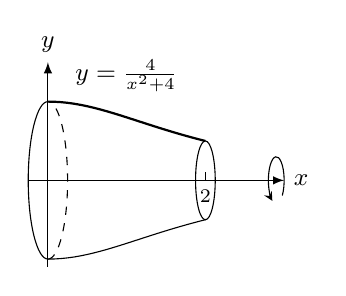
\begin{tikzpicture}[font=\small,declare function={f(\x)=4/(\x^2+4);}]
\pgfmathsetmacro{\ra}{f(0)}
\pgfmathsetmacro{\rb}{f(2)}
\draw[-latex](-0.25,0)--(3,0)node[right]{$x$};
\draw[-latex](0,-1.1)--(0,1.5)node[above]{$y$};
\draw[-stealth] ([shift={(-40:1/3*0.3 cm and 0.3 cm)}]2.9,0) arc (-40:240:1/3*0.3 cm and 0.3 cm);
\draw[thick,domain=0:2] plot({\x},{f(\x)});
\draw[domain=0:2] plot({\x},{-f(\x)});
\draw([shift={(90:1/4*\ra cm and \ra cm)}]0,0) arc (90:270:1/4*\ra cm and \ra cm);
\draw[dashed]([shift={(-90:1/4*\ra cm and \ra cm)}]0,0) arc (-90:90:1/4*\ra cm and \ra cm);
\draw(2,0) circle (1/4*\rb cm and \rb cm);
\draw(1,1)node[above]{$y=\frac{4}{x^2+4}$};
\draw(2,0)node[below,font=\scriptsize]{$2$}--++(0,0.1);
\end{tikzpicture}
\caption{}
\end{subfigure}\hfill
\begin{subfigure}{0.30\textwidth}
\centering
\begin{tikzpicture}
\pgfmathsetmacro{\r}{2}
\pgfmathsetmacro{\ang}{30}
\draw(0,0)--++(\ang:\r)coordinate(ka)node[pos=0.7,left,yshift=1ex]{$\sqrt{x^2+4}$}--($(0,0)!(ka)!(2,0)$)node[pos=0.5,right]{$x$}--(0,0)node[pos=0.5,below]{$2$};
\draw([shift={(0:0.5)}]0,0) arc (0:\ang:0.5);
\draw(1/2*\ang:0.7)node[]{$\theta$};
\draw(\r/2,{\r*sin(\ang)})node[above,yshift=1ex]{$\tan\theta=\frac{x}{2}$};
\end{tikzpicture}
\caption{}
\end{subfigure}
\caption{خطہ، جسم طواف اور حوالہ مثلث برائے مثال \حوالہ{مثال_طریقہ_جسم_طواف_حوالہ_مثلث}}
\label{شکل_مثال_طریقہ_جسم_طواف_حوالہ_مثلث}
\end{figure}

%==========================

\موٹا{بدل $z=\tan(\tfrac{x}{2})$}\\
\عددی{\sin x} اور \عددی{\cos x} کے ناطق تفاعل کے تکمل کو درج ذیل بدل
\begin{align}\label{مساوات_طریقہ_ٹینجنٹ_بدل}
z=\tan\frac{x}{2}
\end{align}
متغیر \عددی{z} کے ناطق تفاعل کے تکمل میں بدلتا ہے جس کو جزوی کسری مجموعہ لکھ کر حل کیا جا سکتا ہے۔ یوں مساوات \حوالہ{مساوات_طریقہ_ٹینجنٹ_بدل} کا بدل انتہائی طاقتور ثابت ہوتا ہے اگرچہ اس کا استعمال زیادہ آسان نہیں ہے اور صرف وہاں استعمال کیا جاتا ہے جب باقی تراکیب مددگار ثابت نہ ہوں۔

\begin{figure}
\centering
\begin{tikzpicture}[font=\small]
\pgfmathsetmacro{\r}{1.25}
\pgfmathsetmacro{\ang}{60}
\draw[-latex](-\r-0.5,0)--(\r+0.5,0);
\draw(0,0) circle (\r);
\draw(0,0)--++(\ang:\r)node[above right]{$N(\cos x,\sin x)$}node[pos=0.5,left]{$1$}coordinate(kt){}--($(0,0)!(kt)!(\r,0)$)node[pos=0.6,above,sloped]{$\sin x$}--(0,0)node[pos=0.5,below]{$\cos x$};
\draw(kt)--(-\r,0)node[below left] {$A$};
\draw([shift={(0:0.3)}]0,0) arc (0:\ang:0.3);
\draw([shift={(0:0.6)}]-\r,0) arc (0:1/2*\ang:0.6);
\draw(1/2*\ang:0.45)node[]{$x$};
\draw(-\r,0)++(1/4*\ang:0.8)node[]{$\tfrac{x}{2}$};
\end{tikzpicture}
\caption{ہم شکل سے $\tan\tfrac{x}{2}=\tfrac{\sin x}{1+\cos x}$ پڑھ سکتے ہیں۔}
\label{شکل_طریقہ_سوال_بدل_ٹینجنٹ}
\end{figure}
\عددی{\sin x} اور \عددی{\cos x} کے ناطق تفاعل کو \عددی{\tan\tfrac{x}{2}} کی صورت میں لکھنا شکل \حوالہ{شکل_طریقہ_سوال_بدل_ٹینجنٹ} میں دکھایا گیا ہے۔ درج ذیل کی مدد سے ہم بدل کے اثر کو دیکھتے ہیں۔
\begin{gather}
\begin{aligned}\label{مساوات_طریقہ_ٹینجنٹ_بدل_الف}
\cos x&=2\cos^2\frac{x}{2}-1=\frac{2}{\sec^2\frac{x}{2}}-1\\
&=\frac{2}{1+\tan^2\frac{x}{2}}-1=\frac{2}{1+z^2}-1\\
\cos x&=\frac{1-z^2}{1+z^2}
\end{aligned}
\end{gather}
اور
\begin{gather}
\begin{aligned}\label{مساوات_طریقہ_ٹینجنٹ_بدل_ب}
\sin x&=2\sin\frac{x}{2}\cos\frac{x}{2}=2\frac{\sin\frac{x}{2}}{\cos\frac{x}{2}}\cdot\cos^2\frac{x}{2}\\
&=2\tan\frac{x}{2}\cdot\frac{1}{\sec^2\frac{x}{2}}=\frac{2\tan\frac{x}{2}}{1+\tan^2\frac{x}{2}}\\
\sin x&=\frac{2z}{1+z^2}
\end{aligned}
\end{gather}
اور
\begin{align}\label{مساوات_طریقہ_ٹینجنٹ_بدل_پ}
\dif x=\frac{2\dif z}{1+z^2}
\end{align}

\ابتدا{مثال}
\begin{align*}
\text{\RL{(الف)}}\quad \int\frac{\dif x}{1+\cos x}&=\int\frac{1+z^2}{2}\frac{2\dif z}{1+z^2}\\
&=\int \dif z=z+C\\
&=\tan\frac{x}{2}+C\\
\text{\RL{(ب)}}\quad \int\frac{\dif x}{2+\sin x}&=\int\frac{1+z^2}{2+2z+2z^2}\frac{2\dif z}{1+z^2}\\
&=\int\frac{\dif z}{z^2+z+1}=\int\frac{\dif z}{(z+1/2)^2+3/4}\\
&=\int\frac{\dif u}{u^2+a^2}\\
&=\frac{1}{a}\tan^{-1}\frac{u}{a}+C\\
&=\frac{2}{\sqrt{3}}\tan^{-1}\frac{2z+1}{\sqrt{3}}+C\\
&=\frac{2}{\sqrt{3}}\tan^{-1}\frac{1+2\tan(x/2)}{\sqrt{3}}+C
\end{align*}
\انتہا{مثال}
%======================
\حصہء{سوالات}
\موٹا{بنیادی تکونیاتی بدل}\\
سوال \حوالہ{سوال_طریقہ_بنیادی_تکونیاتی_تکمل_الف} تا سوال \حوالہ{سوال_طریقہ_بنیادی_تکونیاتی_تکمل_ب} میں تکمل حل کریں۔

\ابتدا{سوال}\شناخت{سوال_طریقہ_بنیادی_تکونیاتی_تکمل_الف}
$\int\frac{\dif y}{\sqrt{9+y^2}}$\\
جواب:\quad
$\ln\abs{\sqrt{9+y^2}+y}+C$
\انتہا{سوال}
%======================
\ابتدا{سوال}
$\int\frac{3\dif y}{\sqrt{1+9y^2}}$
\انتہا{سوال}
%======================
\ابتدا{سوال}
$\int_{-2}^2\frac{\dif x}{4+x^2}$\\
جواب:\quad
$\tfrac{\pi}{4}$
\انتہا{سوال}
%======================
\ابتدا{سوال}
$\int_0^2\frac{\dif x}{8+2x^2}$
\انتہا{سوال}
%======================
\ابتدا{سوال}
$\int_0^{3/2}\frac{\dif x}{\sqrt{9-x^2}}$\\
جواب:\quad
$\tfrac{\pi}{6}$
\انتہا{سوال}
%======================
\ابتدا{سوال}
$\int_0^{1/2\sqrt{2}}\frac{2\dif x}{\sqrt{1-4x^2}}$
\انتہا{سوال}
%======================
\ابتدا{سوال}
$\int\sqrt{25-t^2}\dif t$\\
جواب:\quad
$\tfrac{25}{2}\sin^{-1}\tfrac{t}{5}+\tfrac{t\sqrt{25-t^2}}{2}+C$
\انتہا{سوال}
%======================
\ابتدا{سوال}
$\int\sqrt{1-9t^2}\dif t$
\انتہا{سوال}
%======================
\ابتدا{سوال}
$\int\frac{\dif x}{\sqrt{4x^2-49}},\quad x>\frac{7}{2}$\\
جواب:\quad
$\tfrac{1}{2}\ln\abs{\tfrac{2x}{7}+\tfrac{\sqrt{4x^2-49}}{7}}+C$
\انتہا{سوال}
%======================
\ابتدا{سوال}
$\int\frac{5\dif x}{\sqrt{25x^2-9}},\quad x>\frac{3}{5}$
\انتہا{سوال}
%======================
\ابتدا{سوال}
$\int\frac{\sqrt{y^2-49}}{y}\dif y,\quad y>7$\\
جواب:\quad
$7[\tfrac{\sqrt{y^2-49}}{7}-\sec^{-1}\tfrac{y}{7}]+C$
\انتہا{سوال}
%======================
\ابتدا{سوال}
$\int\frac{\sqrt{y^2-25}}{y^3}\dif y,\quad y>5$
\انتہا{سوال}
%======================
\ابتدا{سوال}
$\int\frac{\dif x}{x^2\sqrt{x^2-1}},\quad x>1$\\
جواب:\quad
$\tfrac{\sqrt{x^2-1}}{x}+C$ 
\انتہا{سوال}
%======================
\ابتدا{سوال}
$\int\frac{2\dif x}{x^3\sqrt{x^2-1}},\quad x>1$
\انتہا{سوال}
%======================
\ابتدا{سوال}
$\int\frac{x^3\dif x}{\sqrt{x^2+4}}$\\
جواب:\quad
$\tfrac{1}{3}(x^2+4)^{3/2}-4\sqrt{x^2+4}+C$
\انتہا{سوال}
%======================
\ابتدا{سوال}
$\int\frac{\dif x}{x^2\sqrt{x^2+1}}$
\انتہا{سوال}
%======================
\ابتدا{سوال}
$\int\frac{8\dif w}{w^2\sqrt{4-w^2}}$\\
جواب:\quad
$\tfrac{-2\sqrt{4-w^2}}{w}+C$ 
\انتہا{سوال}
%======================
\ابتدا{سوال}
$\int\frac{\sqrt{9-w^2}}{w^2}\dif w$
\انتہا{سوال}
%======================
\ابتدا{سوال}
$\int_0^{\sqrt{3}/2}\frac{4x^2\dif x}{(1-x^2)^{3/2}}$\\
جواب:\quad
$4\sqrt{3}-\tfrac{4\pi}{3}$
\انتہا{سوال}
%======================
\ابتدا{سوال}
$\int_0^1\frac{\dif x}{(4-x^2)^{3/2}}$
\انتہا{سوال}
%======================
\ابتدا{سوال}
$\int\frac{\dif x}{(x^2-1)^{3/2}},\quad x>1$\\
جواب:\quad
$\tfrac{-x}{\sqrt{x^2-1}}+C$
\انتہا{سوال}
%======================
\ابتدا{سوال}
$\int\frac{x^2\dif x}{(x^2-1)^{5/2}},\quad x>1$
\انتہا{سوال}
%======================
\ابتدا{سوال}
$\int\frac{(1-x^2)^{3/2}}{x^6}\dif x$\\
جواب:\quad
$-\tfrac{1}{5}\big(\tfrac{\sqrt{1-x^2}}{x}\big)^5+C$
\انتہا{سوال}
%======================
\ابتدا{سوال}
$\int\frac{(1-x^2)^{1/2}}{x^4}\dif x$
\انتہا{سوال}
%======================
\ابتدا{سوال}
$\int\frac{8\dif x}{(4x^2+1)^2}$\\
جواب:\quad
$2\tan^{-1}2x+\tfrac{4x}{4x^2+1}+C$ 
\انتہا{سوال}
%======================
\ابتدا{سوال}
$\int\frac{6\dif t}{(9t^2+1)^2}$
\انتہا{سوال}
%======================
\ابتدا{سوال}
$\int\frac{v^2\dif v}{(1-v^2)^{5/2}}$\\
جواب:\quad
$\tfrac{1}{3}\big(\tfrac{v}{\sqrt{1-v^2}}\big)^3+C$
\انتہا{سوال}
%======================
\ابتدا{سوال}\شناخت{سوال_طریقہ_بنیادی_تکونیاتی_تکمل_ب}
$\int\frac{(1-r^2)^{5/2}}{r^8}\dif r$
\انتہا{سوال}
%======================
\موٹا{موزوں بدل کے بعد تکونیاتی بدل استعمال کرتے ہوئے سوال \حوالہ{سوال_بدل_تکونیاتی_حل_تکمل_الف} تا سوال \حوالہ{سوال_بدل_تکونیاتی_حل_تکمل_ب}  میں تکمل حل کریں۔}

\ابتدا{سوال}\شناخت{سوال_بدل_تکونیاتی_حل_تکمل_الف}
 $\int_0^{\ln 4}\frac{e^t\dif t}{\sqrt{e^{2t}+9}}$\\
جواب:\quad
$\ln 9-\ln(1+\sqrt{10})$
\انتہا{سوال}
%=======================
\ابتدا{سوال}
 $\int_{\ln(3/4)}^{\ln(4/3)}\frac{e^t\dif t}{(1+e^{2t})^{3/2}}$
\انتہا{سوال}
%=======================
\ابتدا{سوال}
 $\int_{1/12}^{1/4}\frac{2\dif t}{\sqrt{t}+4t\sqrt{t}}$\\
جواب:\quad
$\tfrac{\pi}{6}$
\انتہا{سوال}
%=======================
\ابتدا{سوال}
 $\int_1^e\frac{\dif y}{y\sqrt{1+(\ln y)^2}}$
\انتہا{سوال}
%=======================
\ابتدا{سوال}
 $\int\frac{\dif x}{x\sqrt{x^2-1}}$\\
جواب:\quad
$\sec^{-1}\abs{x}+C$
\انتہا{سوال}
%=======================
\ابتدا{سوال}
 $\int\frac{\dif x}{1+x^2}$
\انتہا{سوال}
%=======================
\ابتدا{سوال}
 $\int\frac{x\dif x}{\sqrt{x^2-1}}$\\
جواب:\quad
$\sqrt{x^2-1}+C$
\انتہا{سوال}
%=======================
\ابتدا{سوال}\شناخت{سوال_بدل_تکونیاتی_حل_تکمل_ب}
 $\int\frac{\dif x}{\sqrt{1-x^2}}$
\انتہا{سوال}
%=======================
\موٹا{ابتدائی قیمت مسائل}\\
سوال \حوالہ{سوال_طریقہ_ابتدائی_قیمت_بدل_الف} تا سوال \حوالہ{سوال_طریقہ_ابتدائی_قیمت_بدل_ب} کے ابتدائی قیمت مسائل حل کرتے ہوئے \عددی{y} حاصل کریں۔

\ابتدا{سوال}\شناخت{سوال_طریقہ_ابتدائی_قیمت_بدل_الف}
$x\frac{\dif y}{\dif x}=\sqrt{x^2-4},\quad x\ge 2,\quad y(2)=0$\\
جواب:\quad
$y=2[\tfrac{\sqrt{x^2-4}}{2}-\sec^{-1}\tfrac{x}{2}]$
\انتہا{سوال}
%=====================
\ابتدا{سوال}
$\sqrt{x^2-9}\frac{\dif y}{\dif x}=1,\quad x>3,\quad y(5)=\ln 3$
\انتہا{سوال}
%=====================
\ابتدا{سوال}
$(x^2+4)\frac{\dif y}{\dif x}=3,\quad y(2)=0$\\
جواب:\quad
$y=\tfrac{3}{2}\tan^{-1}\tfrac{x}{2}-\tfrac{3\pi}{8}$
\انتہا{سوال}
%=====================
\ابتدا{سوال}\شناخت{سوال_طریقہ_ابتدائی_قیمت_بدل_ب}
$(x^2+1)^2\frac{\dif y}{\dif x}=\sqrt{x^2+1},\quad y(0)=1$
\انتہا{سوال}
%=====================
\موٹا{استعمال}

\ابتدا{سوال}
ربع اول میں محددی محور اور منحنی \عددی{y=\tfrac{\sqrt{9-x^2}}{3}} کے بیچ رقبہ تلاش کریں۔\\
جواب:\quad
$\tfrac{3\pi}{4}$
\انتہا{سوال}
%========================
\ابتدا{سوال}
ربع اول میں محددی محور، لکیر \عددی{x=1} اور منحنی \عددی{y=\tfrac{2}{1+x^2}} کے بیچ خطہ کو محور \عددی{x} کے گرد گھما کر جسم طواف پیدا کیا جاتا ہے۔ اس جسم کا حجم تلاش کریں۔
\انتہا{سوال}
%========================
\موٹا{بدل $z=\tan(x/2)$}\\
سوال \حوالہ{سوال_طریقہ_ٹینجنٹ_بدل_الف} تا سوال \حوالہ{سوال_طریقہ_ٹینجنٹ_بدل_ب} کو  مساوات \حوالہ{مساوات_طریقہ_ٹینجنٹ_بدل_الف} تا مساوات \حوالہ{مساوات_طریقہ_ٹینجنٹ_بدل_پ} کی مدد سے حل کریں۔ 

\ابتدا{سوال}\شناخت{سوال_طریقہ_ٹینجنٹ_بدل_الف}
$\int\frac{\dif x}{1-\sin x}$\\
جواب:\quad
$\tfrac{2}{1-\tan\tfrac{x}{2}}+C$
\انتہا{سوال}
%=====================
\ابتدا{سوال}
$\int\frac{\dif x}{1+\sin x+\cos x}$
\انتہا{سوال}
%=====================
\ابتدا{سوال}
$\int_0^{\pi/2}\frac{\dif x}{1+\sin x}$\\
جواب:\quad
$1$
\انتہا{سوال}
%=====================
\ابتدا{سوال}
$\int_{\pi/3}^{\pi/2}\frac{\dif x}{1-\cos x}$
\انتہا{سوال}
%=====================
\ابتدا{سوال}
$\int_0^{\pi/2}\frac{\dif\theta}{2+\cos\theta}$\\
جواب:\quad
$\tfrac{\sqrt{3}\pi}{9}$
\انتہا{سوال}
%=====================
\ابتدا{سوال}
$\int_{\pi/2}^{2\pi/3}\frac{\cos\theta\dif\theta}{\sin\theta\cos\theta+\sin\theta}$
\انتہا{سوال}
%=====================
\ابتدا{سوال}
$\int\frac{\dif t}{\sin t-\cos t}$\\
جواب:\quad
$\tfrac{1}{\sqrt{2}}\ln\abs{\tfrac{\tan(t/2)+1-\sqrt{2}}{\tan(t/2)+1+\sqrt{2}}}+C$
\انتہا{سوال}
%=====================
\ابتدا{سوال}\شناخت{سوال_طریقہ_ٹینجنٹ_بدل_ب}
$\int\frac{\cos t\dif t}{1-\cos t}$
\انتہا{سوال}
%=====================
درج ذیل دو سوالات میں \عددی{z=\tan(\theta/2)} پر کر کے حل کریں۔\\
\ابتدا{سوال}
$\int\sec\theta\dif\theta$\\
جواب:\quad
$\ln\abs{\tfrac{1+\tan(\theta/2)}{1-\tan(\theta/2)}}+C$
\انتہا{سوال}
%=====================
\ابتدا{سوال}
$\int\csc\theta\dif\theta$
\انتہا{سوال}
%=====================

\حصہ{جدول تکمل اور کمپیوٹر}\شناخت{حصہ_تراکیب_تکمل_جدول_تکمل_اور_کمپیوٹر}
جیسا آپ جانتے ہیں تکمل کے بنیادی طریقے بدل اور تکمل بالحصص ہیں۔ان طریقوں سے  ہم انجانے تکمل کو جانے پہچانے تکمل میں بدلتے ہیں جس کو ہم حل کرنا جانتے ہیں یا جس کو جدول سے دیکھا جا سکتا ہے۔ ان جدول میں تکمل کہاں سے آتے ہیں؟ جدول میں تکمل بھی بدل یا تکمل بالحصص سے حاصل کیے گئے ہوتے ہیں۔ ہم ان تمام کو خود حاصل کر سکتے ہیں لیکن جدول ہمیں بار بار ایک ہی طرز کے تکمل حاصل کرنے سے چھٹکارا دیتا ہے۔ جب کوئی تکمل جدول میں پایا جاتا ہو یا الجبرا، تکونیات، بدل اور احصاء کی استعمال سے اس کو جدول میں درج کسی تکمل کی صورت میں لانا ممکن ہو، تب ہم تکمل کا حل جدول سے پڑھ سکتے ہیں۔ اس حصہ کی مثالوں اور سوالات میں  کتاب کی آخر میں صفحہ \حوالہصفحہ{ضمیمہ_جدول_تکملات} پر تکملات کی جدول میں درج کلیات کو اخذ کرنا اور ان کا استعمال سکھایا جائے گا۔ یہاں استعمال پر زور دیا جائے گا۔ کتاب کے آخر میں کلیات کو مستقل \عددی{a,b,c,m,n}  وغیرہ کی صورت میں لکھا گیا ہے۔ یہ مستقل عموماً حقیقی اعداد ہوں گے جو غیر عدد صحیح ہو سکتے ہیں۔ جہاں ان مستقل پر شرائط مسلط ہو، وہاں اس کا ذکر کیا گیا ہے۔ مثال کے طور پر کلیہ \حوالہ{مساوات_جدول_تکمل_پانچ} میں \عددی{n\ne -1} ہونا ضروری ہے جبکہ کلیہ  \حوالہ{مساوات_جدول_تکمل_گیارہ} میں \عددی{n\ne -2} ہونا ضروری ہے۔ 

ان کلیات میں  مستقل وہ قیمت اختیار نہیں کر سکتے ہیں جن کی بنا صفر سے تقسیم کرنا پڑے یا منفی اعداد کا جفت جذر لینا پڑے۔ مثال کے طور پر کلیہ \حوالہ{مساوات_جدول_تکمل_آٹھ} میں \عددی{a\ne 0} ہو گا جبکہ کلیہ \حوالہ{مساوات_جدول_تکمل_تیرہ}-الف صرف اس صورت قابل استعمال ہو گا جب \عددی{b} منفی ہو۔ 

بہت سارے غیر قطعی تکمل کو کمپیوٹر کی مدد سے بھی حل کیا جا سکتا ہے جہاں تکمل کو کسی خاص صورت میں لکھنے کی ضرورت پیش نہیں آتی ہے۔ کمپیوٹر الجبرا پر اس حصہ کے آخر میں غور کیا جائے گا۔

\جزوحصہء{جدول کی مدد سے تکمل}
\ابتدا{مثال}
تکمل \عددی{\int x(2x+5)^{-1}\dif x} حل کریں۔

حل:\quad
ہم کلیہ \حوالہ{مساوات_جدول_تکمل_آٹھ} استعمال کرتے ہیں (نا کہ کلیہ \حوالہ{مساوات_جدول_تکمل_سات} جہاں \عددی{n\ne -1} ہونا ضروری ہے۔)
\begin{align*}
\int x(ax+b)^{-1}\dif x=\frac{x}{a}-\frac{b}{a^2}\ln\abs{ax+b}+C
\end{align*}
یوں \عددی{a=2} اور \عددی{b=5} کی صورت میں درج ذیل ہو گا۔
\begin{align*}
\int x(2x+5)^{-1}\dif x=\frac{x}{2}-\frac{5}{4}\ln\abs{2x+5}+C
\end{align*}
\انتہا{مثال}
%===============
\ابتدا{مثال}
تکمل \عددی{\int\frac{\dif x}{x\sqrt{2x+4}}} حل کریں۔

حل:\quad
ہم کلیہ \حوالہ{مساوات_جدول_تکمل_تیرہ}-ب استعمال کرتے ہیں۔
\begin{align*}
\int\frac{\dif x}{x\sqrt{ax+b}}&=\frac{1}{\sqrt{b}}\ln\abs{\frac{\sqrt{ax+b}-\sqrt{b}}{\sqrt{ax+b}+\sqrt{b}}}+C&&\text{\RL{اگر $b>0$ ہو}}
\end{align*}
یوں \عددی{a=2} اور \عددی{b=4} کی صورت میں درج ذیل ہو گا۔
\begin{align*}
\int\frac{\dif x}{x\sqrt{2x+4}}&=\frac{1}{\sqrt{4}}\ln\abs{\frac{\sqrt{2x+4}-\sqrt{4}}{\sqrt{2x+4}+\sqrt{4}}}+C\\
&=\frac{1}{2}\ln\abs{\frac{\sqrt{2x+4}-2}{\sqrt{2x+4}+2}}+C
\end{align*}
کلیہ \حوالہ{مساوات_جدول_تکمل_تیرہ}-الف یہاں قابل استعمال نہیں ہو گا چونکہ اس میں \عددی{b<0} ضروری ہے، البتہ اگلی مثال میں یہ کارآمد ہو گا۔
\انتہا{مثال}
%====================
\ابتدا{مثال}\شناخت{مثال_طریقہ_تکمل_استعمال_کلیات_تیسرا}
تکمل \عددی{\int\frac{\dif x}{x\sqrt{2x-4}}} حل کریں۔

حل:\quad
ہم کلیہ \حوالہ{مساوات_جدول_تکمل_تیرہ}-الف استعمال کرتے ہیں۔
\begin{align*}
\int\frac{\dif x}{x\sqrt{ax-b}}=\frac{2}{\sqrt{b}}\tan^{-1}\sqrt{\frac{ax-b}{b}}+C
\end{align*}
یوں \عددی{a=2} اور \عددی{b=4} لیتے ہوئے درج ذیل ہو گا۔
\begin{align*}
\int \frac{\dif x}{x\sqrt{2x-4}}=\frac{2}{\sqrt{4}}\tan^{-1}\sqrt{\frac{2x-4}{4}}+C=\tan^{-1}\sqrt{\frac{x-2}{2}}+C
\end{align*}
\انتہا{مثال}
%=============
\ابتدا{مثال}
تکمل \عددی{\int \frac{\dif x}{x^2\sqrt{2x-4}}} حل کریں۔

حل:\quad
ہم کلیہ \حوالہ{مساوات_جدول_تکمل_پندرہ} سے شروع کرتے ہیں۔
\begin{align*}
\int\frac{\dif x}{x^2\sqrt{ax+b}}=-\frac{\sqrt{ax+b}}{bx}-\frac{a}{2b}\int\frac{\dif x}{x\sqrt{ax+b}}+C
\end{align*}
یوں \عددی{a=2} اور \عددی{b=-4} لیتے ہوئے
\begin{align*}
\int\frac{\dif x}{x^2\sqrt{2x-4}}=-\frac{\sqrt{2x-4}}{-4x}+\frac{2}{2\cdot 4}\int\frac{\dif x}{x\sqrt{2x-4}}+C
\end{align*}
ملتا ہے۔ اب ہم کلیہ \حوالہ{مساوات_جدول_تکمل_تیرہ}-الف استعمال کرتے ہوئے دائیں ہاتھ تکمل حل کرتے ہیں (مثال \حوالہ{مثال_طریقہ_تکمل_استعمال_کلیات_تیسرا} سے رجوع کریں):
\begin{align*}
\int\frac{\dif x}{x^2\sqrt{2x-4}}=\frac{\sqrt{2x-4}}{4x}+\frac{1}{4}\tan^{-1}\sqrt{\frac{x-2}{2}}+C
\end{align*}
\انتہا{مثال}
%=================
\ابتدا{مثال}
تکمل \عددی{\int x\sin^{-1}x\dif x} حل کریں۔

حل:\quad
ہم کلیہ \حوالہ{مساوات_جدول_تکمل_ننانوے} استعمال کرتے ہیں۔
\begin{align*}
\int x^n\sin^{-1}ax\dif x=\frac{x^{n+1}}{n+1}\sin^{-1}ax-\frac{a}{n+1}\int\frac{x^{n+1}\dif x}{\sqrt{1-a^2x^2}},\quad n\ne -1
\end{align*}
یوں \عددی{n=1} اور \عددی{a=1} لے کر
\begin{align*}
\int x\sin^{-1}x\dif x=\frac{x^2}{2}\sin^{-1}x-\frac{1}{2}\int\frac{x^2\dif x}{\sqrt{1-x^2}}
\end{align*}
ہو گا۔ دائیں ہاتھ تکمل جدول میں کلیہ \حوالہ{مساوات_جدول_تکمل_تینتیس} ہے:
\begin{align*}
\int \frac{x^2}{\sqrt{a^2-x^2}}\dif x=\frac{a^2}{2}\sin^{-1}\frac{x}{a}-\frac{1}{2}x\sqrt{a^2-x^2}+C
\end{align*}
اب \عددی{a=1} کے لئے درج ذیل ہو گا۔
\begin{align*}
\int \frac{x^2}{\sqrt{1-x^2}}\dif x=\frac{1}{2}\sin^{-1}x-\frac{1}{2}x\sqrt{1-x^2}+C
\end{align*}
یوں مجموعی حل درج ذیل ہو گا۔
\begin{align*}
\int x\sin^{-1}x\dif x&=\frac{x^2}{2}\sin^{-1}x-\frac{1}{2}\big(\frac{1}{2}\sin^{-1}x-\frac{1}{2}x\sqrt{1-x^2}\big)+C'\\
&=\big(\frac{x^2}{2}-\frac{1}{4}\big)\sin^{-1}x+\frac{1}{4}x\sqrt{1-x^2}+C'
\end{align*}
\انتہا{مثال}
%=======================

\جزوحصہء{کلیات تخفیف}
دہراتے ہوئے تکمل بالحصص میں درج ذیل صورت کے کلیات مددگار ثابت ہوتے ہیں جنہیں \اصطلاح{کلیات تخفیف}\فرہنگ{کلیات!تخفیف}\فرہنگ{تخفیف!کلیات}\حاشیہب{reduction formulae}\فرہنگ{reduction formulae} کہتے ہیں۔
\begin{align}
\int \tan^n x\dif x&=\frac{1}{n-1}\tan^{n-1}x-\int \tan^{n-2}x\dif x\label{مساوات_طریقہ_کلیات_تخفیف_الف}\\
\int(\ln x)^n\dif x&=x(\ln x)^n-n\int(\ln x)^{n-1}\label{مساوات_طریقہ_کلیات_تخفیف_ب}\\
\int\sin^nx\cos^mx\dif x&=-\frac{\sin^{n-1}x\cos^{m+1}x}{m+n}\dif x\nonumber\\
&\phantom{=}+\frac{n-1}{m+n}\int\sin^{n-2}x\cos^mx\dif x,\quad (n\ne -m)\label{مساوات_طریقہ_کلیات_تخفیف_پ}
\end{align}
کلیات تخفیف کسی تفاعل کے طاقت کے تکمل کو اسی طرز کے تکمل جس میں تفاعل کی طاقت کم ہو سے تبدیل کرتا ہے۔ طاقت کی تخفیف کی بنا انہیں کلیات تخفیف کہتے ہیں۔ کلیات تخفیف بار بار استعمال کرتے ہوئے آخر کار تکمل میں تفاعل کی طاقت اتنی کم ہو جاتی ہے کہ تکمل با آسانی حل ہوتا ہے۔

\ابتدا{مثال}
تکمل \عددی{\int \tan^5x\dif x} حل کریں۔

حل:\quad
ہم \عددی{n=5} لیتے ہوئے مساوات \حوالہ{مساوات_طریقہ_کلیات_تخفیف_الف} استعمال کرتے ہیں۔
\begin{align*}
\int\tan^5x\dif x=\frac{1}{4}\tan^4x-\int\tan^3x\dif x
\end{align*}
ہم \عددی{n=3} لیتے ہوئے  مساوات \حوالہ{مساوات_طریقہ_کلیات_تخفیف_الف} دوبارہ استعمال کرتے ہیں۔
\begin{align*}
\int\tan^3x\dif x=\frac{1}{2}\tan^2x-\int \tan x\dif x=\frac{1}{2}\tan^2x+\ln\abs{\cos x}+C
\end{align*}
یوں مکمل نتیجہ درج ذیل ہو گا۔
\begin{align*}
\int^5x \dif x=\frac{1}{4}\tan^4x-\frac{1}{2}\tan^2x-\ln\abs{\cos x}+C
\end{align*}
\انتہا{مثال}
%==========
کلیات تخفیف کو تکمل بالحصص سے حاصل کیا جاتا ہے۔

\ابتدا{مثال}\ترچھا{کلیات تخفیف کا حصول}\\
کسی بھی مثبت عدد صحیح \عددی{n} کے لئے درج ذیل کی تصدیق کریں۔
\begin{align*}
\int (\ln x)^n\dif x=x(\ln x)^n-n\int (\ln x)^{n-1}\dif x
\end{align*}
حل:\quad
ہم تکمل بالحصص کے کلیہ
\begin{align*}
\int u\dif v=uv-\int v\dif u
\end{align*}
میں
\begin{align*}
u=(\ln x)^n,\quad \dif u=n(\ln x)^{n-1}\frac{\dif x}{x},\quad \dif v=\dif x,\quad v=x
\end{align*}
لے کر درج ذیل حاصل کرتے ہیں۔
\begin{align*}
\int (\ln x)^n\dif x=x(\ln x)^n-n\int (\ln x)^{n-1}\dif x
\end{align*}
\انتہا{مثال}
%===================
بعض اوقات دو کلیات تخفیف کا استعمال ضروری ہو گا۔

\ابتدا{مثال}
تکمل \عددی{\int\sin^2x\cos^3x\dif x} حل کریں۔

حل الف:\quad
ہم مساوات \حوالہ{مساوات_طریقہ_کلیات_تخفیف_پ} میں \عددی{n=2} اور \عددی{m=3} لے کر درج ذیل حاصل کرتے ہیں۔
\begin{align*}
\int \sin^2x\cos^3x\dif x&=-\frac{\sin x\cos^4x}{2+3}+\frac{1}{2+3}\int\sin^0x\cos^3x\dif x\\
&=-\frac{\sin x\cos^4x}{5}+\frac{1}{5}\int\cos^3x\dif x
\end{align*}
ہم باقی تکمل کو کلیہ \حوالہ{مساوات_جدول_تکمل_اکسٹھ} سے حل کر سکتے ہیں۔
\begin{align*}
\int\cos^nax\dif x=\frac{\cos^{n-1}ax\sin ax}{na}+\frac{n-1}{n}\int\cos^{n-2}ax\dif x
\end{align*}
یوں \عددی{n=3} اور \عددی{a=1} لیتے ہوئے
 \begin{align*}
\int\cos^3x\dif x&=\frac{\cos^2x\sin x}{3}+\frac{2}{3}\int\cos x\dif x\\
&=\frac{\cos^2x\sin x}{3}+\frac{2}{3}\sin x+C
\end{align*}
حاصل ہو گا۔مجموعی نتیجہ درج ذیل ہو گا۔
\begin{align*}
\int\sin^2x\cos^3x\dif x &=-\frac{\sin x\cos^4x}{5}+\frac{1}{5}\big(\frac{\cos^2x\sin x}{3}+\frac{2}{3}\sin x+C\big)\\
&=-\frac{\sin x\cos^4 x}{5}+\frac{\cos^2x\sin x}{15}+\frac{2}{15}\sin x+C'
\end{align*}

حل ب:\quad
مساوات \حوالہ{مساوات_طریقہ_کلیات_تخفیف_پ} جدول میں کلیہ \حوالہ{مساوات_جدول_تکمل_اٹسٹھ} ہے ، مگر ہم کلیات تکمل کے جدول کا کلیہ \حوالہ{مساوات_جدول_تکمل_انتر} بھی استعمال کر سکتے ہیں جس میں \عددی{a=1} لیتے ہوئے
\begin{align*}
\int \sin^nx\cos^mx\dif x=\frac{\sin^{n+1}x\cos^{m-1}x}{m+n}+\frac{m-1}{m+n}\int \sin^nx\cos^{m-2}x\dif x
\end{align*}
لکھا جائے گا۔ اب \عددی{n=2} اور \عددی{m=3} لیتے ہوئے درج ذیل ملتا ہے۔
\begin{align*}
\int\sin^2x\cos^3x\dif x&=\frac{\sin^3x\cos^2x}{5}+\frac{2}{5}\int\sin^2x\cos x\dif x\\
&=\frac{\sin^3x\cos^2x}{5}+\frac{2}{5}\big(\frac{\sin^3x}{3}\big)+C\\
&=\frac{\sin^3x\cos^2x}{5}+\frac{2}{15}\sin^3x+C
\end{align*} 
آپ نے دیکھا کہ کلیہ  \حوالہ{مساوات_جدول_تکمل_انتر} زیادہ جلدی نتیجہ فراہم کرتا ہے۔ عموماً قبل از وقت یہ جاننا ممکن نہیں ہوتا ہے کہ کونسا کلیہ زیادہ جلدی نتیجہ دیگا گا۔ اس پر وقت ضائع نہ کریں۔ جو بھی کلیہ قابل استعمال نظر آئے، اس کو فوراً استعمال کریں۔

آپ نے یہ بھی دیکھا ہو گا کہ کلیہ \حوالہ{مساوات_جدول_تکمل_اٹسٹھ} اور کلیہ \حوالہ{مساوات_جدول_تکمل_انتر} کے نتائج مختلف نظر آتے ہیں۔ تکونیاتی تکمل میں عموماً ایسا ہی ہو گا۔ آپ فکر نہ کریں چونکہ ایسے نتائج درحقیقت بالکل ایک دوسرے جیسے ہوں گے۔
\انتہا{مثال}
%=============== 

\جزوحصہء{غیر بنیادی تکمل}
وہ الٹ تفرق جنہیں بنیادی تفاعل (وہ تفاعل جن پر اب تک غور کیا گیا) کی صورت میں لکھنا ممکن نہ ہو \اصطلاح{غیر بنیادی}\فرہنگ{تکمل!غیر بنیادی}\فرہنگ{غیر بنیادی تکمل}\حاشیہب{nonelementary}\فرہنگ{nonelementary} تکمل کہلاتے ہیں۔ غیر بنیادی تکمل کا حل لامتناہی سلسلہ  یا اعدادی تراکیب سے حاصل ہو گا۔ اعدادی تراکیب سے حل ہونے والے تکمل میں تفاعل خلل
\begin{align*}
\erf(x)=\frac{2}{\pi}\int_0^x e^{-t^2}\dif t
\end{align*}
اور درج ذیل قسم کے تکمل شامل ہیں جو انجینئری اور طبیعیات میں پائے جاتے ہیں۔
\begin{align*}
\int\sin x^2\dif x,\quad \int \sqrt{1+x^4}\dif x
\end{align*}
ان کے علاوہ
\begin{align*}
\int\frac{e^x}{x}\dif x,\quad &\int e^{(e^x)}\dif x,\quad \int\frac{1}{\ln x}\dif x,\quad \int \ln(\ln x)\dif x,\quad \int\frac{\sin x}{x}\dif x\\
&\int \sqrt{1-k^2\sin^2x}\dif x,\quad 0<k<1
\end{align*}
بھی غیر بنیادی تکمل ہیں جو بظاہر سادہ نظر آتے ہیں۔ انہیں حل کرنے کی کشش کر کے دیکھیں۔ یہ ثابت کیا جا سکتا ہے کہ مختلف بنیادی تفاعل کو کسی طرح بھی آپس میں جوڑ کر غیر بنیادی تکمل کا حل نہیں لکھا جا سکتا ہے۔وہ تکمل جن میں بدل پر کر کے غیر بنیادی تکمل میں تبدیل کرنا ممکن ہو کے لئے بھی یہی کچھ درست ہو گا۔ چونکہ یہ تمام متکمل استمراری ہیں لہٰذا ان کا الٹ تفرق ضرور پایا جائے گا، لیکن یہ الٹ تفرق غیر بنیادی ہوں گے۔ 

اس باب میں آپ کو کہیں پر بھی غیر بنیادی تکمل حل کرنے کو نہیں کہا جائے گا البتہ حقیقی دنیا میں آپ کو ان سے واسطہ ضرور پڑے گا۔

\حصہء{سوالات}
\موٹا{جدول تکمل کا استعمال}\\
کتاب کے آخر میں دیا گیا جدول تکمل استعمال کرتے ہوئے سوال \حوالہ{سوال_طریقہ_جدول_الف} تا سوال \حوالہ{سوال_طریقہ_جدول_ب} حل کریں۔

\ابتدا{سوال}\شناخت{سوال_طریقہ_جدول_الف}
$\int\frac{\dif x}{x\sqrt{x-3}}$\\
جواب:\quad
$\tfrac{2}{\sqrt{3}}(\tan^{-1}\sqrt{\tfrac{x-3}{3}})+C$
\انتہا{سوال}
%======================
\ابتدا{سوال}
$\int\frac{\dif x}{x\sqrt{x+4}}$
\انتہا{سوال}
%======================
\ابتدا{سوال}
$\int\frac{x\dif x}{\sqrt{x-2}}$\\
جواب:\quad
$\sqrt{x-2}(\tfrac{2(x-2)}{3}+4)+C$
\انتہا{سوال}
%======================
\ابتدا{سوال}
$\int\frac{x\dif x}{(2x+3)^{3/2}}$
\انتہا{سوال}
%======================
\ابتدا{سوال}
$\int x\sqrt{2x-3}\dif x$\\
جواب:\quad
$\tfrac{(2x-3)^{3/2}(x+1)}{5}+C$
\انتہا{سوال}
%======================
\ابتدا{سوال}
$\int x(7x+5)^{3/2}\dif x$
\انتہا{سوال}
%======================
\ابتدا{سوال}
$\int \frac{\sqrt{9-4x}}{x^2}\dif x$\\
جواب:\quad
$\tfrac{-\sqrt{9-4x}}{x}-\tfrac{2}{3}\ln\abs{\tfrac{\sqrt{9-4x}-3}{\sqrt{9-4x}+3}}+C$
\انتہا{سوال}
%======================
\ابتدا{سوال}
$\int\frac{\dif x}{x^2\sqrt{4x-9}}$
\انتہا{سوال}
%======================
\ابتدا{سوال}
$\int x\sqrt{4x-x^2}\dif x$\\
جواب:\quad
$\tfrac{(x+2)(2x-6)\sqrt{4x-x^2}}{6}+4\sin^{-1}(\tfrac{x-2}{2})+C$
\انتہا{سوال}
%======================
\ابتدا{سوال}
$\int\frac{\sqrt{x-x^2}}{x}\dif x$
\انتہا{سوال}
%======================
\ابتدا{سوال}
$\int\frac{\dif x}{x\sqrt{7+x^2}}$\\
جواب:\quad
$-\tfrac{1}{\sqrt{7}}\ln\abs{\tfrac{\sqrt{7}+\sqrt{7+x^2}}{x}}+C$
\انتہا{سوال}
%======================
\ابتدا{سوال}
$\int\frac{\dif x}{x\sqrt{7-x^2}}$
\انتہا{سوال}
%======================
\ابتدا{سوال}
$\int\frac{\sqrt{4-x^2}}{x}\dif x$\\
جواب:\quad
$\sqrt{4-x^2}-2\ln\abs{\tfrac{2+\sqrt{4-x^2}}{x}}+C$
\انتہا{سوال}
%======================
\ابتدا{سوال}
$\int\frac{\sqrt{x^2-4}}{x}\dif x$
\انتہا{سوال}
%======================
\ابتدا{سوال}
$\int\sqrt{25-p^2}\dif x$\\
جواب:\quad
$\tfrac{p}{2}\sqrt{25-p^2}+\tfrac{25}{2}\sin^{-1}\tfrac{p}{5}+C$
\انتہا{سوال}
%======================
\ابتدا{سوال}
$\int q^2\sqrt{25-q^2}\dif x$
\انتہا{سوال}
%======================
\ابتدا{سوال}
$\int \frac{r^2}{\sqrt{4-r^2}}\dif r$\\
جواب:\quad
$2\sin^{-1}\tfrac{r}{2}-\tfrac{1}{2}r\sqrt{4-r^2}+C$
\انتہا{سوال}
%======================
\ابتدا{سوال}
$\int \frac{\dif s}{\sqrt{s^2-2}}$
\انتہا{سوال}
%======================
\ابتدا{سوال}
$\int\frac{\dif \theta}{5+4\sin 2\theta}$\\
جواب:\quad
$-\tfrac{1}{3}\tan^{-1}[\tfrac{1}{3}\tan(\tfrac{\pi}{4}-\theta)]+C$
\انتہا{سوال}
%======================
\ابتدا{سوال}
$\int \frac{\dif \theta}{4+5\sin 2\theta}$
\انتہا{سوال}
%======================
\ابتدا{سوال}
$\int e^{2t}\cos 3t \dif t$\\
جواب:\quad
$\tfrac{e^{2t}}{13}(2\cos 3t+3\sin 3t)+C$
\انتہا{سوال}
%======================
\ابتدا{سوال}
$\int e^{-3t}\sin 4t\dif t$
\انتہا{سوال}
%======================
\ابتدا{سوال}
$\int x \cos^{-1} x\dif x$\\
جواب:\quad
$\tfrac{x^2}{2}\cos^{-1}x+\tfrac{1}{4}\sin^{-1}x-\tfrac{1}{4}x\sqrt{1-x^2}+C$
\انتہا{سوال}
%======================
\ابتدا{سوال}
$\int x\sin^{-1}x\dif x$
\انتہا{سوال}
%======================
\ابتدا{سوال}
$\int\frac{\dif s}{(9-s^2)^2}$\\
جواب:\quad
$\tfrac{s}{18(9-s^2)}+\tfrac{1}{108}\ln\abs{\tfrac{s+3}{s-3}}+C$
\انتہا{سوال}
%======================
\ابتدا{سوال}
$\int \frac{\dif \theta}{(2-\theta^2)^2}$
\انتہا{سوال}
%======================
\ابتدا{سوال}
$\int \frac{\sqrt{4x+9}}{x^2}\dif x$\\
جواب:\quad
$-\tfrac{\sqrt{4x+9}}{x}+\tfrac{2}{3}\ln\abs{\tfrac{\sqrt{4x+9}-3}{\sqrt{4x+9}+3}}+C$
\انتہا{سوال}
%======================
\ابتدا{سوال}
$\int\frac{\sqrt{9x-4}}{x^2}\dif x$
\انتہا{سوال}
%======================
\ابتدا{سوال}
$\int\frac{\sqrt{3t-4}}{t}\dif t$\\
جواب:\quad
$2\sqrt{3t-4}-4\tan^{-1}\sqrt{\tfrac{3t-4}{4}}+C$
\انتہا{سوال}
%======================
\ابتدا{سوال}
$\int\frac{\sqrt{3t+9}}{t}\dif t$
\انتہا{سوال}
%======================
\ابتدا{سوال}
$\int x^2\tan^{-1}x\dif x$\\
جواب:\quad
$\tfrac{x^3}{3}\tan^{-1}x-\tfrac{x^2}{6}+\tfrac{1}{6}\ln(1+x^2)+C$
\انتہا{سوال}
%======================
\ابتدا{سوال}
$\int \frac{\tan^{-1}x}{x^2}\dif x$
\انتہا{سوال}
%======================
\ابتدا{سوال}
$\int \sin 3x\cos 2x\dif x$\\
جواب:\quad
$-\tfrac{\cos5x}{10}-\tfrac{\cos x}{2}+C$
\انتہا{سوال}
%======================
\ابتدا{سوال}
$\int \sin 2x\cos 3x\dif x$
\انتہا{سوال}
%======================
\ابتدا{سوال}
$\int 8\sin 4t\sin\frac{t}{2}\dif t$\\
جواب:\quad
$8[\tfrac{\sin(7t/2)}{7}-\tfrac{\sin(9t/2)}{9}]+C$
\انتہا{سوال}
%======================
\ابتدا{سوال}
$\int \sin\frac{t}{3}\sin \frac{t}{6}\dif t$
\انتہا{سوال}
%======================
\ابتدا{سوال}
$\int \cos\frac{\theta}{3}\cos\frac{\theta}{4}\dif \theta$\\
جواب:\quad
$6\sin(\theta/12)+\tfrac{6}{7}\sin(7\theta/12)+C$
\انتہا{سوال}
%======================
\ابتدا{سوال}\شناخت{سوال_طریقہ_جدول_ب}
$\int \cos\frac{\theta}{2}\cos 7\theta \dif \theta$
\انتہا{سوال}
%======================

\موٹا{بدل اور جدول}\\
سوال \حوالہ{سوال_طریقہ_بدل_جدول_الف} تا سوال \حوالہ{سوال_طریقہ_بدل_جدول_ب} میں بدل استعمال کر کے ایسا تکمل حاصل کریں جو جدول میں پایا جاتا ہو۔ اس نئے تکمل کو جدول کی مدد سے حل کریں۔ 

\ابتدا{سوال}\شناخت{سوال_طریقہ_بدل_جدول_الف}
$\int\frac{x^3+x+1}{(x^2+1)^2}\dif x$\\
جواب:\quad
$\tfrac{1}{2}\ln\abs{x^2+1}+\tfrac{x}{2(1+x^2)}+\tfrac{1}{2}\tan^{-1}x+C$
\انتہا{سوال}
%===================
\ابتدا{سوال}
$\int\frac{x^2+6x}{(x^2+3)^2}\dif x$
\انتہا{سوال}
%===================
\ابتدا{سوال}
$\int\sin^{-1}\sqrt{x}\dif x$\\
جواب:\quad
$(x-\tfrac{1}{2})\sin^{-1}\sqrt{x}+\tfrac{1}{2}\sqrt{x-x^2}+C$
\انتہا{سوال}
%===================
\ابتدا{سوال}
$\int\frac{\cos^{-1}\sqrt{x}}{\sqrt{x}}\dif x$
\انتہا{سوال}
%===================
\ابتدا{سوال}
$\int\frac{\sqrt{x}}{\sqrt{1-x}}\dif x$\\
جواب:\quad
$\sin^{-1}\sqrt{x}-\sqrt{x-x^2}+C$
\انتہا{سوال}
%===================
\ابتدا{سوال}
$\int\frac{\sqrt{2-x}}{\sqrt{x}}\dif x$
\انتہا{سوال}
%===================
\ابتدا{سوال}
$\int \cot t\sqrt{1-\sin^2t}\dif t,\quad 0<t<\frac{\pi}{2}$\\
جواب:\quad
$\sqrt{1-\sin^2t}-\ln\abs{\tfrac{1+\sqrt{1-\sin^2t}}{\sin t}}+C$
\انتہا{سوال}
%===================
\ابتدا{سوال}
$\int\frac{\dif t}{\tan t\sqrt{4-\sin^2t}}$
\انتہا{سوال}
%===================
\ابتدا{سوال}
$\int\frac{\dif y}{y\sqrt{3+(\ln y)^2}}$\\
جواب:\quad
$\ln\abs{\ln y+\sqrt{3+(\ln y)^2}}+C$
\انتہا{سوال}
%===================
\ابتدا{سوال}
$\int\frac{\cos\theta\dif\theta}{\sqrt{5+\sin^2\theta}}$
\انتہا{سوال}
%===================
\ابتدا{سوال}
$\int\frac{3\dif r}{\sqrt{9r^2-1}}$\\
جواب:\quad
$\ln\abs{3r+\sqrt{9r^2-1}}+C$
\انتہا{سوال}
%===================
\ابتدا{سوال}
$\int\frac{3\dif y}{\sqrt{1+9y^2}}$
\انتہا{سوال}
%===================
\ابتدا{سوال}
$\int\cos^{-1}\sqrt{x}\dif x$\\
جواب:\quad
$x\cos^{-1}\sqrt{x}+\tfrac{1}{2}\sin^{-1}\sqrt{x}-\tfrac{1}{2}\sqrt{x-x^2}+C$
\انتہا{سوال}
%===================
\ابتدا{سوال}\شناخت{سوال_طریقہ_بدل_جدول_ب}
$\int\tan^{-1}\sqrt{y}\dif y$
\انتہا{سوال}
%===================

\موٹا{کلیات تخفیف کا استعمال}\\
سوال \حوالہ{سوال_طریقہ_کلیات_تخفیف_الف} تا سوال \حوالہ{سوال_طریقہ_کلیات_تخفیف_ب} کو کلیات تخفیف کی مدد سے حل کریں۔

\ابتدا{سوال}\شناخت{سوال_طریقہ_کلیات_تخفیف_الف}
$\int\sin^52x\dif x$\\
جواب:\quad
$-\tfrac{\sin^42x\cos 2x}{10}-\tfrac{2\sin^22x\cos 2x}{15}-\tfrac{4\cos 2x}{15}+C$
\انتہا{سوال}
%======================
\ابتدا{سوال}
$\int\sin^5\frac{\theta}{2}\dif\theta$
\انتہا{سوال}
%======================
\ابتدا{سوال}
$\int 8\cos^42\pi t\dif t$\\
جواب:\quad
$\tfrac{\cos^32\pi t\sin2\pi t}{\pi}+\tfrac{3}{2}\tfrac{\cos 2\pi t\sin 2\pi t}{\pi}+3t+C$
\انتہا{سوال}
%======================
\ابتدا{سوال}
$\int 3\cos^53y\dif y$
\انتہا{سوال}
%======================
\ابتدا{سوال}
$\int \sin^22\theta\cos^32\theta\dif\theta$\\
جواب:\quad
$\tfrac{\sin^32\theta\cos^22\theta}{10}+\tfrac{\sin^32\theta}{15}+C$
\انتہا{سوال}
%======================
\ابتدا{سوال}
$\int 9\sin^3\theta\cos^{3/2}\theta\dif \theta$
\انتہا{سوال}
%======================
\ابتدا{سوال}
$\int 2\sin^2t\sec^4t\dif t$\\
جواب:\quad
$\tfrac{2}{3}\tan^3t+C$
\انتہا{سوال}
%======================
\ابتدا{سوال}
$\int\csc^2y\cos^5y\dif y$
\انتہا{سوال}
%======================
\ابتدا{سوال}
$\int 4\tan^32x\dif x$\\
جواب:\quad
$\tan^22x-2\ln\abs{\sec 2x}+C$
\انتہا{سوال}
%======================
\ابتدا{سوال}
$\int \tan^4(x/2)\dif x$
\انتہا{سوال}
%======================
\ابتدا{سوال}
$\int 8\cot^4t\dif t$\\
جواب:\quad
$8[-\tfrac{1}{3}\cot^3t+\cot t+t]+C$
\انتہا{سوال}
%======================
\ابتدا{سوال}
$\int 4\cot^32t\dif t$
\انتہا{سوال}
%======================
\ابتدا{سوال}
$\int 2\sec^3\pi x\dif x$\\
جواب:\quad
$\tfrac{(\sec \pi x)(\tan \pi x)}{\pi}+\tfrac{1}{\pi}\ln\abs{\sec \pi x+\tan \pi x}+C$
\انتہا{سوال}
%======================
\ابتدا{سوال}
$\int\frac{1}{2}\csc^3\frac{x}{2}\dif x$
\انتہا{سوال}
%======================
\ابتدا{سوال}
$\int 3\sec^43x\dif x$\\
جواب:\quad
$\tfrac{\sec^23x\tan 3x}{3}+\tfrac{2}{3}\tan 3x+C$
\انتہا{سوال}
%================
\ابتدا{سوال}
$\csc^4\frac{\theta}{3}\dif \theta$
\انتہا{سوال}
%===========================
\ابتدا{سوال}
$\int\csc^5x\dif x$\\
جواب:\quad
$-\tfrac{\csc^3x\cot x}{4}-\tfrac{3\csc x\cot x}{8}-\tfrac{3}{8}\ln\abs{\csc x+\cot x}+C$
\انتہا{سوال}
%======================
\ابتدا{سوال}
$\int\sec^5x\dif x$
\انتہا{سوال}
%======================
\ابتدا{سوال}
$\int 16x^3(\ln x)^2\dif x$\\
جواب:\quad
$4x^4(\ln x)^2-2x^4(\ln x)+\tfrac{x^2}{2}+C$
\انتہا{سوال}
%======================
\ابتدا{سوال}\شناخت{سوال_طریقہ_کلیات_تخفیف_ب}
$\int (\ln x)^3\dif x$
\انتہا{سوال}
%======================

\موٹا{قوت نما ضرب $x$ کے طاقت}\\
سوال\حوالہ{سوال_طریقہ_کلیات_جدول_کی_مدد_الف} تا سوال \حوالہ{سوال_طریقہ_کلیات_جدول_کی_مدد_ب} کو جدول کے کلیات \عددی{103} تا \عددی{106} کی مدد سے حل کریں۔

\ابتدا{سوال}\شناخت{سوال_طریقہ_کلیات_جدول_کی_مدد_الف}
$\int xe^{3x}\dif x$\\
جواب:\quad
$\tfrac{e^{3x}}{9}(3x-1)+C$
\انتہا{سوال}
%======================
\ابتدا{سوال}
$\int xe^{-2x}\dif x$
\انتہا{سوال}
%======================
\ابتدا{سوال}
$\int x^3e^{x/2}\dif x$\\
جواب:\quad
$2x^3e^{x/2}-12x^2e^{x/2}+96e^{x/2}(\tfrac{x}{2}-1)+C$
\انتہا{سوال}
%======================
\ابتدا{سوال}
$\int x^2e^{\pi x}\dif x$
\انتہا{سوال}
%======================
\ابتدا{سوال}
$\int x^22^x\dif x$\\
جواب:\quad
$\tfrac{x^22^x}{\ln 2}-\tfrac{2}{\ln 2}[\tfrac{x2^x}{\ln 2}-\tfrac{2^x}{(\ln 2)^2}]+C$
\انتہا{سوال}
%======================
\ابتدا{سوال}
$\int x^22^{-x}\dif x$
\انتہا{سوال}
%======================
\ابتدا{سوال}
$\int x\pi^x\dif x$\\
جواب:\quad
$\tfrac{x\pi^x}{\ln \pi}-\tfrac{\pi^x}{(\ln \pi)^2}+C$
\انتہا{سوال}
%======================
\ابتدا{سوال}\شناخت{سوال_طریقہ_کلیات_جدول_کی_مدد_ب}
$\int x2^{\sqrt{2}x}\dif x$
\انتہا{سوال}
%======================
\موٹا{بدل اور کلیات تخفیف}\\
سوال \حوالہ{سوال_طریقہ_بدل_تخفیف_حل_الف} تا سوال \حوالہ{سوال_طریقہ_بدل_تخفیف_حل_ب}  میں بدل (ممکنہ تکونیاتی) کے بعد کلیات تخفیف استعمال کرتے ہوئے تکمل حل کریں۔

\ابتدا{سوال}\شناخت{سوال_طریقہ_بدل_تخفیف_حل_الف}
$\int e^t\sec^3(e^t-1)\dif t$\\
جواب:\quad
$\tfrac{1}{2}[\sec(e^t-1)\tan(e^t-1)+\ln\abs{\sec(e^t-1)+\tan(e^t-1)}]+C$
\انتہا{سوال}
%======================
\ابتدا{سوال}
$\int \frac{\csc^3\sqrt{\theta}}{\sqrt{\theta}}\dif \theta$
\انتہا{سوال}
%======================
\ابتدا{سوال}
$\int_0^12\sqrt{x^2+1}\dif x$\\
جواب:\quad
$\sqrt{2}+\ln(\sqrt{2}+1)$
\انتہا{سوال}
%======================
\ابتدا{سوال}
$\int_0^{\sqrt{3}/2}\frac{\dif y}{(1-y^2)^{5/2}}$
\انتہا{سوال}
%======================
\ابتدا{سوال}
$\int_1^2\frac{(r^2-1)^{3/2}}{r}\dif r$\\
جواب:\quad
$\tfrac{\pi}{3}$
\انتہا{سوال}
%======================
\ابتدا{سوال}\شناخت{سوال_طریقہ_بدل_تخفیف_حل_ب}
$\int_0^{1/\sqrt{3}}\frac{\dif t}{(t^2+1)^{7/2}}$
\انتہا{سوال}
%======================
\موٹا{ہذلولی تفاعل}\\
سوال \حوالہ{سوال_طریقہ_جدول_تکمل_الف} تا سوال \حوالہ{سوال_طریقہ_جدول_تکمل_ب} کو جدول تکمل کی مدد سے حل کریں۔

\ابتدا{سوال}\شناخت{سوال_طریقہ_جدول_تکمل_الف}
$\int\frac{1}{8}\sinh^53x\dif x$\\
جواب:\quad
$\tfrac{1}{120}\sinh^43x\cosh3x-\tfrac{1}{90}\sinh^23x\cosh3x+\tfrac{2}{90}\cosh3x+C$
\انتہا{سوال}
%=======================
\ابتدا{سوال}
$\int\frac{\cosh^4\sqrt{x}}{\sqrt{x}}\dif x$
\انتہا{سوال}
%=======================
\ابتدا{سوال}
$\int x^2\cosh 3x\dif x$\\
جواب:\quad
$\tfrac{x^2}{3}\sinh 3x-\tfrac{2x}{9}\cosh 3x+\tfrac{2}{27}\sinh 3x+C$
\انتہا{سوال}
%=======================
\ابتدا{سوال}
$\int x\sinh 5x \dif x$
\انتہا{سوال}
%=======================
\ابتدا{سوال}
$\int \sech^7x\tanh x\dif x$\\
جواب:\quad
$-\tfrac{\sinh^7x}{7}+C$
\انتہا{سوال}
%=======================
\ابتدا{سوال}\شناخت{سوال_طریقہ_جدول_تکمل_ب}
$\int \csch^32x\coth 2x \dif x$
\انتہا{سوال}
%=======================
\موٹا{نظریہ اور مثالیں}\\
سوال \حوالہ{سوال_طریقہ_کلیات_اخذ_الف} تا سوال \حوالہ{سوال_طریقہ_کلیات_اخذ_ب} میں کتاب کے آخر میں جدول تکمل کے کلیات اخذ کرنے کو کہا گیا ہے۔

\ابتدا{سوال}\شناخت{سوال_طریقہ_کلیات_اخذ_الف}
بدل \عددی{u=ax+b} پر کرتے ہوئے کلیہ \عددی{9} اخذ کرتے ہوئے درج ذیل تکمل حل کریں۔
\begin{align*}
\int\frac{x}{(ax+b)^2}\dif x
\end{align*}
\انتہا{سوال}
%=======================
\ابتدا{سوال}
تکونیاتی بدل پر کرتے ہوئے کلیہ \عددی{17} اخذ کرتے ہوئے درج ذیل تکمل حل کریں۔
\begin{align*}
\int\frac{\dif x}{(a^2+x^2)^2}
\end{align*}
\انتہا{سوال}
%=======================
\ابتدا{سوال}
تکونیاتی بدل  پر کرتے ہوئے کلیہ \عددی{29} اخذ کرتے ہوئے درج ذیل تکمل حل کریں۔
\begin{align*}
\int\sqrt{a^2-x^2}\dif x
\end{align*}
\انتہا{سوال}
%=======================
\ابتدا{سوال}
تکونیاتی بدل  پر کرتے ہوئے کلیہ \عددی{46} اخذ کرتے ہوئے درج ذیل تکمل حل کریں۔
\begin{align*}
\int\frac{\dif x}{x^2\sqrt{x^2-a^2}}
\end{align*}
\انتہا{سوال}
%=======================
\ابتدا{سوال}
درج ذیل کو تکمل بالحصص کی مدد سے حل کرتے ہوئے کلیہ \عددی{80} اخذ کریں۔
\begin{align*}
\int x^n \sin ax \dif x
\end{align*}
\انتہا{سوال}
%=======================
\ابتدا{سوال}
تکونیاتی بدل  پر کرتے ہوئے کلیہ \عددی{110} اخذ کرتے ہوئے درج ذیل تکمل حل کریں۔
\begin{align*}
\int\ x^n (\ln ax)^m\dif x
\end{align*}
\انتہا{سوال}
%=======================
\ابتدا{سوال}
تکونیاتی بدل  پر کرتے ہوئے کلیہ \عددی{99} اخذ کرتے ہوئے درج ذیل تکمل حل کریں۔
\begin{align*}
\int x^n\sin^{-1}ax\dif x
\end{align*}
\انتہا{سوال}
%=======================
\ابتدا{سوال}\شناخت{سوال_طریقہ_کلیات_اخذ_ب}
تکونیاتی بدل  پر کرتے ہوئے کلیہ \عددی{101} اخذ کرتے ہوئے درج ذیل تکمل حل کریں۔
\begin{align*}
\int x^n\tan^{-1} ax\dif x
\end{align*}
\انتہا{سوال}
%=======================
\ابتدا{سوال}
منحنی \عددی{y=\sqrt{x^2+2},\,\, 0\le x\le \sqrt{2}} کو محور \عددی{x} کے گرد گھما کر سطح طواف پیدا کیا جاتا ہے۔ اس سطح کا رقبہ تلاش کریں۔\\
جواب:\quad
$\pi(2\sqrt{3}+\sqrt{2})\ln(\sqrt{2}+\sqrt{3})$
\انتہا{سوال}
%=====================
\ابتدا{سوال}
منحنی \عددی{y=x^2,\, 0\le x\le \tfrac{\sqrt{3}}{2}} کی لمبائی تلاش کریں۔
\انتہا{سوال}
%===================
\ابتدا{سوال}
ربع اول میں لکیر \عددی{x=3} اور منحنی \عددی{y=\tfrac{1}{\sqrt{x+1}}} ایک خطہ گھیرتے ہیں۔ اس خطے کا وسطانی مرکز تلاش کریں۔ \\
جواب:\quad
$\bar{x}=\tfrac{4}{3},\,\bar{y}=\ln\sqrt{2}$
\انتہا{سوال}
%================
\ابتدا{سوال}
ربع اول میں لکیر \عددی{x=3} اور منحنی \عددی{y=\tfrac{36}{2x+3}} کے بیچ مستقل کثافت \عددی{\delta=1} کی چادر پائی جاتی ہے۔ محور \عددی{y} کے لحاظ سے اس خطے کا معیار اثر تلاش کریں۔
\انتہا{سوال}
%=====================
\ابتدا{سوال}
محور \عددی{x} کے گرد منحنی \عددی{y=x^2,\, -1\le x\le 1} گھما کر سطح طواف پیدا کیا جاتا ہے۔جدول تکمل اور کیلکولیٹر کی مدد سے اس کا رقبہ \عددی{2} اعشاریہ درستگی تک تلاش کریں۔\\
جواب:\quad
$7.62$
\انتہا{سوال}
%=====================
\ابتدا{سوال}\شناخت{سوال_طریقہ_حوض_تیل}
ایک افقی دائری حوض کا رداس \عددی{r} سنٹی میٹر اور لمبائی \عددی{L} سنٹی میٹر ہے۔ اس میں تیل کی گہرائی \عددی{d} سنٹی میٹر ہے (شکل \حوالہ{شکل_سوال_طریقہ_حوض_تیل})۔ (ا) دکھائیں کہ تیل کا حجم درج ذیل ہے۔
\begin{align*}
H=2L\int_{-r}^{-r+d}\sqrt{r^2-y^2}\dif y
\end{align*}
(ب) اس تکمل کو حل کریں۔
\انتہا{سوال}
%===================
\begin{figure}
\centering
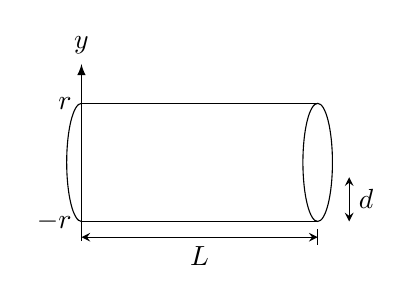
\begin{tikzpicture}
\pgfmathsetmacro{\r}{0.75}
\pgfmathsetmacro{\L}{3}
\draw[-latex](0,-\r-0.25)--(0,\r+0.5)node[above]{$y$};
\draw([shift={(90:1/4*\r cm and \r cm)}]0,0) arc (90:270:1/4*\r cm and \r cm);
\draw(\L,0) circle (1/4*\r cm and \r cm);
\draw(0,-\r)node[left]{$-r$}--++(\L,0);
\draw(0,\r)node[left]{$r$}--++(\L,0);
\draw[stealth-stealth](0,-\r-0.2)--++(\L,0)node[pos=0.5,below]{$L$};
\draw(\L,-\r-0.1)--++(0,-0.2);
\draw[stealth-stealth](\L+0.4,-\r)--++(0,3/4*\r)node[pos=0.5,right]{$d$};
\end{tikzpicture}
\caption{تیل کا حوض (سوال \حوالہ{سوال_طریقہ_حوض_تیل})}
\label{شکل_سوال_طریقہ_حوض_تیل}
\end{figure}

\ابتدا{سوال}
کسی بھی \عددی{a} اور \عددی{b} کے لئے \عددی{\int_a^b\sqrt{x-x^2}\dif x} کی زیادہ سے زیادہ قیمت کیا ممکن ہے؟ اپنے جواب کی وجہ پیش کریں۔\\
جواب:\quad
$\tfrac{\pi}{8}$
\انتہا{سوال}
%==============
\ابتدا{سوال}
کسی بھی \عددی{a} اور \عددی{b} کے لئے \عددی{\int_a^b x\sqrt{x-x^2}\dif x} کی زیادہ سے زیادہ قیمت کیا ممکن ہے؟ اپنے جواب کی وجہ پیش کریں۔
\انتہا{سوال}
%==============
\موٹا{کمپیوٹر الجبرائی نظام}\\
 کمپیوٹر میں الجبرا کے کئی پروگرام پائے جاتے ہیں۔ان میں سے ایک پروگرام \اصطلاح{میکسما}\فرہنگ{میکسما}\حاشیہب{maxima}\فرہنگ{maxima} کہلاتا ہے جو نہایت طاقتور پروگرام ہے۔ متغیر \عددی{x} کے تفاعل \عددی{f(x)} کا غیر قطعی تکمل حاصل کرنے کے لئے میکسما میں \عددی{integrate(f,x)} لکھنا ہو گا۔اسی طرح \عددی{a} تا \عددی{b} قطعی تکمل کے لئے \عددی{integrate(f,x,a,b)} لکھنا ہو گا۔ میکسما یا الجبرا کے کسی دوسرے پروگرام کو سیکھ کر اس کی مدد  سوال \حوالہ{سوال_طریقہ_کمپیوٹر_تکمل_الف} اور سوال \حوالہ{سوال_طریقہ_کمپیوٹر_تکمل_ب} کو حل کریں۔

\ابتدا{سوال}\شناخت{سوال_طریقہ_کمپیوٹر_تکمل_الف}
\begin{multicols}{3}
\begin{enumerate}[a.]
\item
$\int x\ln x\dif x$
\item
$\int x^2\ln x\dif x$
\item
$\int x^3\ln x\dif x$
\item
آپ کو کیا نقش نظر آتا ہے؟ تکمل \عددی{\int x^4\ln x\dif x} کے کلیہ کی پیش گوئی کریں۔ کمپیوٹر سے اس کی تصدیق کریں۔
\item
تکمل \عددی{\int x^n\ln x\dif x,\, n\ge 1} کا کلیہ کیا ہو گا؟ کمپیوٹر سے اس کی تصدیق کریں۔
\end{enumerate}
\end{multicols}
\انتہا{سوال}
%=====================
\ابتدا{سوال}\شناخت{سوال_طریقہ_کمپیوٹر_تکمل_ب}
\begin{multicols}{3}
\begin{enumerate}[a.]
\item
$\int \frac{\ln x}{x^2}\dif x$
\item
$\int \frac{\ln x}{x^3}\dif x$
\item
$\int \frac{\ln x}{x^4}\dif x$
\item
آپ کو کیا نقش نظر آتا ہے؟ تکمل \عددی{\int \frac{\ln x}{x^5}\dif x} کے کلیہ کی پیش گوئی کریں۔ کمپیوٹر سے اس کی تصدیق کریں۔
\item
تکمل \عددی{\int\tfrac{\ln x}{x^n}\dif x,\, n\ge 2} کا کلیہ کیا ہو گا؟ کمپیوٹر سے اس کی تصدیق کریں۔
\end{enumerate}
\end{multicols}
\انتہا{سوال}
%=====================
\ابتدا{سوال}
(ا) درج ذیل تکمل کو کمپیوٹر کی مدد سے حل کریں، جہاں \عددی{n} اختیاری مستقل ہے۔
\begin{align*}
\int_0^{\pi/2}\frac{\sin^n x}{\sin^n x+\cos^n x}\dif x
\end{align*}
کیا آپ کا کمپیوٹر پروگرام اس کو حل کر پاتا ہے؟   (ب) اختیاری مستقل \عددی{n=1,2,3,5,7} لیتے ہوئے تکمل کی قیمت تلاش کریں۔ نتائج کی پیچیدگی پر تبصرہ کریں۔ (ج) اب \عددی{x=\tfrac{\pi}{2}-u} پر کر کے نئے اور پرانے تکمل کا مجموعہ لیں۔ اب درج ذیل تکمل کی  قیمت کیا ہے؟
\begin{align*}
\int_0^{\pi/2}\frac{\sin^nx}{\sin^nx+\cos^nx}\dif x
\end{align*}
آپ دیکھ سکتے ہیں کہ معمولی سی ریاضیاتی عمل سے تکمل کتنا آسان ہو سکتا ہے۔\\
جواب:\quad
$\tfrac{\pi}{4}$
\انتہا{سوال}
%=====================

\حصہ{غیر مناسب تکمل}\شناخت{حصہ_تکمل_کی_ترکیب_غیر_مناسب_تکمل}
اب تک قطعی تکمل پر ہم دو شرائط لاگو کرتے آ رہے ہیں۔ پہلی شرط میں تکمل کا دائرہ کار \عددی{a} تا \عددی{b} کا متناہی ہونا لازمی تھا۔ دوسری شرط میں متکمل کا سعت متناہی ہونا ضروری تھا۔ حقیقت میں ہمیں عموماً ایسی صورت سے واسطہ پڑتا ہے جہاں ان میں سے ایک شرط یا دونوں شرائط  مطمئن نہ ہوتے ہوں۔ زیر منحنی \عددی{y=\tfrac{\ln x}{x^2}} وقفہ \عددی{x=1} تا \عددی{x=\infty} رقبہ، لامتناہی دائرہ کار کی مثال ہے (شکل \حوالہ{شکل_طریقہ_کیا_رقبہ_متناہی}-الف)۔ اسی طرح زیر منحنی \عددی{y=\tfrac{1}{\sqrt{x}}}  وقفہ \عددی{x=0} تا \عددی{x=1} رقبہ، لامتناہی سعت کی مثال ہے (شکل \حوالہ{شکل_طریقہ_کیا_رقبہ_متناہی}-ب)۔ ہم دونوں مثالوں پر ایک ہی طرح  غور کرتے ہیں۔ ہم پوچھتے  ہیں کہ دائرہ کار ذرہ کم کرنے سے تکمل کتنا ہو گا اور اس کے بعد دائرہ کار کو لامتناہی تک پہنچاتے ہوئے تکمل کا حد تلاش کرتے ہیں۔ اسی طرح ہم متکمل کو متناہی رکھتے ہوئے تکمل دریافت کر کے متکمل کو لامتناہی تک پہنچاتے ہوئے تکمل کا حد تلاش کرتے ہیں۔
\begin{figure}
\centering
\begin{subfigure}{0.45\textwidth}
\centering
\begin{tikzpicture}[font=\small,declare function={f(\x)=ln(\x)/(\x^2);}]
\begin{axis}[small, axis lines=middle,xlabel={$x$},ylabel={$y$},xlabel style={at={(current axis.right of origin)},anchor=west},ylabel style={at={(current axis.above origin)},anchor=south},xtick={1,2,3,4,5,6},ytick={0.1,0.2},xmin=0,enlargelimits=true,axis on top]
\addplot[name path=fun,smooth,domain=1:7]{f(x)}node[pos=0.5,right,yshift=1ex]{$y=\frac{\ln x}{x^2}$};
\path[name path=xaxis](1,0)--(7,0);
\addplot[lgray] fill between[of=xaxis and fun];
\end{axis}
\end{tikzpicture}
\caption{}
\end{subfigure}\hfill
\begin{subfigure}{0.45\textwidth}
\centering
\begin{tikzpicture}[font=\small,declare function={f(\x)=1/sqrt(\x);}]
\begin{axis}[small, axis lines=middle,xlabel={$x$},ylabel={$y$},xlabel style={at={(current axis.right of origin)},anchor=west},ylabel style={at={(current axis.above origin)},anchor=south},xtick={1},ytick={1},enlargelimits=true,axis on top]
\addplot[name path=fun,smooth,domain=0.5:1]{f(x)}node[pos=0.5,right,yshift=1ex]{$y=\frac{1}{\sqrt{x}}$};
\draw(1,0)--(1,{f(1)});
\path[name path=xaxis](0.5,0)--(1,0);
\addplot[lgray] fill between[of=xaxis and fun];
\path[name path=kt](0,{f(0.5)})--(0.5,{f(0.5)});
\path[name path=kb](0,0)--(0.5,0);
\addplot[lgray] fill between[of=kt and kb];
\end{axis}
\end{tikzpicture}
\caption{}
\end{subfigure}
\caption{کیا ان منحنیات کے نیچے رقبے متناہی ہیں؟}
\label{شکل_طریقہ_کیا_رقبہ_متناہی}
\end{figure}
%%%%%%%%%%%%%%%%%%%%%%%
\begin{figure}
\centering
\begin{minipage}{0.45\textwidth}
\centering
\begin{tikzpicture}[font=\small,declare function={f(\x)=ln(\x)/(\x^2);}]
\begin{axis}[small, axis lines=middle,xlabel={$x$},ylabel={$y$},xlabel style={at={(current axis.right of origin)},anchor=west},ylabel style={at={(current axis.above origin)},anchor=south},xtick={1,5},xticklabels={$1$,$b$},ytick={0.1,0.2},xmin=0,enlargelimits=true,axis on top]
\addplot[name path=fun,smooth,domain=1:7]{f(x)}node[pos=0.5,right,yshift=1ex]{$y=\frac{\ln x}{x^2}$};
\addplot[name path=fun,smooth,domain=1:5,draw=none]{f(x)};
\path[name path=xaxis](1,0)--(5,0);
\addplot[lgray] fill between[of=xaxis and fun];
\draw(5,0)--(5,{f(5)});
\end{axis}
\end{tikzpicture}
\caption{زیر منحنی رقبہ (مثال \حوالہ{مثال_طریقہ_حد_رقبہ_الف})}
\label{شکل_مثال_طریقہ_حد_رقبہ_الف}
\end{minipage}\hfill
\begin{minipage}{0.45\textwidth}
\centering
\begin{tikzpicture}[font=\small,declare function={f(\x)=1/sqrt(\x);}]
\begin{axis}[small, axis lines=middle,xlabel={$x$},ylabel={$y$},xlabel style={at={(current axis.right of origin)},anchor=west},ylabel style={at={(current axis.above origin)},anchor=south},xtick={0.6,1},xticklabels={$a$,$1$},ytick={1},enlargelimits=true,axis on top]
\addplot[smooth,domain=0.5:1]{f(x)}node[pos=0.5,right,yshift=1ex]{$y=\frac{1}{\sqrt{x}}$};
\addplot[name path=fun,smooth,domain=0.6:1,draw=none]{f(x)};
\path[name path=xaxis](0.6,0)--(1,0);
\draw(0.6,0)--(0.6,{f(0.6)});
\draw(1,0)--(1,{f(1)});
\addplot[lgray] fill between[of=xaxis and fun];
\end{axis}
\end{tikzpicture}
\caption{زیر منحنی رقبہ (مثال \حوالہ{مثال_طریقہ_حد_رقبہ_ب})}
\label{شکل_مثال_طریقہ_حد_رقبہ_ب}
\end{minipage}
\end{figure}

\ابتدا{مثال}\شناخت{مثال_طریقہ_حد_رقبہ_الف}
کیا \عددی{x=1} تا \عددی{x=\infty} منحنی \عددی{y=\tfrac{\ln x}{x^2}} کے نیچے رقبہ متناہی ہے؟ ایسا ہونے کی صورت میں اس کی قیمت تلاش کریں۔

حل:\quad
ہم \عددی{x=1} تا \عددی{x=b} اس منحنی کے نیچے رقبہ تلاش کر کے \عددی{b\to \infty} کی صورت میں رقبے کی حد تلاش کرتے ہیں۔ اگر حد متناہی ہو، ہم اس کو لامتناہی منحنی کے نیچے رقبہ تصور کرتے ہیں (شکل \حوالہ{شکل_مثال_طریقہ_حد_رقبہ_الف})۔ آئیں \عددی{x=1} تا \عددی{x=b} رقبہ تلاش کریں۔ 
\begin{align*}
\int_1^b\frac{\ln x}{x^2}\dif x&=\left[(\ln x)\big(-\frac{1}{x}\big)\right]_1^b-\int_1^b\big(-\frac{1}{x}\big)\big(\frac{1}{x}\big)\dif x\\
&=-\frac{\ln b}{b}-\big[\frac{1}{x}\big]_1^b\\
&=-\frac{\ln b}{b}-\frac{1}{b}+1
\end{align*}
بالائی حد \عددی{b\to \infty} کرتے ہوئے رقبے کی حد تلاش کرتے ہیں۔
\begin{align*}
\lim_{b\to\infty}\big[-\frac{\ln b}{b}-\frac{1}{b}+1\big]&=-\big[\lim_{b\to \infty}\frac{\ln b}{b}\big]-0+1\\
&=-\big[\lim_{b\to\infty}\frac{1/b}{1}\big]+1=0+1=1&&\text{\RL{قاعدہ لھوپیٹال}}
\end{align*}
یوں تکملی اظہار میں \عددی{x=1} تا \عددی{x=\infty} زیر منحنی رقبہ درج ذیل ہو گا۔
\begin{align*}
\int_1^{\infty}\frac{\ln x}{x^2}\dif x=\lim_{b\to\infty}\int_1^b\frac{\ln x}{x^2}\dif x=1
\end{align*} 
\انتہا{مثال}
%====================
\ابتدا{مثال}\شناخت{مثال_طریقہ_حد_رقبہ_ب}
کیا \عددی{x=0} تا \عددی{x=1} زیر منحنی \عددی{y=\tfrac{1}{\sqrt{x}}} رقبہ متناہی ہے؟ اگر ایسا ہو تب رقبہ کتنا ہو گا؟

حل:\quad
ہم \عددی{x=a} تا \عددی{x=1} رقبہ تلاش کر کے \عددی{a\to 0^+} کی صورت میں رقبے کی حد پر نظر ڈالتے ہیں۔ اگر یہ حد متناہی ہو تب ہم اس کو \عددی{0} تا \عددی{1} زیر منحنی رقبہ مانتے ہیں (شکل \حوالہ{شکل_مثال_طریقہ_حد_رقبہ_ب})۔
\begin{align*}
\int_a^1\frac{1}{\sqrt{x}}\dif x=\left.2\sqrt{x}\right\vert_a^1=2-2\sqrt{a}
\end{align*}
اب \عددی{a\to 0^+} کرتے ہوئے رقبے کا حد تلاش کرتے ہیں۔
\begin{align*}
\lim_{a\to 0^+}(2-2\sqrt{a})=2-0=2
\end{align*}
یوں تکملی اظہار میں \عددی{0} تا \عددی{1} زیر منحنی رقبہ درج ذیل ہو گا۔
\begin{align*}
\int_0^1\frac{1}{\sqrt{x}}\dif x=\lim_{a\to 0^+}\int_a^1\frac{1}{\sqrt{x}}\dif x=2
\end{align*}
\انتہا{مثال}
%====================

\جزوحصہء{غیر مناسب تکمل}
مثال \حوالہ{مثال_طریقہ_حد_رقبہ_الف} اور مثال \حوالہ{مثال_طریقہ_حد_رقبہ_ب} میں تکمل غیر مناسب ہیں۔

\ابتدا{تعریف}
وہ تکمل جن کے حد لامتناہی ہوں اور وہ تکمل جن کے متکمل وقفہ تکمل کے کسی نقطہ پر لامتناہی قیمت رکھتا ہو \اصطلاح{غیر مناسب تکمل} کہلاتے ہیں۔ اگر تکمل کا حد موجود ہو تب اس حد کو درج ذیل طریقہ سے حاصل کیا جاتا ہے۔
\begin{enumerate}[a.]
\item
اگر وقفہ \عددی{[a,\infty)} پر \عددی{f} استمراری ہو تب درج ذیل ہو گا۔
\begin{align}
\int_a^{\infty}f(x)\dif x=\lim_{b\to\infty}\int_a^bf(x)\dif x
\end{align}
\item
اگر وقفہ \عددی{(-\infty,b]} پر \عددی{f} استمراری ہو تب درج ذیل ہو گا۔
\begin{align}
\int_{-\infty}^bf(x)\dif x=\lim_{a\to-\infty}\int_a^bf(x)\dif x
\end{align}
\item
اگر وقفہ \عددی{(a,b]} پر \عددی{f} استمراری ہو تب درج ذیل ہو گا۔
\begin{align}
\int_a^bf(x)\dif x=\lim_{c\to a^+}\int_c^bf(x)\dif x
\end{align}
\item
اگر وقفہ \عددی{[a,b)} پر \عددی{f} استمراری ہو تب درج ذیل ہو گا۔
\begin{align}
\int_a^bf(x)\dif x=\lim_{c\to b^-}\int_a^cf(x)\dif x
\end{align}
\end{enumerate}
اگر تکمل کا حد متناہی ہو تب ہم کہتے ہیں کہ یہ غیر مناسب تکمل \اصطلاح{مرتکز}\فرہنگ{مرتکز}\فرہنگ{convergent} ہے اور تکمل کے حد کو اس غیر مناسب تکمل کی قیمت تصور کرتے ہیں۔ اگر تکمل کا حد غیر موجود ہو تب ہم کہتے ہیں کہ یہ غیر مناسب تکمل \اصطلاح{منفرج}\فرہنگ{منفرج}\فرہنگ{divergent}  ہے۔
\انتہا{تعریف}
%=====================

تعریف کی پہلی شق مثال \حوالہ{مثال_طریقہ_حد_رقبہ_الف} میں نظر آتی ہے:
\begin{align*}
\int_1^{\infty}\frac{\ln x}{x^2}\dif x&=\lim_{b\to\infty}\int_1^b\frac{\ln x}{x^2}\dif x=1&&\text{\RL{بالائی حد لا متناہی ہے}}
\end{align*}
تعریف کی تیسری شق مثال \حوالہ{مثال_طریقہ_حد_رقبہ_ب} میں نظر آتی ہے:
\begin{align*}
\int_0^1\frac{1}{\sqrt{x}}\dif x&=\lim_{a\to 0^+}\int_a^1\frac{1}{\sqrt{x}}\dif x=2&&\text{\RL{تکمل کے زیریں حد پر متکمل لامتناہی ہے}}
\end{align*}
مذکورہ بالا دونوں صورتوں میں تکمل کا حد متناہی ہے۔ اگلی مثال میں تکمل منفرج ہے۔

\ابتدا{مثال}\شناخت{مثال_طریقہ_منفرج_غیر_مناسب_تکمل}\ترچھا{منفرج غیر مناسب تکمل}\\
درج ذیل تکمل کی مرکوزیت پر غور کریں۔
\begin{align*}
\int_0^1\frac{1}{1-x}\dif x
\end{align*}
حل:\quad
وقفہ \عددی{[0,1)} پر متکمل \عددی{f(x)=\tfrac{1}{1-x}} استمراری ہے  لیکن \عددی{a\to 1^-} کرنے سے یہ لامتناہی ہوتا ہے (شکل \حوالہ{شکل_مثال_طریقہ_منفرج_غیر_مناسب_تکمل})۔ ہم تکمل کی قیمت حاصل کرنے کی کوشش کرتے ہیں۔
\begin{align*}
\lim_{b\to1^-}\int_0^b\frac{1}{1-x}\dif x&=\lim_{b\to 1^-}\big[-\ln\abs{1-x}\big]_0^b\\
&=\lim_{b\to 1^-}[-\ln(1-b)+0]=\infty
\end{align*}
تکمل کا حد لامتناہی ہے لہٰذا یہ منفرج تکمل ہے۔
\انتہا{مثال}
%==================
\begin{figure}
\centering
\begin{minipage}{0.45\textwidth}
\centering
\begin{tikzpicture}[font=\small,declare function={f(\x)=1/(1-\x);}]
\begin{axis}[small, axis lines=middle,xlabel={$x$},ylabel={$y$},xlabel style={at={(current axis.right of origin)},anchor=west},ylabel style={at={(current axis.above origin)},anchor=south},xtick={0.5,1},xticklabels={$b$,$1$},ytick={1},xmin=0,enlargelimits=true,axis on top]
\addplot[smooth,domain=0:0.6]{f(x)}node[pos=0.9,left,yshift=1ex]{$y=\frac{1}{1-x}$};
\addplot[name path=fun,smooth,domain=0:0.5,draw=none]{f(x)};
\path[name path=xaxis](0,0)--(0.5,0);
\addplot[lgray] fill between[of=xaxis and fun];
\draw(0.5,0)--(0.5,{f(0.5)});
\addplot[] plot coordinates {(1,0) (1,{f(0.5)})};
\end{axis}
\end{tikzpicture}
\caption{غیر مناسب منفرج تکمل (مثال \حوالہ{مثال_طریقہ_منفرج_غیر_مناسب_تکمل})}
\label{شکل_مثال_طریقہ_منفرج_غیر_مناسب_تکمل}
\end{minipage}\hfill
\begin{minipage}{0.45\textwidth}
\centering
\begin{tikzpicture}[font=\small,declare function={f(\x)=1/((\x-1)^(2/3)); g(\x)=1/((1-\x)^(2/3));}]
\begin{axis}[small, axis lines=middle,xlabel={$x$},ylabel={$y$},xlabel style={at={(current axis.right of origin)},anchor=west},ylabel style={at={(current axis.above origin)},anchor=south},xtick={0.5,1,1.6,3},xticklabels={$b$,$1$,$c$,$3$},ytick={1},enlargelimits=true,axis on top]
\addplot[smooth,domain=0:0.6]{g(x)};
\addplot[smooth,domain=1.4:3]{f(x)}node[pos=0.25,right,yshift=1ex]{$y=\frac{1}{(x-1)^{2/3}}$};
\addplot[name path=funG,smooth,domain=0:0.5,draw=none]{g(x)};
\path[name path=xaxisG](0,0)--(0.5,0);
\draw(0.5,0)--(0.5,{g(0.5)});
\addplot[lgray] fill between[of=xaxisG and funG];
\addplot[name path=funF,smooth,domain=1.6:3,draw=none]{f(x)};
\path[name path=xaxisF](1.6,0)--(3,0);
\draw(1.6,0)--(1.6,{f(1.6)});
\addplot[lgray] fill between[of=xaxisF and funF];
\addplot[] plot coordinates {(1,0) (1,{f(1.4)})};
\draw(3,0)--(3,{f(3)});
\end{axis}
\end{tikzpicture}
\caption{اندرون نقطہ پر لامتناہی متکمل (مثال \حوالہ{مثال_طریقہ_اندرون_نقطہ_پر_لا_متناہی})}
\label{شکل_مثال_طریقہ_اندرون_نقطہ_پر_لا_متناہی}
\end{minipage}
\end{figure}
%==================
مذکورہ بالا تعریف کو وسعت دیتے ہوئے ان تکمل جن کے زیریں اور بالائی حدود دونوں لامتناہی ہوں پر لاگو کیا جاتا ہے۔ ہم ان پر اسی حصے میں بعد میں غور کریں گے۔ وقفہ تکمل کے اندر نقطہ \عددی{d} پر لامتناہی متکمل کی صورت پر بھی یہ تعریف لاگو کی جاتی ہے۔ ہم ایسے تکمل کو دو ٹکڑوں میں تقسیم کرتے  ہوئے \عددی{a} تا \عددی{b} تکمل کو \عددی{a} تا \عددی{d} تکمل اور \عددی{d} تا \عددی{b} تکمل کا مجموعہ لیتے ہیں۔

\ابتدا{تعریف}
اگر وقفہ \عددی{[a,b]} کے اندرون کسی نقطہ \عددی{d} پر متکمل \عددی{f} کی قیمت لامتناہی ہو تب درج ذیل ہو گا۔
\begin{align}
\int_a^bf(x)\dif x=\int_a^df(x)\dif x+\int_d^bf(x)\dif x
\end{align}
اگر \عددی{a} تا \عددی{d} اور \عددی{d} تا \عددی{b} تکمل مرتکز ہوں تب \عددی{a} تا \عددی{b} تکمل \اصطلاح{مرتکز} ہو گا ورنہ \عددی{a} تا \عددی{b} تکمل \اصطلاح{منفرج} ہو گا۔
\انتہا{تعریف}
%=====================

\ابتدا{مثال}\شناخت{مثال_طریقہ_اندرون_نقطہ_پر_لا_متناہی}\ترچھا{اندرونی نقطہ پر لامتناہی}\\
درج ذیل تکمل کی مرکوزیت پر غور کریں۔
\begin{align*}
\int_0^3\frac{\dif x}{(x-1)^{2/3}}
\end{align*}
حل:\quad
متکمل \عددی{f(x)=\tfrac{1}{(x-1)^{2/3}}} نقطہ \عددی{x=1} پر لامتناہی ہے جبکہ وقفہ \عددی{[0,1)} اور \عددی{(1,3]} پر یہ استمراری ہے (شکل \حوالہ{شکل_مثال_طریقہ_اندرون_نقطہ_پر_لا_متناہی})۔ وقفہ \عددی{[0,3]} پر تکمل کی مرکوزیت وقفہ \عددی{0} تا \عددی{1} اور وقفہ \عددی{1} تا \عددی{3} پر تکمل کی مرکوزیت پر منحصر ہے۔ وقفہ \عددی{[0,1]} پر 
\begin{align*}
\int_0^1\frac{\dif x}{(x-1)^{2/3}}&=\lim_{b\to 1^-}\int_0^b\frac{\dif x}{(x-1)^{2/3}}\\
&=\lim_{b\to 1^-}[3(b-1)^{1/3}-3(0-1)^{1/3}]=3
\end{align*}
اور وقفہ \عددی{[1,3]} پر
\begin{align*}
\int_1^3\frac{\dif x}{(x-1)^{2/3}}&=\lim_{c\to 1^+}\int_c^3\frac{\dif x}{(x-1)^{2/3}}\\
&=\lim_{c\to 1^+}[3(3-1)^{1/3}-3(c-1)^{1/3}]=3\sqrt[3]{2}
\end{align*}
ہو گا۔دونوں حد متناہی ہیں لہٰذا وقفہ \عددی{0} تا \عددی{3} تفاعل \عددی{f} کا تکمل مرتکز ہو گا اور اس کی قیمت \عددی{3+3\sqrt[3]{2}} ہو گی۔
\انتہا{مثال}
%=================
\ابتدا{مثال}\شناخت{مثال_طریقہ_ٹھوس_بگل}
محور \عددی{x} کے عمودی ایک بگل کا رقبہ عمودی تراش دائری قرص ہیں جن کے قطر وقفہ \عددی{-\infty<x\le \ln 2} پر محور \عددی{x} سے  منحنی \عددی{y=e^x} تک ہیں (شکل \حوالہ{شکل_مثال_طریقہ_ٹھوس_بگل})۔ اس بگل کا حجم تلاش کریں۔

حل:\quad
ایک علامتی رقبہ عمودی تراش کا رقبہ
\begin{align*}
S(x)=\pi (\text{\RL{رداس}})^2=\pi\big(\frac{1}{2}y\big)^2=\frac{\pi}{4}e^{2x}
\end{align*}
ہو گا۔ہم \عددی{b\to-\infty} کرتے ہوئے \عددی{b} تا \عددی{\ln 2} تک حجم کی حد کو بگل کا حجم مانتے ہیں۔ ہم حصہ \حوالہ{حصہ_استعمال_تکمل_ترکیب_ٹکیاں} کی طرح ٹکیاں کاٹ کر حجم تلاش کرتے ہیں۔
\begin{align*}
H&=\int_b^{\ln 2}S(x)\dif x=\int_b^{\ln 2}\frac{\pi}{4}e^{2x}\dif x=\left.\frac{\pi}{8}e^{2x}\right\vert_b^{\ln 2}\\
&=\frac{\pi}{8}(e^{\ln 4}-e^{2b})=\frac{\pi}{8}(4-e^{2b})
\end{align*}
اب \عددی{b\to-\infty} کرنے سے \عددی{e^{2b}\to 0} لہٰذا \عددی{H\to \tfrac{\pi}{8}(4-0)=\tfrac{\pi}{2}} ہوتا ہے۔یوں  بگل کا حجم \عددی{\tfrac{\pi}{2}} ہو گا۔ 
\انتہا{مثال}
%======================
\begin{figure}
\centering
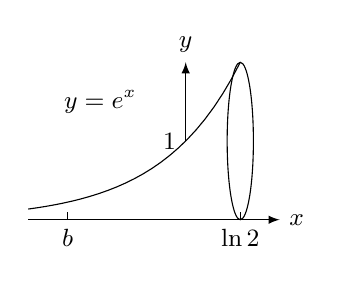
\begin{tikzpicture}[font=\small,declare function={f(\x)=e^(\x);}]
\pgfmathsetmacro{\b}{ln(2)}
\pgfmathsetmacro{\rb}{1/2*f(\b)}
\draw[-latex](-2,0)--(\b+0.5,0)node[right]{$x$};
\draw[-latex](0,{f(0)})node[left]{$1$}--(0,2)node[above]{$y$};
\draw plot [domain=-2:\b]({\x},{f(\x)});
\draw(\b,\rb) circle (1/6*\rb cm and \rb cm);
\draw (-1.5,0)node[below]{$b$}--++(0,0.1)  (\b,0)node[below]{$\ln 2$}--++(0,0.1);
\draw(-0.5,1.5)node[left]{$y=e^x$};
\end{tikzpicture}
\caption{ٹھوس بگل کا حجم (مثال \حوالہ{مثال_طریقہ_ٹھوس_بگل})}
\label{شکل_مثال_طریقہ_ٹھوس_بگل}
\end{figure}

\ابتدا{مثال}
تکمل \عددی{\int_2^{\infty}\tfrac{x+3}{(x-1)(x^2+1)}\dif x} حل کریں۔

حل:
\begin{align*}
\int_2^{\infty}\frac{x+3}{(x-1)(x^2+1)}\dif x&=\lim_{b\to \infty}\int_2^b\frac{x+3}{(x-1)(x^2+1)}\dif x\\
&=\lim_{b\to\infty}\int_2^b\big(\frac{2}{x-1}-\frac{2x+1}{x^2+1}\big)\dif x&&\text{\RL{جزوی کسر}}\\
&=\lim_{b\to\infty}\big[2\ln(x-1)-\ln(x^2+1)-\tan^{-1}x\big]_2^b\\
&=\lim_{b\to\infty}\big[\ln\frac{(x-1)^2}{x^2+1}-\tan^{-1}x\big]_2^b&&\text{\RL{لوگارتھمی اجزاء یکجا}}\\
&=\lim_{b\to \infty}\big[\ln\frac{(b-1)^2}{b^2+1}-\tan^{-1}b\big]-\ln\big(\frac{1}{5}\big)+\tan^{-1}2\\
&=0-\frac{\pi}{2}+\ln 5+\tan^{-1}2\approx 1.1458
\end{align*}
\انتہا{مثال}
%=====================

آپ نے دیکھا کہ \عددی{b\to \infty} کر کے حد کی تلاش سے پہلے ہم نے لوگارتھمی اجزاء کو یکجا کیا۔ اگر ہم ایسا نہ کرتے تب ہمیں درج ذیل نا قابل معلوم مقدار ملتی۔
\begin{align*}
\lim_{b\to \infty} [(2\ln(b-1))-\ln(b^2+1)]=\infty-\infty
\end{align*} 

\جزوحصہء{$-\infty$ سے $\infty$ تک تکمل}
روشنی، بجلی اور  صدا پر غور کرنے سے ایسے تکمل حاصل ہوتے ہیں جن کے دونوں حد لامتناہی ہوتے ہیں۔ اگلا تعریف ان کی مرکوزیت پر ہے۔

\ابتدا{تعریف}
اگر وقفہ \عددی{(-\infty,\infty)} پر \عددی{f} استمراری ہو اور اگر \عددی{\int_{-\infty}^af(x)\dif x} اور \عددی{\int_a^{\infty}f(x)\dif x} دونوں مرتکز ہوں تب ہم کہتے ہیں کہ \عددی{\int_{-\infty}^{\infty}f(x)\dif x} مرتکز ہے اور اس کی قیمت 
\begin{align}\label{مساوات_طریقہ_لامتناہی_حدود_کا_تکمل}
\int_{-\infty}^{\infty}f(x)\dif x=\int_{-\infty}^af(x)\dif x+\int_a^{\infty}f(x)\dif x
\end{align}
مانتے ہیں۔اگر دائیں ہاتھ ایک بھی تکمل منفرج ہو تب \عددی{-\infty} سے \عددی{\infty} تک \عددی{f} کا تکمل منفرج ہو گا۔
\انتہا{تعریف}
%=====================

ہم یہ دکھا سکتے ہیں کہ مساوات \حوالہ{مساوات_طریقہ_لامتناہی_حدود_کا_تکمل} میں \عددی{a} کی قیمت اہمیت نہیں رکھتی ہے۔ ہم \عددی{a} کی کوئی بھی موزوں قیمت لے کر  \عددی{\int_{-\infty}^{\infty}f(x)\dif x} کی مرکوزیت دریافت کر سکتے ہیں۔

تفاعل \عددی{f} کا \عددی{-\infty} سے \عددی{\infty} تک تکمل \عددی{\lim_{b\to\infty}\int_{-b}^bf(x)\dif x} سے مختلف ہو سکتا ہے، جو \عددی{\int_{-\infty}^{\infty}f(x)\dif x} کی عدم مرکوزیت کی صورت میں بھی موجود ہو سکتا ہے (سوال \حوالہ{سوال_طریقہ_عجیب_حقیقت})۔

\ابتدا{مثال}\شناخت{مثال_طریقہ_لامتناہی_خطہ_کا_رقبہ_الف}
\begin{align*}
\int_{-\infty}^{\infty}\frac{\dif x}{1+x^2}&=\int_{-\infty}^0\frac{\dif x}{1+x^2}+\int_0^{\infty}\frac{\dif x}{1+x^2}&&\text{\RL{مساوات \حوالہ{مساوات_طریقہ_لامتناہی_حدود_کا_تکمل} میں $a=0$}}\\
&=\lim_{b\to-\infty}[\tan^{-1}x]_b^0+\lim_{c\to\infty}[\tan^{-1}x]_0^c\\
&=\lim_{b\to-\infty}[\tan^{-1}0-\tan^{-1}b]+\lim_{c\to\infty}[\tan^{-1}c-\tan^{-1}0]\\
&=0-\big(-\frac{\pi}{2}\big)+\frac{\pi}{2}-0=\pi
\end{align*}
ہم محور \عددی{x} اور منحنی \عددی{y=\tfrac{1}{1+x^2}} کے نیچے لامتناہی خطے کے رقبہ کو تکمل کی قیمت مانتے ہیں (شکل \حوالہ{شکل_مثال_طریقہ_لامتناہی_خطہ_کا_رقبہ_الف})۔
\انتہا{مثال}
%====================
\begin{figure}
\centering
\begin{tikzpicture}[font=\small,declare function={f(\x)=1/(1+\x^2);}]
\begin{axis}[small, axis lines=middle,xlabel={$x$},ylabel={$y$},xlabel style={at={(current axis.right of origin)},anchor=west},ylabel style={at={(current axis.above origin)},anchor=south},ytick={1},enlargelimits=true,axis on top]
\addplot[name path=fun,smooth,domain=-3:3]{f(x)}node[pos=0.75,right,yshift=1ex]{$y=\frac{1}{1+x^2}$};
\path[name path=xaxis](-3,0)--(3,0);
\addplot[lgray] fill between[of=xaxis and fun];
\end{axis}
\end{tikzpicture}
\caption{دونوں اطراف لامتناہی منحنی کے نیچے رقبہ متناہی ہے۔}
\label{شکل_مثال_طریقہ_لامتناہی_خطہ_کا_رقبہ_الف}
\end{figure}

\جزوحصہء{تکمل$\int_1^{\infty}\tfrac{\dif x}{x^p}$}
تکمل \عددی{\int_1^{\infty}\tfrac{\dif x}{x^p}} کی مرکوزیت \عددی{p} پر منحصر ہے۔ اگلی مثال میں \عددی{p=1} اور \عددی{p=2} کے لئے اس حقیقت کو دیکھتے ہیں۔

\ابتدا{مثال}\شناخت{مثال_طریقہ_منحنی_کے_نیچے_رقبہ_متناہی_یا_نہیں}
درج ذیل کی مرکوزیت پر غور کریں۔
\begin{align*}
\int_1^{\infty}\frac{\dif x}{x^2} \quad\text{\RL{اور}}\quad  \int_1^{\infty}\frac{\dif x}{x}
\end{align*}
حل:\quad
وقفہ \عددی{[1,\infty)} پر دونوں تفاعل استمراری ہیں اور \عددی{x\to\infty} کرنے سے دونوں کے ترسیم محور \عددی{x} کے قریب آتے ہیں (شکل \حوالہ{شکل_مثال_طریقہ_منحنی_کے_نیچے_رقبہ_متناہی_یا_نہیں}) لہٰذا کیا ہم کہہ سکتے ہیں کہ دونوں منحنیات کے نیچے رقبے متناہی ہوں گے؟ پہلے تکمل کی صورت میں
\begin{align*}
\int_1^{\infty}\frac{\dif x}{x}=\lim_{b\to \infty}\int_1^b\frac{\dif x}{x}=\lim_{b\to \infty}(\ln b-\ln 1)=\infty 
\end{align*}
ہے لہٰذا تکمل منفرج ہو گا۔دوسری تکمل کی صورت میں
\begin{align*}
\int_1^{\infty}\frac{\dif x}{x^2}=\lim_{b\to \infty}\int_1^b \frac{\dif x}{x^2}=\lim_{b\to \infty}\big(-\frac{1}{b}+1\big)=1
\end{align*}
ہے لہٰذا تکمل مرتکز ہے اور اس کی قیمت \عددی{1} ہے۔

عمومی طور \عددی{p>1} کے لئے 
\(\int_1^{\infty}\tfrac{\dif x}{x^p}\)
مرکوز  جبکہ \عددی{p\le 1} کے لئے  منفرج ہو گا (سوال \حوالہ{سوال_تراکیب-تکمل_درکار_مثال_آٹھ})۔
\انتہا{مثال}
%============
\begin{figure}
\centering
\begin{subfigure}{0.45\textwidth}
\centering
\begin{tikzpicture}[font=\small,declare function={f(\x)=1/(\x);}]
\begin{axis}[small, axis lines=middle,xlabel={$x$},ylabel={$y$},xlabel style={at={(current axis.right of origin)},anchor=west},ylabel style={at={(current axis.above origin)},anchor=south},xtick={1,3},xticklabels={$1$,$b$},ytick={1},enlargelimits=true,axis on top]
\addplot[smooth,domain=0.5:3.5]{f(x)}node[pos=0.25,right,yshift=2ex]{$y=\frac{1}{x}$};
\addplot[name path=fun,smooth,domain=1:3,draw=none]{f(x)};
\path[name path=xaxis](1,0)--(3,0);
\addplot[lgray] fill between[of=xaxis and fun];
\draw(1,0)--(1,{f(1)})  (3,0)--(3,{f(3)});
\end{axis}
\end{tikzpicture}
\caption{}
\end{subfigure}\hfill
\begin{subfigure}{0.45\textwidth}
\centering
\begin{tikzpicture}[font=\small,declare function={f(\x)=1/(\x^2);}]
\begin{axis}[small, axis lines=middle,xlabel={$x$},ylabel={$y$},xlabel style={at={(current axis.right of origin)},anchor=west},ylabel style={at={(current axis.above origin)},anchor=south},xtick={1,3},xticklabels={$1$,$b$},ytick={1},enlargelimits=true,axis on top]
\addplot[smooth,domain=0.5:3.5]{f(x)}node[pos=0.25,right,yshift=2ex]{$y=\frac{1}{x^2}$};
\addplot[name path=fun,smooth,domain=1:3,draw=none]{f(x)};
\path[name path=xaxis](1,0)--(3,0);
\addplot[lgray] fill between[of=xaxis and fun];
\draw(1,0)--(1,{f(1)})  (3,0)--(3,{f(3)});
\end{axis}
\end{tikzpicture}
\caption{}
\end{subfigure}
\caption{ایک منحنی کے نیچے رقبہ لا متناہی اور دوسرے کے نیچے متناہی ہے (مثال\حوالہ{مثال_طریقہ_منحنی_کے_نیچے_رقبہ_متناہی_یا_نہیں})۔}
\label{شکل_مثال_طریقہ_منحنی_کے_نیچے_رقبہ_متناہی_یا_نہیں}
\end{figure}

 عموماً \عددی{p>1} کی صورت میں \عددی{\int_1^{\infty}\tfrac{\dif x}{x^p}} مرتکز اور \عددی{p\le 1} کی صورت میں منفرج ہو گا۔

\جزوحصہء{ارتکاز اور انفراج کے پرکھ}
جب کسی غیر مناسب تکمل کی قیمت بلا واسطہ قابل حل نہ ہو (جیسا عموماً ہو گا) تب ہم دو اقدام طریقہ استعمال کرتے ہوئے پہلے ارتکاز ثابت کرتے ہیں اور اس کے بعد اعدادی تراکیب سے تکمل کی قیمت دریافت کرتے ہیں۔ ارتکاز کے بنیادی پرکھ دو ہیں: بلا واسطہ تقابلی پرکھ اور تقابل حد پرکھ ہیں۔

\ابتدا{مثال}\شناخت{مثال_طریقہ_ارتکاز_پرکھ}
تکمل \عددی{\int_1^{\infty}e^{-x^2}\dif x} کے ارتکاز پر غور کریں۔

حل:\quad
تعریف کی رو سے
\begin{align*}
\int_1^{\infty}e^{-x^2}\dif x=\lim_{b\to \infty}\int_1^b e^{-x^2}\dif x
\end{align*}
ہو گا۔ چونکہ یہ تکمل غیر بنیادی ہے لہٰذا اس کو ہم بلا واسطہ حل نہیں کر سکتے ہیں۔ البتہ ہم دکھا سکتے ہیں کہ \عددی{b\to \infty} کرتے ہوئے اس کا حد متناہی ہے۔ہم جانتے ہیں کہ \عددی{\int_1^be^{-x^2}\dif x} متغیر \عددی{b} کا بڑھتا تفاعل ہے لہٰذا \عددی{b\to \infty} کرنے سے یا یہ لامتناہی ہو گا اور یا \عددی{b\to \infty} کرنے سے اس کا حد متناہی ہو گا۔ اب ہر \عددی{ x\ge1} کے لئے \عددی{e^{-x^2}\le e^{-x}} ہے (شکل \حوالہ{شکل_مثال_طریقہ_ارتکاز_پرکھ}) لہٰذا
\begin{align*}
\int_1^be^{-x^2}\dif x\le \int_1^be^{-x}\dif x=e^{-b}+e^{-1}<e^{-1}\approx 0.36788
\end{align*}
ہو گا اور یوں تکمل لامتناہی نہیں ہے۔یوں
\begin{align*}
\int_1^{\infty}e^{-x^2}\dif x=\lim_{b\to\infty}\int_1^be^{-x^2}\dif x
\end{align*}
کسی مخصوص قیمت کو مرتکز ہو گا۔ ہم اس تکمل کی قیمت نہیں جانتے ہیں البتہ اتنا ضرور جانتے ہیں کہ تکمل کی قیمت \عددی{0.37} سے کم ہے۔
\انتہا{مثال}
%======================
\begin{figure}
\centering
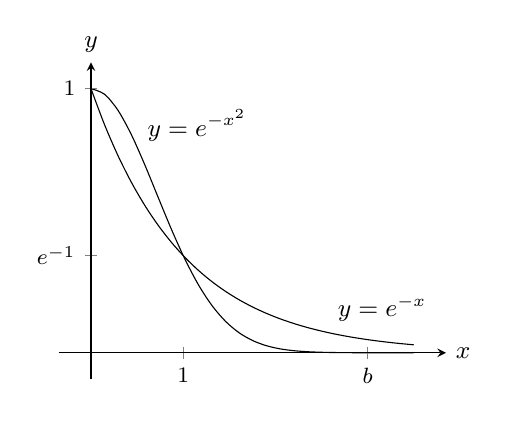
\begin{tikzpicture}[font=\small,declare function={f(\x)=e^(-\x^2);g(\x)=e^(-\x);}]
\pgfmathsetmacro{\k}{e^(-1)}
\begin{axis}[small, axis lines=middle,xlabel={$x$},ylabel={$y$},xlabel style={at={(current axis.right of origin)},anchor=west},ylabel style={at={(current axis.above origin)},anchor=south},xtick={1,3},xticklabels={$1$,$b$},ytick={1,\k},yticklabels={$1$,$e^{-1}$},enlargelimits=true,axis on top]
\addplot[smooth,domain=0:3.5]{f(x)}node[pos=0.15,right,yshift=2ex]{$y=e^{-x^2}$};
\addplot[smooth,domain=0:3.5]{g(x)}node[pos=0.75,right,yshift=2ex]{$y=e^{-x}$};
\end{axis}
\end{tikzpicture}
\caption{وقفہ $x>1$ پر ترسیم $e^{-x^2}$ ترسیم $e^{-x}$ کے نیچے ہے۔}
\label{شکل_مثال_طریقہ_ارتکاز_پرکھ}
\end{figure}

تفاعل \عددی{e^-{x^2}} اور \عددی{e^{-x}} کا پرکھ مثال \حوالہ{مثال_طریقہ_ارتکاز_پرکھ}  میں کیا گیا جو درج ذیل کی ایک مخصوص صورت ہے۔


\ابتدا{مسئلہ}\موٹا{بلا واسطہ تقابلی پرکھ}\فرہنگ{پرکھ!بلا واسطہ تقابلی}\فرہنگ{test!direct comparison}\\
فرض کریں وقفہ \عددی{[a,\infty)} پر \عددی{f} اور \عددی{g} استمراری ہیں اور تمام \عددی{x\ge a} پر \عددی{0\le f(x)\le g(x)} ہے۔ تب درج ذیل ہوں  گے۔
\begin{enumerate}[a.]
\item
اگر \عددی{\int_a^{\infty}g(x)\dif x} مرتکز ہو تب \عددی{\int_a^{\infty}f(x)\dif x} مرتکز ہو گا۔
\item
اگر \عددی{\int_a^{\infty}f(x)\dif x} منفرج ہو تب \عددی{\int_a^{\infty}g(x)\dif x} منفرج ہو گا۔
\end{enumerate}
\انتہا{مسئلہ}
%==================

\ابتدا{مثال}
(ا) چونکہ \عددی{[1,\infty)} پر \عددی{0\le \tfrac{\sin^2x}{x^2}\le \tfrac{1}{x^2}} اور  \عددی{\int_1^{\infty}\tfrac{\dif x}{x^2}} مرتکز ہے لہٰذا  \عددی{\int_1^{\infty}\tfrac{\sin^2x}{x^2}\dif x} مرتکز ہو گا۔\\
(ب) چونکہ \عددی{[1,\infty)} پر \عددی{\tfrac{1}{\sqrt{x^2-0.1}}\ge \tfrac{1}{x}} اور  \عددی{\int_1^{\infty}\tfrac{\dif x}{x}} منفرج  ہے لہٰذا  \عددی{\int_1^{\infty}\tfrac{\dif x}{\sqrt{x^2-0.1}}} منفرج ہو گا۔
\انتہا{مثال}
%======================

\ابتدا{مسئلہ}\شناخت{مسئلہ_تراکیب_تکمل_تقابل_حد_پرکھ}\فرہنگ{پرکھ!تقابل حد}\فرہنگ{test!limit comparison}\موٹا{تقابل حد پرکھ}\\
اگر \عددی{[a,\infty)} پر مثبت تفاعل \عددی{f} اور \عددی{g} استمراری ہوں اور اگر
\begin{align*}
\lim_{x\to\infty}\frac{f(x)}{g(x)}&=L&&(0<L<\infty)
\end{align*}
ہو تب \عددی{\int_a^{\infty}f(x)\dif x} اور \عددی{\int_a^{\infty}g(x)\dif x} دونوں یا مرتکز ہوں گے اور یا دونوں منفرج ہوں گے۔
\انتہا{مسئلہ}
%============================

حصہ \حوالہ{حصہ_ماورائی_اضافی_شرح_نمو} کی زبان میں مسئلہ \حوالہ{مسئلہ_تراکیب_تکمل_تقابل_حد_پرکھ} کہتا ہے کہ اگر \عددی{x\to\infty} پر  دو تفاعل ایک ہی شرح سے بڑھتے ہوں تب \عددی{a} سے \عددی{\infty} تک ان دونوں کے تکمل کا رویہ ایک دوسرے جیسا ہو گا۔ دونوں مرتکز یا دونوں منفرج ہوں گے۔ اس کا ہرگز یہ مطلب نہیں ہے کہ ان دو تکمل کی قیمت ایک دوسرے جیسی ہو گی۔

\ابتدا{مثال}\شناخت{مثال_طریقہ_رویہ_تفاعل}
درج ذیل کا آپس میں تقابل حد پرکھ کی مدد سے موازنہ کریں۔
\begin{align*}
\int_1^{\infty}\frac{\dif x}{x^2},\quad \int_1^{\infty}\frac{\dif x}{1+x^2}
\end{align*}
حل:\quad
ہم \عددی{f(x)=\tfrac{1}{x^2}} اور \عددی{g(x)=\tfrac{1}{1+x^2}} لیتے ہیں۔ یوں
\begin{align*}
\lim_{x\to\infty}\frac{f(x)}{g(x)}&=\lim_{x\to \infty}\frac{1/x^2}{1/(1+x^2)}\\
&=\lim_{x\to\infty}\frac{1+x^2}{x^2}=\lim_{x\to\infty}\big(\frac{1}{x^2}+1\big)=0+1=1
\end{align*}
متناہی مثبت حد ہے (شکل \حوالہ{شکل_مثال_طریقہ_رویہ_تفاعل})۔ اب چونکہ \عددی{\int_1^{\infty}\tfrac{\dif x}{x^2}} مرتکز ہے لہٰذا \عددی{\int_1^{\infty}\tfrac{\dif x}{1+x^2}} بھی مرتکز ہو گا۔

دونوں تکمل کی قیمتیں البتہ مختلف ہیں۔
\begin{align*}
\int_1^{\infty}\frac{\dif x}{x^2}&=1&&\text{\RL{مثال \حوالہ{مثال_طریقہ_منحنی_کے_نیچے_رقبہ_متناہی_یا_نہیں}}}\\
\int_1^{\infty}\frac{\dif x}{1+x^2}&=\lim_{b\to \infty}\int_1^b\frac{\dif x}{1+x^2}\\
&=\lim_{b\to\infty}[\tan^{-1}b-\tan^{-1}1]=\frac{\pi}{2}-\frac{\pi}{4}=\frac{\pi}{4}
\end{align*}

\انتہا{مثال}
%=================
\begin{figure}
\centering
\begin{tikzpicture}[font=\small,declare function={f(\x)=1/(\x^2); g(\x)=1/(1+\x^2);}]
\begin{axis}[small, axis lines=middle,xlabel={$x$},ylabel={$y$},xlabel style={at={(current axis.right of origin)},anchor=west},ylabel style={at={(current axis.above origin)},anchor=south},xtick={1,2,3},ytick={1},enlargelimits=true,axis on top]
\addplot[smooth,domain=0.9:3]{f(x)}node[pos=0.25,right,yshift=1ex]{$y=\frac{1}{x^2}$};
\addplot[smooth,domain=0:3]{g(x)}node[pos=0.5,below left,yshift=-1ex]{$y=\frac{1}{1+x^2}$};
\end{axis}
\end{tikzpicture}
\caption{تفاعل برائے مثال \حوالہ{مثال_طریقہ_رویہ_تفاعل}}
\label{شکل_مثال_طریقہ_رویہ_تفاعل}
\end{figure}

\ابتدا{مثال}
چونکہ \عددی{\int_1^{\infty}\tfrac{\dif x}{e^x}} مرتکز ہے اور
\begin{align*}
\lim_{x\to\infty}\frac{1/e^x}{3/(e^x+5)}&=\lim_{x\to\infty}\frac{e^x+5}{3e^x}\\
&=\lim_{x\to\infty}\big(\frac{1}{3}+\frac{5}{3e^x}\big)=\frac{1}{3}+0=\frac{1}{3}
\end{align*}
مثبت متناہی حد ہے لہٰذا \عددی{\int_1^{\infty}\tfrac{3}{e^x+5}\dif x} مرتکز ہو گا۔  جہاں تک غیر متناسب تکمل کی ارتکاز کی بات ہے \عددی{\tfrac{3}{e^x+5}} اور \عددی{\tfrac{1}{e^x}} کا رویہ ایک دوسرے جیسا ہے۔ 
\انتہا{مثال}
%=========================

\حصہء{سوالات}
\موٹا{غیر مناسب تکمل}\\
سوال \حوالہ{سوال_طریقہ_غیر_مناسب_بغیر_جدول_الف} تا سوال \حوالہ{سوال_طریقہ_غیر_مناسب_بغیر_جدول_ب} کو جدول کلیات تکمل کی مدد کے بغیر حل کریں۔

\ابتدا{سوال}\شناخت{سوال_طریقہ_غیر_مناسب_بغیر_جدول_الف}
$\int_0^{\infty}\frac{\dif x}{x^2+1}$\\
جواب:\quad
$\tfrac{\pi}{2}$
\انتہا{سوال}
%==========================
\ابتدا{سوال}
$\int_1^{\infty}\frac{\dif x}{x^{1.001}}$
\انتہا{سوال}
%==========================
\ابتدا{سوال}
$\int_0^1\frac{\dif x}{\sqrt{x}}$\\
جواب:\quad
$2$
\انتہا{سوال}
%==========================
\ابتدا{سوال}
$\int_0^4\frac{\dif x}{\sqrt{4-x}}$
\انتہا{سوال}
%==========================
\ابتدا{سوال}
$\int_{-1}^1\frac{\dif x}{x^{2/3}}$\\
جواب:\quad
$6$
\انتہا{سوال}
%==========================
\ابتدا{سوال}
$\int_{-8}^1\frac{\dif x}{x^{1/3}}$
\انتہا{سوال}
%==========================
\ابتدا{سوال}
$\int_0^1\frac{\dif x}{\sqrt{1-x^2}}$\\
جواب:\quad
$\tfrac{\pi}{2}$
\انتہا{سوال}
%==========================
\ابتدا{سوال}
$\int_0^1\frac{\dif r}{r^{0.999}}$
\انتہا{سوال}
%==========================
\ابتدا{سوال}
$\int_{-\infty}^{-2}\frac{2\dif x}{x^2-1}$\\
جواب:\quad
$\ln 3$
\انتہا{سوال}
%==========================
\ابتدا{سوال}
$\int_{-\infty}^2\frac{2\dif x}{x^2+4}$
\انتہا{سوال}
%==========================
\ابتدا{سوال}
$\int_2^{\infty}\frac{2\dif v}{v^2-v}$\\
جواب:\quad
$\ln 4$
\انتہا{سوال}
%==========================
\ابتدا{سوال}
$\int_2^{\infty}\frac{2\dif t}{t^2-1}$
\انتہا{سوال}
%==========================
\ابتدا{سوال}
$\int_{-\infty}^{\infty}\frac{2x\dif x}{(x^2+1)^2}$\\
جواب:\quad
$0$
\انتہا{سوال}
%==========================
\ابتدا{سوال}
$\int_{-\infty}^{\infty}\frac{x\dif x}{(x^2+4)^{3/2}}$
\انتہا{سوال}
%==========================
\ابتدا{سوال}
$\int_0^1\frac{\theta+1}{\sqrt{\theta^2+2\theta}}\dif\theta$\\
جواب:\quad
$\sqrt{3}$
\انتہا{سوال}
%==========================
\ابتدا{سوال}
$\int_0^2\frac{s+1}{\sqrt{4-s^2}}\dif s$
\انتہا{سوال}
%==========================
\ابتدا{سوال}
$\int_0^{\infty}\frac{\dif x}{(1+x)\sqrt{x}}$\\
جواب:\quad
$\pi$
\انتہا{سوال}
%==========================
\ابتدا{سوال}
$\int_1^{\infty}\frac{\dif x}{x\sqrt{x^2-1}}$
\انتہا{سوال}
%==========================
\ابتدا{سوال}
$\int_0^{\infty}\frac{\dif v}{(1+v^2)(1+\tan^{-1}v)}$\\
جواب:\quad
$\ln(1+\pi/2)$
\انتہا{سوال}
%==========================
\ابتدا{سوال}
$\int_0^{\infty}\frac{16\tan^{-1}x}{1+x^2}\dif x$
\انتہا{سوال}
%==========================
\ابتدا{سوال}
$\int_{-\infty}^0\theta e^{\theta}\dif\theta$\\
جواب:\quad
$-1$
\انتہا{سوال}
%==========================
\ابتدا{سوال}
$\int_0^{\infty}2e^{-\theta}\sin\theta\dif\theta$
\انتہا{سوال}
%==========================
\ابتدا{سوال}
$\int_{-\infty}^{\infty}e^{-\abs{x}}\dif x$\\
جواب:\quad
$1$
\انتہا{سوال}
%==========================
\ابتدا{سوال}
$\int_{-\infty}^{\infty}2xe^{-x^2}\dif x$
\انتہا{سوال}
%==========================
\ابتدا{سوال}
$\int_0^1 x\ln x\dif x$\\
جواب:\quad
$-\tfrac{1}{4}$
\انتہا{سوال}
%==========================
\ابتدا{سوال}
$\int_0^1 (-\ln x)\dif x$
\انتہا{سوال}
%==========================
\ابتدا{سوال}
$\int_0^2 \frac{\dif s}{\sqrt{4-s^2}}$\\
جواب:\quad
$\tfrac{\pi}{2}$
\انتہا{سوال}
%==========================
\ابتدا{سوال}
$\int_0^1 \frac{4r\dif r}{\sqrt{1-r^4}}$
\انتہا{سوال}
%==========================
\ابتدا{سوال}
$\int_1^2\frac{\dif s}{s\sqrt{s^2-1}}$\\
جواب:\quad
$\tfrac{\pi}{3}$
\انتہا{سوال}
%==========================
\ابتدا{سوال}
$\int_2^4\frac{\dif t}{t\sqrt{t^2-4}}$
\انتہا{سوال}
%==========================
\ابتدا{سوال}
$\int_{-1}^4\frac{\dif x}{\sqrt{\abs{x}}}$\\
جواب:\quad
$6$
\انتہا{سوال}
%==========================
\ابتدا{سوال}
$\int_0^2\frac{\dif x}{\sqrt{\abs{x-1}}}$
\انتہا{سوال}
%==========================
\ابتدا{سوال}
$\int_{-1}^{\infty}\frac{\dif \theta}{\theta^2+5\theta+6}$\\
جواب:\quad
$\ln 2$
\انتہا{سوال}
%==========================
\ابتدا{سوال}\شناخت{سوال_طریقہ_غیر_مناسب_بغیر_جدول_ب}
$\int_0^{\infty}\frac{\dif x}{(x+1)(x^2+1)}$
\انتہا{سوال}
%==========================
\موٹا{پرکھ ارتکاز}\\
سوال \حوالہ{سوال_طریقہ_پرکھ_ارتکاز_الف} تا سوال \حوالہ{سوال_طریقہ_پرکھ_ارتکاز_ب} میں تکمل، بلا واسطہ تقابلی پرکھ یا تقابل حد پرکھ کی مدد سے تکمل کو ارتکاز کے لئے پرکھیں۔ اگر ایک سے زیادہ طریقے قابل استعمال ہوں، وہاں اپنی مرضی سے کسی ایک طریقہ کو استعمال کریں۔

\ابتدا{سوال}\شناخت{سوال_طریقہ_پرکھ_ارتکاز_الف}
$\int_0^{\pi/2}\tan\theta\dif\theta$\\
جواب:\quad
منفرج
\انتہا{سوال}
%======================
\ابتدا{سوال}
$\int_0^{\pi/2}\cot\theta\dif \theta$
\انتہا{سوال}
%======================
\ابتدا{سوال}
$\int_0^{\pi}\frac{\sin\theta\dif\theta}{\sqrt{\pi-\theta}}$\\
جواب:\quad
مرتکز
\انتہا{سوال}
%======================
\ابتدا{سوال}
$\int_{-\pi/2}^{\pi/2}\frac{\cos\theta\dif\theta}{(\pi-2\theta)^{1/3}}$
\انتہا{سوال}
%======================
\ابتدا{سوال}
$\int_0^{\ln 2}x^{-2}e^{-1/x}\dif x$\\
جواب:\quad
مرتکز
\انتہا{سوال}
%======================
\ابتدا{سوال}
$\int_0^1\frac{e^{-\sqrt{x}}}{\sqrt{x}}\dif x$
\انتہا{سوال}
%======================
\ابتدا{سوال}
$\int_0^{\pi}\frac{\dif t}{\sqrt{t}+\sin t}$\\
جواب:\quad
مرتکز
\انتہا{سوال}
%======================
\ابتدا{سوال}
$\int_0^1\frac{\dif t}{t-\sin t}$
\quad
اشارہ: \عددی{t\ge 0} کے لئے \عددی{t\ge \sin t} ہو گا۔
\انتہا{سوال}
%======================
\ابتدا{سوال}
$\int_0^2\frac{\dif x}{1-x^2}$\\
جواب:\quad
منفرج
\انتہا{سوال}
%======================
\ابتدا{سوال}
$\int_0^2\frac{\dif x}{1-x}$
\انتہا{سوال}
%======================
\ابتدا{سوال}
$\int_{-1}^1\ln\abs{x}\dif x$\\
جواب:\quad
مرتکز
\انتہا{سوال}
%======================
\ابتدا{سوال}
$\int_{-1}^1-x\ln \abs{x}\dif x$
\انتہا{سوال}
%======================
\ابتدا{سوال}
$\int_1^{\infty}\frac{\dif x}{x^3+1}$\\
جواب:\quad
مرتکز
\انتہا{سوال}
%======================
\ابتدا{سوال}
$\int_4^{\infty}\frac{\dif x}{\sqrt{x}-1}$
\انتہا{سوال}
%======================
\ابتدا{سوال}
$\int_2^{\infty}\frac{\dif v}{\sqrt{v-1}}$\\
جواب:\quad
منفرج
\انتہا{سوال}
%======================
\ابتدا{سوال}
$\int_0^{\infty}\frac{\dif\theta}{1+e^{\theta}}$
\انتہا{سوال}
%======================
\ابتدا{سوال}
$\int_0^{\infty}\frac{\dif x}{\sqrt{x^6+1}}$\\
جواب:\quad
مرتکز
\انتہا{سوال}
%======================
\ابتدا{سوال}
$\int_2^{\infty}\frac{\dif x}{\sqrt{x^2-1}}$
\انتہا{سوال}
%======================
\ابتدا{سوال}
$\int_1^{\infty}\frac{\sqrt{x+1}}{x^2}\dif x$\\
جواب:\quad
مرتکز
\انتہا{سوال}
%======================
\ابتدا{سوال}
$\int_2^{\infty}\frac{x\dif x}{\sqrt{x^4-1}}$
\انتہا{سوال}
%======================
\ابتدا{سوال}
$\int_{\pi}^{\infty}\frac{2+\cos x}{x}\dif x$\\
جواب:\quad
منفرج
\انتہا{سوال}
%======================
\ابتدا{سوال}
$\int_{\pi}^{\infty}\frac{1+\sin x}{x^2}\dif x$
\انتہا{سوال}
%======================
\ابتدا{سوال}
$\int_4^{\infty}\frac{2\dif t}{t^{3/2}-1}$\\
جواب:\quad
مرتکز
\انتہا{سوال}
%======================
\ابتدا{سوال}
$\int_2^{\infty}\frac{\dif x}{\ln x}$
\انتہا{سوال}
%======================
\ابتدا{سوال}
$\int_1^{\infty}\frac{e^x}{x}\dif x$\\
جواب:\quad
منفرج
\انتہا{سوال}
%======================
\ابتدا{سوال}
$\int_{e^e}^{\infty}\ln(\ln x)\dif x$
\انتہا{سوال}
%======================
\ابتدا{سوال}
$\int_1^{\infty}\frac{\dif x}{\sqrt{e^x-x}}$\\
جواب:\quad
مرتکز
\انتہا{سوال}
%======================
\ابتدا{سوال}
$\int_1^{\infty}\frac{\dif x}{e^x-2^x}$
\انتہا{سوال}
%======================
\ابتدا{سوال}
$\int_{-\infty}^{\infty}\frac{\dif x}{\sqrt{x^4+1}}$\\
جواب:\quad
مرتکز
\انتہا{سوال}
%======================
\ابتدا{سوال}\شناخت{سوال_طریقہ_پرکھ_ارتکاز_ب}
$\int_{-\infty}^{\infty}\frac{\dif x}{e^x+e^{-x}}$
\انتہا{سوال}
%======================
\موٹا{نظریہ اور مثالیں}

\ابتدا{سوال}\ترچھا{لامتناہی دائرہ کار کے غیر مناسب تکمل کی قیمت کا اندازہ}\\
(ا) درج ذیل دکھائیں
\begin{align*}
\int_3^{\infty}e^{-3x}\dif x=\frac{1}{3}e^{-9}<\num{0.000042}
\end{align*}
جس کی بنا \عددی{\int_3^{\infty}e^{-x^2}\dif x<0.000042} ہو گا۔ آپ وجہ پیش کریں کہ کیوں \عددی{\int_3^{\infty}e^{-3x}\dif x} کی جگہ \عددی{\int_3^{\infty}e^{-x^2}\dif x} پر کرنے سے پیدا خلل \عددی{\num{0.000042}} سے زیادہ نہیں ہو سکتا ہے۔\\
(ب) تکمل \عددی{\int_0^3e^{-x^2}\dif x} کی قیمت اعدادی تراکیب سے حاصل کریں۔\\
جواب:\quad
(ب) \عددی{\approx \num{0.88621}}
\انتہا{سوال}
%====================
\ابتدا{سوال}\ترچھا{لامتناہی بگل یا رنگ کا لامتناہی ڈبہ}\\
ہم مثال  \حوالہ{مثال_طریقہ_منحنی_کے_نیچے_رقبہ_متناہی_یا_نہیں} میں دیکھ چکے ہیں کہ \عددی{\int_1^{\infty}\tfrac{\dif x}{x}} منفرج ہے۔ یوں منحنی \عددی{y=\tfrac{1}{x},\,\, 1\le x} کو محور \عددی{x} کے گرد گھما کر حاصل سطح طواف کا سطح
\begin{align*}
\int_1^{\infty}2\pi\frac{1}{x}\sqrt{1+\frac{1}{x^4}}\dif x
\end{align*}
منفرج ہو گا۔ ہم دیکھتے ہیں کہ ہر متناہی قیمت \عددی{b>1} کے لئے 
\begin{align*}
\int_1^b2\pi\frac{1}{x}\sqrt{1+\frac{1}{x^4}}\dif x>2\pi\int_1^b\frac{\dif x}{x}
\end{align*}
ہو گا جبکہ ٹھوس جسم کا حجم
\begin{align*}
\int_1^{\infty}\pi\big(\frac{1}{x}\big)^2\dif x
\end{align*}
مرتکز ہے۔ (ا) اس حجم کی قیمت تلاش کریں۔ (ب) بعض اوقات اس جسم طواف کو وہ ڈبہ کہتے ہیں جس میں اتنا رنگ نہیں بھرا جا سکتا ہے جو اسی ڈبے کی اندرون  کو رنگ کر سکے۔ اس پر ایک لمحہ کے لئے غور کریں۔ متناہی مقدار کا رنگ کسی صورت لامتناہی سطح کو رنگ نہیں کر سکتا ہے۔ البتہ اگر ہم اس ڈبے کو رنگ سے بھریں (جو متناہی مقدار ہو گی) تب ڈبے کی اندرونی سطح (جو لامتناہی ہے) کے ہر نقطہ کو رنگ مس کرتا ہے۔ اس ظاہری تضاد کی وجہ پیش کریں۔ 
\انتہا{سوال}
%======================
\ابتدا{سوال}\شناخت{سوال_تراکیب-تکمل_درکار_مثال_آٹھ}
(ا) دکھائیں کہ \عددی{p>1} کے لئے 
\begin{align*}
\int_1^{\infty}\frac{\dif x}{x^p}=\frac{1}{p-1}
\end{align*}
جبکہ \عددی{p<1} کے لئے تکمل لامتناہی ہے۔
ہے۔ مثال  \حوالہ{مثال_طریقہ_منحنی_کے_نیچے_رقبہ_متناہی_یا_نہیں} میں \عددی{p=1} کے لئے تکمل کی قیمت دیکھی گئی۔\\
(ب) دکھائیں کہ \عددی{p<1} کے لئے
\begin{align*}
\int_0^1\frac{\dif x}{x^p}=\frac{1}{1-p}
\end{align*}
جبکہ \عددی{p\ge1} کے لئے تکمل منفرج ہے۔
\انتہا{سوال}
%======================
\ابتدا{سوال}
درج ذیل ہر ایک تکمل کے لئے \عددی{p} کی وہ قیمت تلاش کریں جس کے لئے  تکمل مرتکز ہو۔
\begin{align*}
\int_2^{\infty}\frac{\dif x}{x(\ln x)^p} \quad \text{\RL{(ب)}}\quad\quad \int_1^2\frac{\dif x}{x(\ln x)^p}\quad \text{\RL{(الف)}}
\end{align*}
\انتہا{سوال}
%=================

سوال \حوالہ{سوال_طریقہ_لامتناہی_خطہ_الف} تا سوال \حوالہ{سوال_طریقہ_لامتناہی_خطہ_ب} ربع اول میں منحنی \عددی{y=e^{-x}} اور محور \عددی{x} کے بیچ لامتناہی خطے کے بارے میں ہیں۔

\ابتدا{سوال}\شناخت{سوال_طریقہ_لامتناہی_خطہ_الف}
اس خطے کا رقبہ تلاش کریں۔\\
جواب:\quad
$1$
\انتہا{سوال}
%======================
\ابتدا{سوال}
اس خطے کا وسطانی مرکز تلاش کریں۔
\انتہا{سوال}
%==========================
\ابتدا{سوال}
اس خطے کو محور \عددی{y} کے گرد گھما کر جسم طواف پیدا کیا جاتا ہے۔ اس جسم کا حجم تلاش کریں۔\\
جواب:\quad
$2\pi$
\انتہا{سوال}
%==========================
\ابتدا{سوال}\شناخت{سوال_طریقہ_لامتناہی_خطہ_ب}
اس خطے کو محور \عددی{x} کے گرد گھما کر جسم طواف پیدا کیا جاتا ہے۔ اس جسم کو حجم تلاش کریں۔
\انتہا{سوال}
%==========================
\ابتدا{سوال}
منحنی \عددی{y=\sec x} اور \عددی{y=\tan x} کے بیچ \عددی{x=0} تا \عددی{x=\tfrac{\pi}{2}} خطے کا رقبہ تلاش کریں۔\\
جواب:\quad
$\ln 2$
\انتہا{سوال}
%====================
\ابتدا{سوال}
منحنی \عددی{y=\sec x} اور \عددی{y=\tan x} کے بیچ \عددی{x=0} تا \عددی{x=\tfrac{\pi}{2}} خطے کو محور \عددی{x} کے گرد گھما کر جسم طواف پیدا کیا جاتا ہے۔ (ا) اس جسم کا حجم تلاش کریں۔ (ب) دکھائیں کہ اس جسم کے اندرونی اور بیرونی سطحوں کے رقبے لامتناہی ہیں۔
\انتہا{سوال}
%====================
\ابتدا{سوال}\شناخت{سوال_طریقہ_عجیب_حقیقت}
\عددی{\int_{-\infty}^{\infty}f(x)\dif x} اور \عددی{\lim_{b\to \infty}\int_{-b}^bf(x)\dif x} کی قیمت مختلف ہو سکتی ہے۔ دکھائیں کہ
\begin{align*}
\int_0^{\infty}\frac{2x\dif x}{x^2+1}
\end{align*}
منفرج ہے لہٰذا
\begin{align*}
\int_{-\infty}^{\infty}\frac{2x\dif x}{x^2+1}
\end{align*}
بھی منفرج ہو گا۔ اس کے بعد درج ذیل دکھائیں۔
\begin{align*}
\lim_{b\to \infty}\int_{-b}^b\frac{2x\dif x}{x^2+1}=0
\end{align*}
\انتہا{سوال}
%======================
\ابتدا{سوال}
درج ذیل دلیل پر غور کریں جس کے تحت \عددی{\ln 3=\infty-\infty}  ہو گا۔ اس دلیل میں غلطی تلاش کریں۔ اپنے جواب کی وجہ پیش کریں۔
\begin{align*}
\ln 3&=\ln 1+\ln 3=\ln 1-\ln \frac{1}{3}\\
&=\lim_{b\to \infty}\ln\big(\frac{b-2}{b}\big)-\ln\frac{1}{3}\\
&=\lim_{b\to \infty}\big[\ln \frac{x-2}{x}\big]_3^b\\
&=\lim_{b\to \infty}[\ln(x-2)-\ln x]_3^b\\
&=\lim_{b\to \infty}\int_3^b\big(\frac{1}{x-2}-\frac{1}{x}\big)\dif x\\
&=\int_3^{\infty}\big(\frac{1}{x-2}-\frac{1}{x}\big)\dif x\\
&=\int_3^{\infty}\frac{\dif x}{x-2}-\int_3^{\infty}\frac{\dif x}{x}\\
&=\lim_{b\to \infty}\big[\ln(x-2)\big]_3^b-\lim_{b\to\infty}\big[\ln x\big]_3^b\\
&=\infty-\infty
\end{align*}  
\انتہا{سوال}
%===============
\ابتدا{سوال}
اگر حقیقی اعداد کے ہر وقفہ پر \عددی{f(x)} قابل تکمل ہو اور \عددی{a} اور \عددی{b} حقیقی اعداد ہوں جہاں \عددی{a<b} ہے تب  درج ذیل دکھائیں۔
\begin{enumerate}[a.]
\item
\عددی{\int_{-\infty}^af(x)\dif x} اور \عددی{\int_a^{\infty}f(x)\dif x} صرف اور صرف اس صورت مرتکز ہوں گے جب \عددی{\int_{-\infty}^bf(x)\dif x} اور \عددی{\int_b^{\infty}f(x)\dif x} دونوں مرتکز ہوں۔
\item
اگر مستعمل تکمل مرتکز ہوں تب درج ذیل ہو گا۔
\begin{align*}
\int_{-\infty}^af(x)\dif x+\int_a^{\infty}f(x)\dif x=\int_{-\infty}^bf(x)\dif x+\int_b^{\infty}f(x)\dif x
\end{align*}
\end{enumerate}
\انتہا{سوال}
%====================
\ابتدا{سوال}\شناخت{سوال_طریقہ_جفت_طاق}
(ا) دکھائیں کہ اگر \عددی{f} جفت ہو اور تکمل موجود ہوں تب درج ذیل ہو گا۔
\begin{align*}
\int_{-\infty}^{\infty}f(x)\dif x=2\int_0^{\infty}f(x)\dif x
\end{align*}
(ب) دکھائیں کہ اگر \عددی{f} طاق ہو اور تکمل موجود ہو تب درج ذیل ہو گا۔
\begin{align*}
\int_{-\infty}^{\infty}f(x)\dif x=0
\end{align*}
\انتہا{سوال}
%=========================

سوال\حوالہ{سوال_طریقہ_مرتکز_منفرج_تلاش_الف} تا سوال \حوالہ{سوال_طریقہ_مرتکز_منفرج_تلاش_ب} میں بلا واسطہ حل، تقابلی پرکھ اور سوال \حوالہ{سوال_طریقہ_جفت_طاق} کے نتائج بروئے کار لاتے ہوئے  تکمل کی مرکوزیت یا انفراج معلوم کریں۔ اگر ایک سے زائد طریقہ قابل استعمال ہوں تب اپنی پسند کا طریقہ استعمال کریں۔

\ابتدا{سوال}\شناخت{سوال_طریقہ_مرتکز_منفرج_تلاش_الف}
$\int_{-\infty}^{\infty}\frac{\dif x}{\sqrt{x^2+1}}$\\
جواب:\quad
منفرج
\انتہا{سوال}
%=======================
\ابتدا{سوال}
$\int_{-\infty}^{\infty}\frac{\dif x}{\sqrt{x^6+1}}$
\انتہا{سوال}
%=======================
\ابتدا{سوال}
$\int_{-\infty}^{\infty}\frac{\dif x}{e^x+e^{-x}}$\\
جواب:\quad
مرتکز
\انتہا{سوال}
%=======================
\ابتدا{سوال}
$\int_{-\infty}^{\infty}\frac{e^{-x}\dif x}{x^2+1}$
\انتہا{سوال}
%=======================
\ابتدا{سوال}
$\int_{-\infty}^{\infty}e^{-\abs{x}}\dif x$\\
جواب:\quad
مرتکز
\انتہا{سوال}
%=======================
\ابتدا{سوال}
$\int_{-\infty}^{\infty}\frac{\dif x}{(x+1)^2}$
\انتہا{سوال}
%=======================
\ابتدا{سوال}
$\int_{-\infty}^{\infty}\frac{\abs{\sin x}+\abs{\cos x}}{\abs{x}+1}\dif x$\quad
اشارہ: 
$\abs{\sin \theta}+\abs{\cos\theta}\ge \sin^2\theta+\cos^2\theta$\\
جواب:\quad
منفرج
\انتہا{سوال}
%=======================
\ابتدا{سوال}\شناخت{سوال_طریقہ_مرتکز_منفرج_تلاش_ب}
$\int_{-\infty}^{\infty}\frac{x\dif x}{(x^2+1)(x^2+2)}$
\انتہا{سوال}
%=======================
\موٹا{کمپیوٹر اور استعمال}\\
سوال \حوالہ{سوال_طریقہ_مختلف_اختیاری_مستقل_الف} تا سوال \حوالہ{سوال_طریقہ_مختلف_اختیاری_مستقل_ب} میں کمپیوٹر استعمال کر کے \عددی{p} کی مختلف قیمتوں (بشمول غیر عدد صحیح) کے لئے تکمل پر غور کریں۔ \عددی{p} کی کن قیمتوں کے لئے تکمل مرتکز ہے؟ جب تکمل مرتکز ہو تب اس کی قیمت کتنی ہے؟ \عددی{p} کی مختلف قیمتوں کے لئے تکمل کو ترسیم کریں۔

\ابتدا{سوال}\شناخت{سوال_طریقہ_مختلف_اختیاری_مستقل_الف}
$\int_0^e x^p\ln x\dif x$
\انتہا{سوال}
%======================
\ابتدا{سوال}
$\int_e^{\infty}x^p\ln x\dif x$
\انتہا{سوال}
%============================
\ابتدا{سوال}
$\int_0^{\infty}x^p\ln x\dif x$
\انتہا{سوال}
%============================
\ابتدا{سوال}\شناخت{سوال_طریقہ_مختلف_اختیاری_مستقل_ب}
$\int_{-\infty}^{\infty}x^p\ln\abs{x}\dif x$
\انتہا{سوال}
%============================
\ابتدا{سوال}
درج ذیل  جسے \اصطلاح{سائن تکمل تفاعل}\فرہنگ{تفاعل!سائن تکمل}\حاشیہب{sine integral function}\فرہنگ{function!sine integral} کہتے ہیں بصریات میں اہم کردار ادا کرتا ہے۔
\begin{align*}
\kSi(x)=\int_0^x\frac{\sin t}{t}\dif t
\end{align*}
%
\begin{enumerate}[a.]
\item
متکمل \عددی{\tfrac{\sin t}{t}} کو \عددی{t>0} کے لئے ترسیم کریں۔ \عددی{\kSi} ہر نقطہ پر بڑھتا کہ گھٹتا تفاعل ہے؟ کیا \عددی{x>0} کے لئے آپ کے خیال میں \عددی{\kSi(x)=0} ہو سکتا ہے؟ وقفہ \عددی{0\le x\le 25} پر \عددی{\kSi(x)} ترسیم کر کے اپنے جواب کی تصدیق کریں۔
\item
درج ذیل کی مرکوزیت پر غور کریں۔
\begin{align*}
\int_0^{\infty}\frac{\sin t}{t}\dif t
\end{align*}
ارتکاز کی صورت میں اس کی قیمت تلاش کریں۔
\end{enumerate}
جواب:\quad
(ب) \عددی{\tfrac{\pi}{2}}
\انتہا{سوال}
%====================
\ابتدا{سوال}\شناخت{سوال_تراکیب_تکمل_تفاعل_خلل_اندازاً_قیمت_درکار}
درج ذیل کو \اصطلاح{تفاعل خلل}\فرہنگ{تفاعل!خلل}\حاشیہب{error function}\فرہنگ{function!error} کہتے ہیں۔
\begin{align*}
\erf(x)=\int_0^x\frac{2e^{-t^2}}{\sqrt{\pi}}\dif t
\end{align*}
نظریہ احتمال اور شماریات میں یہ اہم کردار ادا کرتا ہے۔
\begin{enumerate}[a.]
\item
وقفہ \عددی{0\le x\le 25} کے لئے تفاعل خلل کو ترسیم کریں۔
\item
درج ذیل کی مرکوزیت پر غور کریں۔
\begin{align*}
\int_0^{\infty}\frac{2e^{-t^2}}{\sqrt{\pi}}\dif t
\end{align*}
مرکوزیت کی صورت میں اس کی قیمت کیا نظر آتی ہے؟ آپ اپنی (اندازاً) قیمت کی  تصدیق حصہ \عددی{حصہ_بالکثرت_دوہرا_تکملات_قطبی_روپ} کے سوال \حوالہ{سوال_بالکثرت_تفاعل_خلل_قیمت_درکار} میں کر پائیں گے۔
\end{enumerate}
\انتہا{سوال}
%====================
\موٹا{گیما تفاعل اور کلیہ سٹرلنگ}\\
یولر کا \اصطلاح{گیما تفاعل}\فرہنگ{گیما تفاعل}\حاشیہب{Gamma function}\فرہنگ{Gamma function} \عددی{\Gamma(x)} (جس کو \عددی{x} کا گیما کہتے ہیں) تکمل استعمال کرتے ہوئے عدد ضربیہ تفاعل\حاشیہب{factorial function} کو منفی اعداد اور غیر عدد صحیح اعداد تک وسعت دیتا ہے۔ گیما تفاعل کا کلیہ درج ذیل ہے۔
\begin{align*}
\Gamma(x)=\int_0^{\infty}t^{x-1}e^{-1}\dif t,\quad x>0
\end{align*}
ہر مثبت عدد صحیح \عددی{x} کے لئے \عددی{t^{x-1}e^{-t}} کا \عددی{t} کے لحاظ سے \عددی{0} تا \عددی{\infty} تکمل عدد \عددی{\Gamma(x)}  ہو گا۔ شکل \حوالہ{شکل_تکمل_تراکیب_گیما_تفاعل} میں مبدا کے قریب \عددی{\Gamma} کا ترسیم دکھایا گیا ہے۔ 

\begin{figure}
\centering
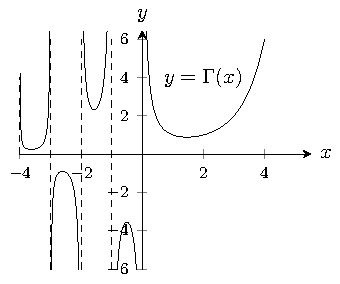
\includegraphics{figOctaveGammaFunction}
\caption{
\عددی{\Gamma(x)} متغیر \عددی{x} کا استمراری تفاعل ہے جس کی قیمت ہر مثبت عدد صحیح \عددی{n+1} پر \عددی{n!} ہے۔ \عددی{\Gamma} کا تعریفی تکمل صرف \عددی{x>0} کے لئے درست ہے لیکن ہم \عددی{\Gamma(x)=\tfrac{\Gamma(x+1)}{x}} (سوال \حوالہ{سوال_تکمل_تراکیب_گیما_وسعت} دیکھیں) کی استعمال سے منفی \عددی{ x} کے لئے \عددی{\Gamma} کو وسعت دے سکتے ہیں۔ 
}
\label{شکل_تکمل_تراکیب_گیما_تفاعل}
\end{figure}


\ابتدا{سوال}\شناخت{سوال_تکمل_تراکیب_گیما_وسعت}\ترچھا{غیر منفی عدد صحیح کے لئے \عددی{\Gamma(n+1)=n!} ہو گا}\\
\begin{enumerate}[a.]
\item
دکھائیں \عددی{\Gamma(1)=1}
\item
اس کے بعد تکمل بالحصص استعمال کرتے ہوئے \عددی{\Gamma(x+1)=x\Gamma(x)} ثابت کریں۔ یوں درج ذیل حاصل ہوں گے۔
\begin{align*}
\Gamma(2)&=1\Gamma(1)=1\\
\Gamma(3)&=2\Gamma(2)=2\\
\Gamma(3)&=3\Gamma(3)=6\\
\vdots&\\
\Gamma(n+1)&=n\Gamma(n)=n!
\end{align*}
\item
الکراجی ماخوذ استعمال کرتے ہوئے ہر غیر منفی عدد صحیح \عددی{n} کے لئے \عددی{\Gamma(n+1)=n\Gamma(n)=n!} کی تصدیق کریں۔
\end{enumerate}
\انتہا{سوال}
%========================
\ابتدا{سوال}\ترچھا{کلیہ سٹرلنگ}\\
اسکاچی ریاضی دان جیمس سٹرلنگ [1692-1770] نے  درج ذیل کلیہ اخذ کیا
\begin{align*}
\lim_{x\to\infty}(\tfrac{e}{x})^x\sqrt{\tfrac{x}{2\pi}}\Gamma(x)=1
\end{align*}
لہٰذا \عددی{x} کی بڑی قیمتوں کے لئے
\begin{gather}
\begin{aligned}\label{مساوات_تکمل_تراکیب_سٹرلنگ_ب}
\Gamma(x)=(\tfrac{x}{e})^x\sqrt{\tfrac{2\pi}{x}}(1+\epsilon(x)),
\end{aligned}\quad\quad
\begin{aligned}
x&\to \infty\\
\epsilon(x)&\to 0
\end{aligned}
\end{gather}

ہو گا۔ اس میں \عددی{\epsilon(x)} رد کرنے سے درج ذیل کلیہ حاصل ہوتا ہے۔
\begin{align}\label{مساوات_تکمل_تراکیب_سٹرلنگ_پ}
\Gamma(x)&\approx (\tfrac{x}{e})^x\sqrt{\tfrac{2\pi}{x}} && \text{\RL{کلیہ سٹرلنگ}}
\end{align}
%
\begin{enumerate}[a.]
\item
مساوات \حوالہ{مساوات_تکمل_تراکیب_سٹرلنگ_پ} اور \عددی{n!=n\Gamma(n)} استعمال کرتے ہوئے  درج ذیل کی تصدیق کریں۔
\begin{align}\label{مساوات_تکمل_تراکیب_سٹرلنگ_ت}
n!&\approx (\tfrac{n}{e})^n\sqrt{2\pi n}&&\text{\RL{تخمین سٹرلنگ}}
\end{align}
جیسا آپ حصہ \حوالہ{حصہ_ترتیب_حد_تلاش_کے_مسائل} کے سوال \حوالہ{سوال_ترتیب_سٹرلنگ} میں دیکھیں گے  مساوات \حوالہ{مساوات_تکمل_تراکیب_سٹرلنگ_ت} سے درج ذیل تخمین حاصل ہوتی ہے۔
\begin{align}\label{مساوات_تکمل_تراکیب_سٹرلنگ_ٹ}
\sqrt[n]{n!}\approx \frac{n}{e}
\end{align}
\item
\عددی{n=10,20,30,\cdots} لیتے ہوئے \عددی{n!} کے لئے  تخمین سٹرلنگ کے نتائج کا کیلکولیٹر سے حاصل نتائج کے ساتھ موازنہ کریں۔
\item
مساوات \حوالہ{مساوات_تکمل_تراکیب_سٹرلنگ_ب} کی بہتر صورت
\begin{align*}
\Gamma(x)=(\tfrac{x}{e})^x\sqrt{\tfrac{2\pi}{x}}e^{1/(12x)}(1+\epsilon(x))
\end{align*}
یا
\begin{align}\label{مساوات_تکمل_تراکیب_سٹرلنگ_ث}
\Gamma(x)=(\tfrac{n}{e})^n\sqrt{2n\pi}e^{1/(12n)}
\end{align}
ہے۔کیلکولیٹر، کلیہ سٹرلنگ اور مساوات \حوالہ{مساوات_تکمل_تراکیب_سٹرلنگ_ث} سے \عددی{10!} کے نتائج کا ایک دوسرے کے ساتھ موازنہ کریں۔ 
\end{enumerate}
\انتہا{سوال}
%==========================
